% main_dark.tex - dark-mode variant of main.tex.
% Shares all chapter inputs with main.tex; differs only in colour scheme.
%
% Build: latexmk -pdf -interaction=nonstopmode main_dark.tex
% Output: main_dark.pdf

\documentclass[a4paper, twoside, 11pt]{report}

%% Language and font encodings
\usepackage[english]{babel}
\usepackage[utf8x]{inputenc}
\usepackage[T1]{fontenc}

%% Sets page size and margins
\usepackage[a4paper,top=3cm,bottom=2cm,left=3cm,right=3cm,marginparwidth=1.75cm]{geometry}

%% Useful packages
\usepackage{amsmath}
\usepackage{graphicx}
\usepackage{float}
\usepackage{array}
\usepackage{ragged2e}
\usepackage[font=small,labelfont=it,textfont=it]{caption}
\usepackage[colorinlistoftodos]{todonotes}
\usepackage{tikz}
\usetikzlibrary{arrows.meta, positioning, shapes.geometric, decorations.pathreplacing, calc}

%% Dark mode colour scheme
\usepackage{xcolor}
\definecolor{darkbg}{HTML}{1B1B1F}      % near-black page background
\definecolor{darkfg}{HTML}{E0E0E0}      % light grey body text
\definecolor{darklink}{HTML}{58A6FF}    % GitHub-dark-style blue for internal links / URLs
\definecolor{darkcite}{HTML}{A5D6A7}    % muted green for citations
\definecolor{darkrule}{HTML}{BDBDBD}    % light-grey table rules (inherited from \color)

\pagecolor{darkbg}
\color{darkfg}

%% hyperref must be loaded last so its colour options resolve correctly
\usepackage[colorlinks=true, linkcolor=darklink, urlcolor=darklink, citecolor=darkcite]{hyperref}
\usepackage{listings}
\lstdefinestyle{transcript}{
  basicstyle=\ttfamily\scriptsize\color{darkfg},
  breaklines=true,
  breakatwhitespace=false,
  columns=fullflexible,
  keepspaces=true,
  showstringspaces=false,
  upquote=true,
  frame=single,
  rulecolor=\color{darkfg},
  framesep=4pt,
  xleftmargin=4pt,
  xrightmargin=4pt,
  aboveskip=6pt,
  belowskip=6pt,
}

\newcolumntype{L}[1]{>{\RaggedRight\arraybackslash}p{#1}}

\title{Beyond Before-and-After: Process-Quality Evaluation of Refactoring Sessions}
\author{Ethan Hosier}
% Update supervisor and other title stuff in title/title.tex

\begin{document}
\input{title/title.tex}

\begin{abstract}
Your abstract goes here
\end{abstract}

\tableofcontents

\chapter{Introduction}
\section{Background}


Refactoring is a routine activity in software development: developers restructure code to improve readability, maintainability, and evolvability while keeping externally observable behaviour the same. Traditional definitions emphasise this preservation of behaviour and describe refactoring as a sequence of small, semantics-preserving transformations \cite{opdyke1992refactoring,fowler1999refactoring,fowler2018refactoring}, and subsequent surveys categorise these refactoring operations and the tools that support them \cite{mens2004survey}. In practice, refactoring is widely encouraged because poorly structured code becomes an obstacle when enhancing and maintaining code, and long-lived systems need continual adjustment (as argued in work building on Lehman’s laws and empirical studies of software maintenance). At the same time, refactoring can be costly: it consumes developer time, introduces risk, and is frequently intertwined with other work such as feature development and bug fixing rather than occurring as isolated “refactoring-only” tasks \cite{murphyhill2009howrefactor,kim2011apilevel}.

\section{Motivation}

Most research and tooling that evaluates refactoring focuses on \textit{outcomes} rather than the \textit{process}. A common approach is to measure refactoring success as a change in static quality indicators between a “before” and “after” state: reductions in code smells, improvements in cohesion/coupling, decreases in complexity, or related metrics to do with maintainability. Typical strands of work include metric-driven detection or prioritisation of candidate refactorings (e.g., using metric changes to separate refactoring-like edits from functional ones, or to choose between different refactoring options), as well as refactoring recommendation systems that rank alternatives by their impact on design metrics. More recent work expands the signals used for guidance by incorporating traceability alongside code metrics when ranking refactoring solutions, and exploring how product/process metrics relate to developers’ motivations to refactor (e.g., studies building on mined refactorings and repository history, and proposals that use LLMs to determine developers' motivations from commit artefacts). Alongside this, there is a substantial line of work that has improved the ability to \textit{detect} refactorings from code changes, notably by using AST-based differencing and structured matching to infer refactoring operations between revisions (e.g., RefactoringMiner and related approaches), which has enabled large-scale empirical studies of how often refactoring happens, what kinds occur, and in what contexts \cite{alikhanifard2025rminer,falleri2024gumtree}.

However, these perspectives evaluate refactoring as a mapping from an initial program state to a final program state, leaving the \textit{trajectory} between those states largely outside the picture. This matters because developers rarely refactor in a single atomic operation: they work through intermediate states, sometimes take detours, redo work, and often accept temporary degradation (e.g., in readability, modular structure, or test/build stability) before arriving at a final outcome. Two developers can arrive at the same end state via very different paths: one might take lots of disruptive steps, bounce between designs, or create avoidable churn, while another might get there via a steadier, more stable sequence. Existing endpoint-only evaluation cannot distinguish these different cases. Meanwhile, research on process realism suggests that refactoring is often ``flossed'' into ongoing development instead of being a separate dedicated task, which increases the chance of mixed-intent steps and noisy traces \cite{murphyhill2009howrefactor}. This makes the quality of the process (how a developer navigates intermediate states) potentially important for both developer productivity and the health of the codebase as it evolves.

Concurrent work has begun to analyse refactoring trajectories under a state/action/observation formalism, qualitatively classifying failure modes of language-model agents on multi-file refactoring tasks \cite{gautam2025refactorbench} and characterising recurring action patterns in software-engineering agent traces \cite{bouzenia2025trajectories}. A recent systematic literature review of LLM-based refactoring research likewise surveys evaluation methodologies and identifies open challenges in this area \cite{alomar2025slr}. As far as we are aware, however, no prior system both (i) scores a developer's refactoring trace against an explicit process-quality metric and (ii) produces counterfactual reference trajectories tied to measurable divergence points. The closest work either synthesises a path to reach an end state (without judging the developer's path) or recommends refactorings on an architectural target (without reference to an observed process). We instantiate the framing in a tool, evaluate it on a 45-session corpus of recorded refactoring sessions with hand-labelled ground truth, and report per-kind precision and recall alongside a sensitivity and ablation analysis of the underlying score formula.

\section{Research Objectives}

We investigate the following thesis question: \textbf{given a known start state and a known end state, can we evaluate the quality of the developer’s refactoring process, and identify points where a better process was available?} The core idea is to explicitly model refactoring as a \textit{process} over states, rather than judging it only by comparing endpoints. To do this, we adopt a state/action/trace framing: snapshots of the codebase are treated as \textit{states}, and developer edits---including IDE refactorings and manual transformations---are treated as \textit{actions} that produce a trace from the start state to the end state.

A core component will be a \textbf{process-quality metric} that scores traces according to criteria that will be defined and justified using existing research on code quality metrics, smell detection validity, and process-level signals. The metric is not assumed to be purely structural: it may incorporate multiple terms capturing endpoint improvement, intermediate-state degradation, churn/disruption, and “safety” proxies such as preserving build and test behaviour, reflecting the known limitations of relying on any one signal alone.

To go beyond scoring a single observed refactoring trace, we construct \emph{counterfactual} alternatives in the form of other \textbf{reference trajectories} between the same start and end states which have been optimised to achieve a higher score under a chosen process-quality metric. This provides a reasonable basis for comparison: analysis can identify \emph{divergence points} where the developer's trajectory deviates from a higher-scoring path, and quantify how much of the gap in resulting refactoring quality is due to each divergence. This extends previous work that synthesises or recommends refactoring sequences: ReSynth synthesises a path to reach a target end state from a developer's partial edits \cite{raychev2013resynth}, Refactoring Navigator suggests refactoring steps to guide a system toward a desired target at an architectural level \cite{lin2016navigator}, and search-based refactoring treats refactoring sequences as an optimisation problem under explicit quality functions \cite{harman2007pareto,mohan2019manyobjective}. While these systems show that refactoring sequences can be generated and optimised, they do not aim to assess the quality of a developer's chosen process under an explicit process-quality objective. In our work, counterfactual generation supports \emph{process evaluation}: it is used to construct a higher-scoring reference trajectory under the chosen metric and to explain key divergence points, rather than to automate the developer's work or to find any arbitrary sequence of steps that can be followed to reach the end state.

\section{Contributions}

Concretely, we make the following contributions:

\begin{itemize}
  \item A process-quality metric for refactoring trajectories, with each term grounded in cited prior work on code quality and developer process signals, and validated by a single-knob sensitivity sweep and a full power-set ablation analysis.
  \item A first-class divergence-point detector that classifies divergence into four kinds (\textsc{ordering}, \textsc{manual\_refactor}, \textsc{rework}, \textsc{hygiene}) and produces a counterfactual reference trajectory for each.
  \item A 45-session hand-recorded corpus on a purpose-built Java fixture, with multi-label ground-truth annotations, together with the experimental drivers (sensitivity, ablation, divergence) used to evaluate the detector against it.
  \item An empirical evaluation of the detector that establishes per-kind precision and recall, surfaces what the score formula measurably captures, and identifies which categories of process improvement the formula is structurally insensitive to.
\end{itemize}

\section{Approach and Scope}

Our approach targets refactoring as it actually occurs in real-world development, including sequences that involve both IDE-supported refactorings and manually performed edits. We initially focus on refactorings in a single language (Java) to allow the use of mature parsing infrastructure, established quality metrics, and state-of-the-art refactoring mining (e.g., RefactoringMiner). A refactoring process is represented as a sequence of steps between code snapshots. Steps may correspond to commits or developer-defined checkpoints, and this representation can be refined using higher granularity IDE data where available.

The final system comprises (i) an IDE plugin for capturing refactoring traces and presenting feedback, and (ii) an analysis component that scores the observed refactoring process and finds higher-scoring alternative trajectories between the same start and end states under a chosen process-quality metric. Rather than attempting all possible refactoring operators in a given state, or calculating globally optimal refactoring trajectories, the goal is to produce a plausible reference trajectory which scores higher on the chosen metric, and to explain the points at which the developer's trajectory diverged from it (e.g., where making a different earlier decision could have avoided churn, reduced temporary quality degradation, or preserved build/test stability).

\begin{figure}[H]
\centering
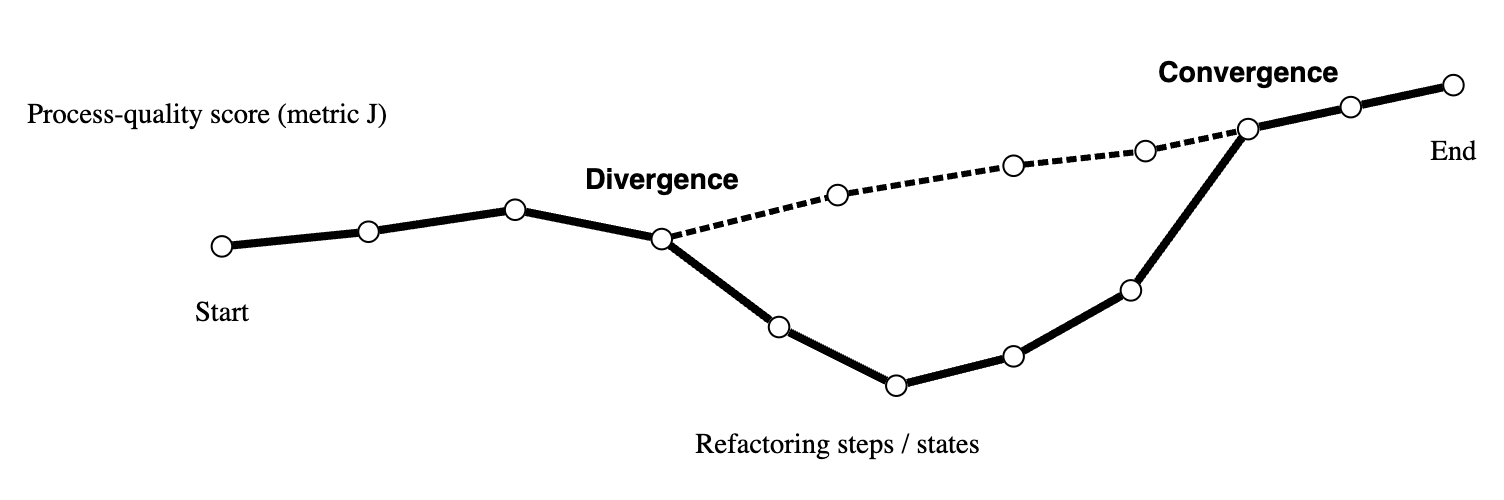
\includegraphics[width=0.8\textwidth]{introduction/divergence_diagram.png}
\caption{Illustration of refactoring trajectories scored by process-quality metric $J$. The solid line shows the developer's observed trajectory, and the dashed line shows a higher-scoring reference trajectory that diverges at an intermediate state and converges near the end.}
\label{fig:divergence}
\end{figure}

\section{Thesis Roadmap}
% TODO: update chapter cross-references to use \ref once the final chapter labels are in place.
The remainder of this thesis is structured as follows. Chapter~2 surveys related work in refactoring evaluation, mining, recommendation and synthesis, and positions our work against that literature. Chapter~3 defines the process-quality metric and the divergence-point detector. Chapter~4 describes the tool's architecture and implementation. Chapter~5 reports experimental results on the 45-session corpus and analyses threats to validity. Chapter~6 concludes and identifies directions for future work.

\chapter{Background}
\label{ch:background}

This chapter reviews the background needed to treat \emph{refactoring as a process}, rather than only as a change between two endpoints. It begins with definitions of refactoring and refactoring sequences (\S\ref{sec:def-framing}), then discusses outcome-based evaluation and the code-quality signals commonly used to judge whether code has improved (\S\ref{sec:outcome-eval}--\S\ref{sec:smells-metrics}). It then reviews refactoring mining, recommendation and sequence synthesis, and IDE-based process tracing (\S\ref{sec:refactoring-mining}--\S\ref{sec:process-aware-logging}). The chapter ends by positioning this project against that work (\S\ref{sec:background-summary}).

\section{Definitions and framing}
\label{sec:def-framing}

\subsection{Refactoring as behaviour-preserving transformation}
Refactoring is usually defined as changing a program's internal structure to improve qualities such as readability or maintainability, while preserving externally observable behaviour. Classic definitions stress that refactoring is built from small, semantics-preserving steps, with safety supported by preconditions and validation such as testing \cite{opdyke1992refactoring,fowler1999refactoring,fowler2018refactoring}. Opdyke's work frames refactorings as program transformations with applicability conditions intended to preserve behaviour under a static approximation \cite{opdyke1992refactoring}. Fowler's catalogue helped popularise refactoring as an incremental developer activity made up of many small operations \cite{fowler1999refactoring,fowler2018refactoring}. Mens and Tourw\'e later survey the wider research landscape, bringing together definitions, taxonomies, and tool support, and emphasising the role of precondition checking and program analysis in automated refactoring \cite{mens2004survey}.

In practice, this clean definition is harder to apply. Developers often refactor while also adding features or fixing bugs, and some refactorings are only partly completed. As a result, it is often ambiguous whether a change seen in version history is a ``pure refactoring''. In this thesis, behaviour preservation is therefore treated as an \emph{intended property} of refactoring steps, while recognising that real traces may include edits with more than one purpose.

\subsection{Atomic refactorings, smells, and sequences}
Research on refactoring often describes refactorings as a set of \emph{operators}, or atomic refactorings, such as \textsc{Extract Method}, \textsc{Move Method}, and \textsc{Rename} \cite{fowler1999refactoring,mens2004survey}. Larger changes can then be understood as sequences of these smaller operations. Code smells are closely related: they are heuristic indicators of possible design problems, and therefore of possible refactoring opportunities \cite{fowler1999refactoring,fowler2018refactoring}. Although smells are not formal correctness criteria, they provide a useful bridge between developer judgement and measurable signals, discussed further in \S\ref{sec:smells-metrics}.

A key distinction in this thesis is between judging only the start and end states of a refactoring, and judging the path taken between them. Two developers may reach the same final code, but one path may involve more temporary degradation, churn, or disruption than the other. These differences can matter for productivity and risk, even when the endpoint looks the same.

\subsection{Representing refactoring as states and actions}
To represent this refactoring path explicitly, we use a state/action/trace model. A codebase snapshot is treated as a \emph{state} $s \in \mathcal{S}$, such as the repository at a particular point in time. An \emph{action} $a \in \mathcal{A}$ is a developer edit step, which may be an IDE-supported refactoring, a manual change, or a mixture of both. A refactoring process is then a \emph{trace}
\[
\tau = (s_0, a_0, s_1, a_1, \dots, a_{T-1}, s_T),
\]
where each action $a_t$ transforms state $s_t$ into $s_{t+1}$. This makes it possible to talk about ``process quality'' as a property of the whole trace $\tau$, rather than only as a comparison between the first and final states $(s_0, s_T)$.

This framing is also close to recent software-engineering work that models agent and developer behaviour as a partially-observable Markov decision process, where a trajectory is a sequence of action and observation pairs \cite{gautam2025refactorbench}. We keep the explicit state notation because this thesis scores the intermediate code states themselves, not only the actions or observations produced along the way.

\section{Outcome-based refactoring evaluation}
\label{sec:outcome-eval}

\subsection{Judging refactoring by the final state}
Refactoring is often evaluated by comparing quality indicators before and after the change. Under this view, a refactoring is successful if the final snapshot improves on the starting snapshot according to selected measures, such as lower coupling, higher cohesion, lower complexity, or fewer code smells. This endpoint-focused view appears both in empirical studies of refactoring impact and in recommendation systems that rank candidate refactorings by their predicted improvement.

A clear example is \emph{search-based refactoring}, where refactoring is treated as an optimisation problem over possible refactoring operations or sequences. Harman and Tratt apply multi-objective search at the design level, treating coupling and cohesion as objectives that may need to be traded off against each other \cite{harman2007pareto}. Later work extends this idea to many-objective settings and adds constraints or preferences for practical concerns such as test coverage or prioritisation \cite{mohan2019manyobjective}. This line of work is useful here because it shows that ``better'' code is not a single fixed property: different quality goals can pull in different directions.

The same endpoint-based idea is also used in refactoring recommendation systems. These systems compare possible refactorings and rank them by the improvement they are expected to produce. Some go beyond code-structure metrics by using information such as requirements traceability, since a design may be easier to maintain when it also supports tasks like impact analysis \cite{wang2018traceability}. More recent work has also looked at how to choose among large sets of candidate refactorings, and which code characteristics are associated with positive or negative effects in practice \cite{nikolaidis2024metricsbased}.

\subsection{What endpoint evaluation captures-and what it misses}
Endpoint-based evaluation is useful when the main concern is whether the final code is better than the starting code under some metric $Q$. It gives recommendation systems a simple strategy: simulate each candidate refactoring and choose the one that gives the largest improvement in $Q$. It is also useful for empirical studies, where refactoring events can be compared with changes in measured code quality. This fits naturally with many existing metrics, since they are defined over a single codebase snapshot.

The weakness of this approach is that it says little about the refactoring process itself. Two developers may reach the same endpoint through very different paths, but endpoint metrics would treat those paths as equivalent. In practice, the intermediate states can still matter: code may become harder to understand for a period of time, the modular structure may be disrupted, or the build and tests may break before being repaired. The path can also be costly in other ways, for example by creating extra churn, making review harder, or increasing integration risk. Empirical work on modularity improvement shows this trade-off clearly: improvements in design metrics can come with substantial structural disruption \cite{paixao2017balancing}. This motivates evaluating not only the final code, but also the stability and cost of the path taken to reach it.

This is the point at which the process view becomes useful. Final-code metrics still matter, but they need to be considered alongside what happened on the way there: whether the work introduced temporary degradation, required rework, created unnecessary churn, or broke build/test stability.

\section{Code smell detection and quality metrics}
\label{sec:smells-metrics}

\subsection{Using code smells as design signals}
Code smells provide a way to connect qualitative design concerns with measurable indicators \cite{fowler1999refactoring}. Smell detectors usually identify these cases either through hand-written rules or learned models. They often rely on structural properties such as size, coupling, and cohesion, with some tools also using lexical or semantic features. One prominent rule-based example is DECOR, which defines smells and design anti-patterns through measurable symptoms and detection rules \cite{moha2010decor}. DECOR is widely used in empirical studies because its definitions are explicit and it can be run efficiently at scale.

Smell detectors are useful, but they should not be treated as ground truth. Comparative studies show that tools can disagree in both precision and recall, and that performance varies across systems and smell types \cite{paiva2017evaluation}. Much of this comes from the practical choices each tool makes, such as thresholds, feature sets, and implementation details. Detectors can also produce false positives, marking code as ``smelly'' even when there is no clear negative impact or when the design reflects an acceptable trade-off \cite{arcellifontana2016falsepositives}. For this reason, smell counts are used in this thesis as one signal among several. They are combined with structural metrics, readability-oriented measures, and process-level safety signals, rather than being allowed to determine the process-quality score on their own.

\subsection{Structural and readability metrics}
Static metrics provide another way to measure code quality at the level of classes, methods, and packages. Common metric families cover coupling, cohesion, complexity, and size, and are often used as indicators of maintainability. These structural measures are useful, but they do not capture everything developers care about when refactoring. Readability is one example: models that combine structural features, such as line structure, with textual features, such as identifier patterns, tend to align better with human judgements of readability \cite{scalabrino2018readability}. This matters for process evaluation because readability and understandability are common reasons for refactoring, and they can change noticeably in intermediate states even if the final code improves.

\subsection{What this means for the process-quality metric}
The process-quality metric $J(\tau)$ uses these signals, but it also has to account for their limitations. The literature suggests three design choices:
\begin{enumerate}
  \item \textbf{Use multiple signals.} No single metric or smell detector gives reliable ground truth across all contexts \cite{paiva2017evaluation,arcellifontana2016falsepositives}. Combining several signals reduces dependence on the quirks of one tool.
  \item \textbf{Separate endpoint improvement from process cost.} Improving the final snapshot is important, but disruption and temporary degradation can still matter even when the endpoint improves \cite{paixao2017balancing}.
  \item \textbf{Keep the components interpretable.} A process critique is more useful when it can point to a specific issue, such as a readability dip, churn spike, or smell increase, rather than only reporting a single opaque score.
\end{enumerate}

A process metric should also include some notion of developer \textbf{effort}, such as the number of steps in the trajectory or the size of the edits between successive states. Fewer steps are not always better, since small steps can reduce risk, but step count and edit size are still useful for identifying unnecessary detours and rework. Similar cost terms are already used alongside structural quality goals in search-based refactoring and recommendation work, for example when trying to improve quality while minimising change \cite{harman2007pareto,mohan2019manyobjective}.

Table~\ref{tab:metric-candidates} summarises the candidate signals, their main benefits and limitations, and examples of Java tooling. The table does not define the final formula for $J(\tau)$, including weights or normalisation. Its purpose is to motivate the signals used later; the precise definition of $J(\tau)$ is given in the methodology chapter and used consistently in the evaluation.

\begin{table}[htbp]
\centering
\small
\begin{tabular}{L{0.19\textwidth} L{0.26\textwidth} L{0.28\textwidth} L{0.19\textwidth}}
\hline
\textbf{Signal} & \textbf{Pros} & \textbf{Cons / threats} & \textbf{Typical tooling} \\
\hline
Structural metrics (coupling/cohesion/\newline complexity/size) &
Widely used; efficient; interpretable at class/method granularity &
Validity depends on context; may incentivise disruptive restructuring; metric interactions &
Static analysis metric extractors; IDE/CI integrations \\
\hline
Smell counts / severity (rule-based) &
Directly targets design issues; aligns with developer's motivations &
Detector disagreement and false positives; threshold sensitivity; context dependence &
DECOR-style detectors \cite{moha2010decor}; other smell tools \cite{paiva2017evaluation} \\
\hline
Readability models &
Closer to human comprehension than structural-only metrics; captures lexical/style clues &
Model generalisation and dataset bias; may be language/style dependent &
Readability predictors \cite{scalabrino2018readability} \\
\hline
Churn / disruption (LOC changed, file moves/renames) &
Captures cost and instability of change; naturally trajectory-oriented &
Churn may be necessary for large refactors; can penalise required restructuring &
VCS mining; diff statistics \\
\hline
Process length / effort (number of steps; edit magnitude) &
Trajectory-native cost signal; discourages detours/rework; easy to compute &
Sensitive to step granularity (commits vs.\ checkpoints vs.\ IDE events); may penalise safe micro-steps; requires calibration &
VCS checkpoints; IDE logs; diff/AST edit size \\
\hline
Build/test preservation signals &
Direct safety signal; aligns with ``behaviour-preserving intent'' &
Requires runnable builds/tests; noisy due to flaky tests; environment dependence &
CI logs; local build/test runs \\
\hline
Traceability-augmented signals &
Reflects maintenance tasks beyond code structure; complements metric-only ranking &
Requires trace links (often unavailable); domain-specific assumptions &
Traceability-based ranking methods \cite{wang2018traceability} \\
\hline
\end{tabular}
\caption{Candidate signals for constructing a process-quality objective. We combine endpoint quality change with trajectory-oriented cost and stability terms, rather than relying on any single indicator.}
\label{tab:metric-candidates}
\end{table}


\section{Refactoring detection and mining from code changes}
\label{sec:refactoring-mining}

\subsection{From diffs to refactoring actions}
To evaluate a process trace in practice, developer actions either need to be captured directly, for example through IDE event logs, or inferred from the differences between snapshots such as bursts of manual user edits. Much of this work uses the second route: given two versions of a program, infer whether a refactoring happened and identify which refactoring types occurred.

\emph{Structured code differencing} is important here because many refactorings are not easy to recognise from line-based diffs alone. AST-based differencing can represent moves, renames, and other non-local edits more directly. GumTree, for example, maps fine-grained AST nodes between program versions and produces edit scripts that better reflect the structural changes developers intended \cite{falleri2024gumtree}. This kind of differencing is often used as the base layer for refactoring detection.

Modern refactoring miners use these structural mappings together with heuristics for particular refactoring types. RefactoringMiner detects a wide range of refactorings between two versions of the code by matching related classes, methods, and fields \cite{alikhanifard2025rminer}. RefDiff takes a similar approach, using similarity heuristics and static analysis to detect common refactoring types in version histories \cite{silva2017refdiff}. For process analysis, tools like these are useful because they can turn a transition $s_t \rightarrow s_{t+1}$ into a set of detected refactoring actions, giving the trace a concrete \emph{action vocabulary}.

\subsection{What refactoring detectors miss}
Refactoring detection tools usually report what kind of refactoring occurred, such as \textsc{Move Method} or \textsc{Extract Class}, and which classes, methods, or fields were involved. This fits the operator-based view of refactoring used in refactoring guides and surveys \cite{fowler1999refactoring,mens2004survey}. However, the literature also reports several limitations that matter for process evaluation.

\paragraph{Mixed and tangled changes.}
Version control commits often mix refactoring with feature work or bug fixes, and they may bundle several unrelated activities together. A single commit-level transition can therefore include both behaviour-preserving and behaviour-changing edits. In these cases, refactoring detection may return only partial or ambiguous results. This makes snapshot-derived actions harder to interpret and motivates careful trace construction, such as using finer checkpoints and methods that can tolerate imperfect refactoring detections.

\paragraph{Limited coverage and combined refactorings.}
Detectors only cover a finite set of operators, and refactorings can be composed, such as a move followed by a rename, in ways that make matching harder. Some refactorings are also performed manually without tool support and may not fit the patterns that detectors expect. For process evaluation, this means that ``actions'' should be treated as partially observed: detected refactorings are useful features, but they are not a complete description of developer intent.

\paragraph{Behaviour preservation is not verified.}
Detection is usually structural. It infers that a change \emph{looks like} a refactoring, but it does not prove that behaviour was preserved. Because of this, downstream evaluation should not treat a detected refactoring as automatically safe. Where possible, it should also use independent safety signals, such as whether the build and tests still pass.


\subsection{Tie-in to our work}
Refactoring mining is important infrastructure for building traces and describing actions at scale \cite{alikhanifard2025rminer,silva2017refdiff}. This thesis does not try to improve refactoring detection accuracy. Instead, mined refactorings are used as part of the observational layer: they provide labels and features for transitions between states, which can then support process scoring and reference-trajectory generation. The next section builds on this by discussing work that generates and navigates refactoring sequences.



% =========================
% Background (continued)
% Sections 2.5--2.7
% =========================

\section{Refactoring recommendation and search/synthesis}
\label{sec:recommendation-synthesis}

The previous sections point to two needs for process-level evaluation: a way to represent and score a developer trace, and a way to construct alternative trajectories for comparison. There is already a large body of work on generating refactoring suggestions and sequences, but most of it is not designed to evaluate a developer's process. This section reviews three related families of work: synthesis approaches that reconstruct or complete refactoring sequences, search-based approaches that optimise sequences under quality objectives, and interactive approaches that adapt recommendations based on developer feedback.

\subsection{Synthesis and path completion from partial edits}
One way to generate alternatives is to treat refactoring as a program transformation problem. Given a start program and a target, or a partially edited program, the task is to synthesise a sequence of refactoring operators that carries out the transformation. ReSynth, for example, synthesises a sequence of IDE-supported refactorings that is consistent with a developer's partial edits \cite{raychev2013resynth}. It uses the edited classes, methods, or fields, together with the operators' preconditions, to constrain the search. Its goal is reachability and consistency: can some operator sequence reproduce the developer's edits? This is different from evaluating process quality, but it shows that refactoring can be treated as a structured search problem and that the search can be guided by evidence from the developer trace.

A related line of work learns transformations from examples. REFAZER learns program transformations from input-output examples of code edits \cite{rolim2017refazer}. Rather than assuming a fixed list of defined refactoring types, it synthesises AST-level rewrite rules from a small number of examples and can apply them to automate repetitive edits. Although REFAZER is not a refactoring miner in the narrow Fowler sense, it is relevant here because it shows that plausible transformations can be inferred from the edits themselves, including edits that do not fit neatly into IDE-supported refactoring operations.

\paragraph{Relevance and limitations for process evaluation.}
Synthesis systems are mainly concerned with whether a target program can be reached, or whether a sequence can be found that is consistent with partial edits, while still satisfying refactoring preconditions \cite{raychev2013resynth}. They do not judge the intermediate choices the developer actually made: for example, whether those choices introduced avoidable churn, temporary degradation, or extra risk. They are still useful for this thesis because they show how candidate alternative trajectories can be generated in a structured way, rather than invented by hand.

\subsection{Search-based optimisation of refactoring sequences}
A second family treats refactoring recommendation as an optimisation problem. Search-based methods explore possible changes or sequences of changes, then choose those that perform best against one or more quality objectives \cite{harman2007pareto}. Harman and Tratt, for example, optimise for multiple objectives at once, treating coupling and cohesion as competing concerns and producing Pareto fronts rather than reducing design quality to a single score \cite{harman2007pareto}. This is useful because it makes trade-offs between different notions of ``better code'' explicit.

Later work brings in concerns that are closer to everyday development. Many-objective approaches, for example, consider not only quality improvement, but also prioritisation and how refactoring effort is spread across the codebase \cite{mohan2019manyobjective}. This matters for process evaluation because it recognises that refactoring has costs while it is being carried out, not only benefits in the final version of the code.

Search-based techniques also show that improving metrics can come with disruption. Empirical studies of modularity optimisation show that maximising cohesion and coupling improvements can substantially disturb the original modular structure \cite{paixao2017balancing}. More recent work makes this trade-off explicit by treating \emph{architectural distance}, a measure of disruption, as an objective alongside structural quality \cite{cortellessa2023manyobjective}. Other work adds socio-technical costs, such as reviewer availability, to the recommendation process \cite{chen2024morcora}. This matters here because a final design can look better under structural metrics while still being costly or disruptive to reach.

\paragraph{Relevance and limitations for process evaluation.}
Search-based refactoring is useful here because it provides two ideas this thesis builds on: explicit quality objectives and generated candidate sequences. The difference is in how those sequences are used. In most recommendation work, the generated sequence is the proposed solution, and success is measured by the improvement it produces or by whether developers prefer it. In this thesis, the developer's observed trajectory is what we evaluate. Generated alternatives are used only as references for comparison.

\subsection{Goal-directed navigation and architectural refactoring}
A third family focuses on guiding refactoring toward a target design. Refactoring Navigator, for example, takes a current system and a desired architecture or design, then recommends a sequence of refactoring steps using a search-based strategy \cite{lin2016navigator}. The important point is that it guides developers step by step, rather than only ranking isolated refactorings. Controlled evaluations report large reductions in task time and manual edits compared with unguided refactoring \cite{lin2016navigator}, suggesting that sequence-level guidance can change how developers refactor in practice.

Goal-directed refactoring is relevant because it shows how an overall design goal can be translated into a sequence of concrete refactoring actions. This supports the comparison used in this thesis: an observed developer trajectory can be compared with a higher-scoring reference trajectory that works towards the same end state.

\paragraph{Relevance and limitations for process evaluation.}
Navigation systems usually focus on reaching a target design, using design metrics to guide the suggested steps \cite{lin2016navigator}. Their purpose is not to judge the quality of a developer's actual path, or to explain where that path moved away from a better alternative. Even so, they are important for this thesis because they show that refactoring can be treated as a sequence of decisions, and that sequence-level guidance can be computed and shown to developers in a usable form.

\subsection{Interactive and developer-in-the-loop recommendation}
Purely automatic optimisation can end up misaligned with developer intent, constraints, or context. Interactive refactoring recommenders address this by incorporating user feedback during the search process. Alizadeh and Kessentini propose an interactive and dynamic search-based approach that presents refactoring recommendations iteratively and updates the search based on developer decisions \cite{alizadeh2020interactive}. This highlights that refactoring recommendation is not only about finding a high-scoring sequence under fixed metrics; it also involves keeping recommendations aligned with developer preferences and constraints as they evolve during a task.

\paragraph{Relevance and limitations for process evaluation.}
Interactive recommenders are not evaluation tools, but they are closely aligned with the instrumentation and delivery mechanism we envision. If process evaluation is delivered in an IDE, the feedback has to be understandable, minimally disruptive, and sensitive to developer context. Work on interactive recommendation provides ideas for presenting sequence-level suggestions and for building feedback loops into the developer's workflow \cite{alizadeh2020interactive}. The remaining open problem is to shift from ``recommend to optimise'' to ``compare and evaluate an observed trajectory relative to alternative, counterfactual trajectories''.

\subsection{Beyond structural metrics: alternative objectives for ranking refactorings}
A recurring theme in recommendation research is that structural metrics alone may not be enough to capture what makes a refactoring ``good''. One example is ranking refactoring candidates using requirements traceability alongside code metrics. Approaches that include traceability treat ``quality'' as partly determined by how well requirements map to code, and they are motivated by maintenance tasks like impact analysis and comprehension \cite{wang2018traceability}. This supports the idea that process-quality objectives should not be assumed to be purely structural: the relevant costs and benefits of refactoring can include non-structural properties and context-specific constraints.

Recent work also looks at developer motivations for refactoring, and tries to align recommendations with what developers are likely to prioritise. Studies that mine refactoring operations and repository history investigate product/process signals that correlate with refactoring activity and with developer intent, including proposals that use LLMs to infer motivations from commit artefacts \cite{whydevelopersrefactor2020,metricsmotivation2024}. While these works mostly focus on \emph{when} and \emph{why} refactoring happens, rather than \emph{how well} it is carried out as a process, they suggest that developer-aligned objectives may need to incorporate process signals and contextual information.

\subsection{Synthesis: what sequence-generation work enables, and what remains missing}
Sequence generation and recommendation systems establish that it is feasible to:
\begin{itemize}
  \item generate refactoring sequences that realise a transformation or reach a target (synthesis/navigation) \cite{raychev2013resynth,lin2016navigator},
  \item optimise sequences under explicit metric objectives (search-based refactoring) \cite{harman2007pareto,mohan2019manyobjective},
  \item incorporate developer feedback into iterative suggestion mechanisms (interactive recommendation) \cite{alizadeh2020interactive},
  \item and broaden ``quality'' beyond structural metrics where additional artefacts exist (e.g., traceability) \cite{wang2018traceability}.
\end{itemize}
However, these systems do not directly answer the two central questions posed by process-level evaluation:
\begin{enumerate}
  \item \emph{Was the developer's observed trajectory good under an explicit process-quality criterion?}
  \item \emph{Where did the developer's trajectory diverge from a higher-quality trajectory, and can that divergence be explained?}
\end{enumerate}
The distinction is subtle but important. Recommendation and synthesis work typically treats the algorithm's output as the primary object and evaluates its outcome or usefulness. Process evaluation instead treats the \emph{developer trace} as the primary object and seeks to compare it against counterfactual trajectories constructed under a process-quality objective.

\subsection{Recent trajectory-formalism work in software engineering}

Recent work has begun to formalise software-engineering agent behaviour as a trajectory of (action, observation) pairs in a POMDP-shaped environment \cite{gautam2025refactorbench}, with related work studying agent action patterns \cite{bouzenia2025trajectories} and training environments \cite{pan2025swegym}; a recent systematic literature review of LLM-based refactoring research surveys evaluation methodologies and open challenges in this area \cite{alomar2025slr}. These developments confirm that the trajectory framing is gaining traction in concurrent software-engineering research, but the work to date targets LM-agent behaviour and benchmark task success rather than human developer process quality. % TODO methodology cross-cite: gautam2025refactorbench failure-mode #2 (intermediate-broken-state cost) is direct support for the time-weighted W_BROKEN choice.
Empirical observational studies independently confirm that real-world refactoring proceeds as ordered sequences of operations interleaved with other change activities \cite{eilertsen2024refactorings}, motivating the trajectory-level framing we adopt.

\section{Process-aware work and IDE trace capture}
\label{sec:process-aware-logging}

Evaluating a refactoring process requires access to traces: sequences of intermediate states and actions. There are two broad sources of traces: (i) version control histories (commits/checkpoints), and (ii) IDE-level interaction logs that capture finer-grained behaviour. This section focuses on IDE logging and process-aware studies, since they show it is feasible to capture refactoring traces at a useful granularity, and they also highlight practical limitations that end up determining evaluation design.

\subsection{Logging developer interactions in IDEs}
Multiple studies have collected large-scale logs of developer interactions to mine workflows and behavioural patterns. Damevski et al.\ present an approach for mining sequences of developer interactions in Visual Studio using telemetry-like event streams, with the aim of discovering frequent patterns of usage without necessarily recording the full code content \cite{damevski2017usagesmells}. This is relevant for trace collection because it shows that useful traces can be captured as structured events (commands, navigation actions, edits) while still maintaining the developer's privacy. The flip side of the privacy-preserving design is that the trace cannot subsequently be replayed against the project state at each event, which limits what downstream analysis can do with it.

Poncin et al.\ combine heterogeneous software-repository logs (version control, bug trackers, mail archives) and apply process mining techniques to infer developer workflows \cite{poncin2011processmining}. This gives a clear example of turning low-level event records into higher-level activity models, such as sequences of commits, issue updates, and discussions. It also shows some of the practical challenges: event streams are noisy, developers multitask across repositories, and mapping raw events to semantically meaningful steps needs careful segmentation and interpretation. The events themselves sit at repository granularity rather than IDE granularity, so finer-grained signals such as which IDE command was run or whether a refactoring was invoked via the menu are not visible.

More recent infrastructure work has pivoted toward capturing developer-LLM interactions rather than refactoring-specific developer process traces. \emph{CodeWatcher} is a representative example: a lightweight client-server VS Code extension that captures fine-grained, semantically labelled IDE events (LLM-tool insertions, deletions, copy-paste, focus shifts) with timestamps to support post-hoc reconstruction of coding sessions \cite{basha2025codewatcher}. While the underlying telemetry mechanisms are directly applicable to refactoring traces, the 2023--2025 literature on IDE-side activity mining for refactoring specifically has been quiet-the broader process-mining-in-SE community has migrated toward repository and CI/CD logs rather than IDE event streams, and recent activity-recognition work targets LLM-coding patterns rather than refactoring sequences. The rich IDE-event capture that is being done targets VS Code and LLM coding rather than Java refactoring in IntelliJ, so the recordings do not transfer cleanly to refactoring-trajectory work. Classical IDE-side activity mining for refactoring trajectories therefore remains an area where canonical references are over seven years old.

Taken together, the available corpora either capture rich IDE events for the wrong activity, capture refactoring activity at repository rather than IDE granularity, or do not retain enough code content to replay the trajectory. Constructing a fit-for-purpose corpus is therefore a methodology question rather than a corpus-reuse question, and Chapter~\ref{ch:methodology} returns to it at \S\ref{sec:methodology-rater}.

\subsection{Granularity, segmentation, and semantic interpretation}
IDE logging raises the question of what counts as a ``step'' in a refactoring process. At commit granularity, steps are coarse and often tangled with non-refactoring changes. At event granularity, steps are extremely fine and need to be aggregated into coherent actions. The process mining and interaction analysis literature highlights that segmenting activity into tasks/episodes is not trivial \cite{poncin2011processmining,damevski2017usagesmells}. For refactoring in particular, a single conceptual refactoring can involve several micro-actions (navigate, edit, run a refactoring tool, adjust code, run tests). On the other hand, a short burst of edits might correspond to multiple actions.

A process-evaluation system therefore has to choose a step definition that is both (i) practical to extract reliably and (ii) meaningful enough to allow for interpretation.

\section{Summary and positioning: toward process-quality evaluation}
\label{sec:background-summary}

The literature discussed in \S\ref{sec:def-framing}--\S\ref{sec:process-aware-logging} establishes a strong foundation for modelling and measuring refactoring, but it also leaves open a clear space for process-level evaluation.

First, refactoring is well-defined as behaviour-preserving and supported by catalogues of operators and by tool-based precondition checking \cite{opdyke1992refactoring,fowler1999refactoring,mens2004survey}. Second, most evaluation work is still focused primarily on endpoints: it assesses refactoring success by looking at changes in quality indicators between start and end snapshots, including structural metrics and smell-based proxies \cite{harman2007pareto,moha2010decor}. These signals are useful, but they are imperfect and can disagree across tools, which motivates combining multiple signals and metrics \cite{paiva2017evaluation,arcellifontana2016falsepositives,scalabrino2018readability}. Third, refactoring mining and AST differencing provide practical ways to infer refactoring actions from code changes, which enables trace reconstruction from repository histories \cite{alikhanifard2025rminer,falleri2024gumtree}. Fourth, recommendation and synthesis systems show that it is feasible to generate refactoring sequences and plan toward final goal states \cite{raychev2013resynth,lin2016navigator,alizadeh2020interactive}, and that ``quality'' may need to include contextual objectives beyond just structural metrics \cite{wang2018traceability,whydevelopersrefactor2020,metricsmotivation2024}. Finally, IDE logging research shows that fine-grained traces can be captured and analysed, but it also highlights challenges around the segmentation and interpretation of them \cite{poncin2011processmining,damevski2017usagesmells,foutsekh2018interactiontraces}.

While there has been substantial research on \emph{detecting} refactorings, \emph{recommending} refactorings, and \emph{synthesising} refactoring sequences, as far as we are aware no prior system both (i) scores a developer's refactoring trace against an explicit process-quality metric and (ii) produces counterfactual reference trajectories tied to measurable divergence points. The closest existing work-sequence synthesis, search-based recommendation, and the recent trajectory-formalism studies surveyed above-generates or analyses sequences as the primary object, treating the algorithm's output as the solution rather than evaluating a developer's chosen path against alternatives. Existing research generally does not define and evaluate a criterion for ``good refactoring process'' that penalises intermediate degradation, disruption, or instability, nor does it provide a specific method to compare a developer's refactoring trajectory against alternative, higher-quality trajectories (relative to the chosen metric) and to explain divergence points from those trajectories.

We address this gap by treating refactoring as a trajectory optimisation and comparison problem: given a start state, an end state and an observed trace, defining a process-quality objective and constructing a higher-scoring reference trajectory for comparison. This leads to the overall thesis question: \emph{given the start and end state of a refactoring session, can we judge the quality of the path the developer took and point to places where a better path was available?}

\chapter{Methodology}
\label{ch:methodology}
\label{ch:architecture}

This chapter explains how the proposed process-evaluation approach is defined, implemented, and evaluated. It begins by setting out the state/action/trace notation used throughout the chapter (\S\ref{sec:methodology-notation}). It then defines the process-quality score (\S\ref{sec:methodology-score}--\S\ref{sec:methodology-cleanliness}) and describes the event-capture, shadow-repository, and metrics infrastructure that supplies the data for that score (\S\ref{sec:arch-events}--\S\ref{sec:arch-metrics}). Next, it introduces the divergence-point detector (\S\ref{sec:methodology-detector}), the Eclipse JDT substrate used to construct alternatives (\S\ref{sec:arch-jdt}), the per-kind alternative trajectory synthesisers (\S\ref{sec:methodology-reorder}--\S\ref{sec:methodology-hygiene}), and the validator used to check that each alternative still reaches the same end state (\S\ref{sec:methodology-validator}). The chapter then describes the overall system architecture and offline/replay pipeline (\S\ref{sec:arch-overview}--\S\ref{sec:methodology-phases-split}), followed by the participant dashboard (\S\ref{sec:arch-dashboard}). Finally, it defines the evaluation methodology used in Chapter~\ref{ch:results}: the score-formula sensitivity and ablation design (\S\ref{sec:methodology-score-eval}), the 45-session dataset and labelling protocol (\S\ref{sec:methodology-rater}), and the divergence-detector evaluation protocol (\S\ref{sec:methodology-detector-eval}).

\section{Formal definitions and notation}
\label{sec:methodology-notation}

The formal definitions in this section build on the state/action/trace framing from \S\ref{sec:def-framing}. A refactoring trajectory is a sequence
\[
\tau = (s_0, a_0, s_1, a_1, \ldots, a_{T-1}, s_T),
\]
where each $s_t$ is a code snapshot and each $a_t$ is a developer action that turns $s_t$ into $s_{t+1}$. Actions are either IDE-supported refactoring operations or manual edits; in practice a single action can carry both a structured refactoring spec (recovered by RefactoringMiner~\cite{alikhanifard2025rminer}) and some leftover unstructured edits. We treat this as one action with two parts rather than two separate actions.

The tool evaluates a trajectory by producing an \emph{analysis report}. For a trajectory $\tau$, this report is written as the tuple $(\tau, \mathcal{M}, \mathcal{D}, \mathcal{A})$, where:
\begin{itemize}
  \item $\mathcal{M} = \{m_0, m_1, \ldots, m_T\}$ is the set of metrics collected for the states in the trajectory. Each $m_t$ contains the cleanliness sub-score $C(s_t)$ and the raw signals used to compute it, including PMD violations, CPD duplications, Chidamber--Kemerer measures, build/test outcomes, the action's refactoring spec, and commit and test event metadata.
  \item $\mathcal{D}$ is the set of divergence points the detector emits for $\tau$ (\S\ref{sec:methodology-detector}).
  \item $\mathcal{A}$ is the set of alternative reference trajectories synthesised at those divergence points (\S\ref{sec:methodology-reorder} onwards). Each $\tau^\ast \in \mathcal{A}$ is represented in the same way as the observed trajectory, which allows both trajectories to be scored using the same process-quality score.
\end{itemize}

The process-quality score $J(\tau)$ is computed over the full trajectory using $\mathcal{M}$, and is the focus of \S\ref{sec:methodology-score}--\S\ref{sec:methodology-weights}. Table~\ref{tab:methodology-notation} summarises the notation used throughout the chapter.

\begin{table}[htbp]
\centering
\small
\begin{tabular}{ll}
\hline
\textbf{Symbol} & \textbf{Meaning} \\
\hline
$\tau = (s_0, a_0, s_1, \ldots, a_{T-1}, s_T)$ & Refactoring trajectory \\
$s_t$ & State (code snapshot) at step $t$ \\
$a_t$ & Action at step $t$ (IDE refactor or manual edit) \\
$J(\tau)$ & Process-quality score, clamped to $[0, 100]$ \\
$C(s)$ & Cleanliness sub-score of state $s$ \\
$\Delta C(\tau) = C(s_T) - C(s_0)$ & Cleanliness gain across trajectory \\
$\beta = 50$ & Baseline anchor in the process score \\
$W_{\textsc{x}}$ & Process-score weight for term \textsc{x} \\
$r_b,\ r_{st},\ r_{mi}$ & Laplace-smoothed rate terms (broken, skip-tests, manual-when-IDE) \\
$n_{cg}(\tau)$ & Commit-gap event count \\
$\sigma_l(\tau)$ & Step-savings bonus for alternative trajectories \\
$\mathrm{DP}$ & Divergence point \\
$\tau^{\ast}$ & Alternative reference trajectory \\
$\mathcal{K}$ & Divergence-kind set $= \{\emph{Ordering}, \emph{Manual-Refactor}, \emph{Rework}, \emph{Hygiene}\}$ \\
\hline
\end{tabular}
\caption{Notation used throughout the methodology chapter.}
\label{tab:methodology-notation}
\end{table}

\section{Computing the process score}
\label{sec:methodology-process-score-section}

This section defines the process score $J(\tau)$ and the cleanliness sub-score used inside it (\S\ref{sec:methodology-score}--\S\ref{sec:methodology-cleanliness}). It then describes how the tool captures events, reconstructs shadow repositories, and calculates the per-checkpoint metrics needed to compute the score (\S\ref{sec:arch-events}--\S\ref{sec:arch-metrics}).

\subsection{The process score}
\label{sec:methodology-score}

The process score $J(\tau)$ combines seven weighted terms across the trajectory and clamps the result to a $[0, 100]$ range so trajectories of different lengths can be compared on the same scale:
\begin{equation}
J(\tau) = \mathrm{clip}_{[0,100]}\Big(\beta + W_{\textsc{g}}\,\Delta C(\tau) - W_{\textsc{b}}\,r_b(\tau) - W_{\textsc{st}}\,r_{st}(\tau) - W_{\textsc{mi}}\,r_{mi}(\tau) - W_{\textsc{cg}}\,n_{cg}(\tau) - W_{\textsc{lag}}\,\ell(\tau) + W_{\textsc{l}}\,\sigma_l(\tau)\Big)
\label{eq:process-score}
\end{equation}
where:
\begin{itemize}
  \item $\beta = 50$ is the baseline. A trajectory with no cleanliness gain and no process penalties scores 50.
  \item $\Delta C(\tau) = C(s_T) - C(s_0)$ is the cleanliness gain from start to end (\S\ref{sec:methodology-cleanliness}).
  \item $r_b(\tau) = b_{\mathrm{ms}}(\tau) / e_{\mathrm{ms}}(\tau)$ is the fraction of wall-clock time for which the build or test suite was broken.
  \item $r_{st}(\tau)$ and $r_{mi}(\tau)$ are event-rate penalties. They use Laplace smoothing, $r_\bullet(\tau) = (k + 1) / (n + 2)$, where $k$ is the number of penalised events and $n$ is the number of opportunities. If no relevant events have occurred yet, the term is set to zero.
  \item $n_{cg}(\tau)$ counts commit-gap events. One event is recorded for each stretch of at least six green-refactor checkpoints between user commits.
  \item $\ell(\tau) \in [0, 1]$ measures intermediate-cleanliness lag. It is the per-checkpoint running mean of $\max\!\big(0,\; C(s_T) - C(s_i)\big)$ over the trajectory, in scalar cleanliness units. This term is positive while the trajectory remains below its final cleanliness level, so it penalises paths that spend longer in degraded intermediate states.
  \item $\sigma_l(\tau)$ is a step-savings bonus for synthesised alternatives. It contributes only when $\tau$ is an alternative trajectory that reaches the same end state in fewer steps than the observed user trajectory.
\end{itemize}

Three design choices shape this formula. First, the penalty for a broken build or test suite must be larger than any plausible single-step cleanliness gain. This prevents a trajectory from being rewarded overall for improving structure while temporarily breaking correctness. The weight ordering $W_{\textsc{b}}\!:\!W_{\textsc{st}}\!:\!W_{\textsc{cg}} = 28\!:\!14\!:\!7$ encodes this priority in \S\ref{sec:methodology-weights}. Second, Laplace smoothing prevents the event-rate terms from being dominated by one early event on a very short trajectory. Third, clamping the score to $[0, 100]$ makes trajectories easier to compare, but it also introduces saturation: when a user's trajectory is already close to 100, the improvement available to a higher-scoring alternative is compressed by the ceiling. The sensitivity experiment in \S\ref{sec:results-sensitivity} treats this as a known limitation of the score formula.

The score is intended as a consistent and literature-grounded way to compare refactoring trajectories, not as a uniquely correct measure of process quality. There is no held-out ground truth for ``true refactoring-trajectory quality'' against which the weights could be calibrated directly. The empirical evidence in Chapter~\ref{ch:results}, including the sensitivity sweep, ablation study, and inter-rater agreement analysis, therefore evaluates robustness, term importance, and classifier accuracy rather than proving that the chosen weights are optimal.

\subsection{Process-score weights}
\label{sec:methodology-weights}

Table~\ref{tab:methodology-weights} lists the seven weights used in Equation~\eqref{eq:process-score} and summarises the literature behind each one. This section explains why the terms are included. Their empirical effect on the ranking is examined later through the ablation analysis in \S\ref{sec:results-ablation}, which tests all $2^7 = 128$ weight subsets per fixture and reports both solo and leave-one-out recovery against the full formula.

\begin{table}[htbp]
\centering
\small
\begin{tabular}{l r p{0.52\textwidth}}
\hline
\textbf{Term} & \textbf{Weight} & \textbf{Cited justification} \\
\hline
$W_{\textsc{g}}$ (gain)        & 50 & Cedrim et al. 2017~\cite{cedrim2017refactoring}; Paix{\~a}o et al. 2017~\cite{paixao2017balancing} \\
$W_{\textsc{b}}$ (broken)      & 28 & Paix{\~a}o et al. 2017~\cite{paixao2017balancing}; Gautam et al. 2025~\cite{gautam2025refactorbench} (FM \#2) \\
$W_{\textsc{st}}$ (skip-tests) & 14 & Murphy-Hill et al. 2009~\cite{murphyhill2009howrefactor} \\
$W_{\textsc{mi}}$ (manual)     & 11 & Negara et al. 2013~\cite{negara2013manualautomated}; Vakilian et al. 2012~\cite{vakilian2012usedisuse} \\
$W_{\textsc{l}}$ (length)      & 11 & Harman \& Tratt 2007~\cite{harman2007pareto}; Mohan \& Greer 2019~\cite{mohan2019manyobjective} \\
$W_{\textsc{lag}}$ (lag)       & 11 & Cunningham 1992~\cite{cunningham1992wycash}; Kruchten et al. 2012~\cite{kruchten2012technicaldebt}; Cedrim et al. 2017~\cite{cedrim2017refactoring}; Paix{\~a}o et al. 2017~\cite{paixao2017balancing} \\
$W_{\textsc{cg}}$ (commit-gap) & 7  & Tao \& Kim 2015~\cite{taokim2015partitioning}; Di Biase et al. 2019~\cite{dibiase2019decomposition}; Herzig \& Zeller 2013~\cite{herzig2013tangled}; Kudrjavets et al. 2022~\cite{kudrjavets2022small} \\
\hline
\end{tabular}
\caption{Weights used in Equation~\eqref{eq:process-score} and the literature supporting each term. The empirical contribution of each term is examined in the ablation analysis of \S\ref{sec:results-ablation}.}
\label{tab:methodology-weights}
\end{table}

The rest of this section explains each weight in turn. For two terms, $W_{\textsc{mi}}$ and $W_{\textsc{cg}}$, the literature supports the underlying concern but does not give numerical evidence for how large those penalties should be. Those limitations are noted in the relevant paragraphs.

\paragraph{$W_{\textsc{g}}$ (gain, 50).}
This is the main positive term in the score: each unit of cleanliness gain at the end of the trajectory adds 50 to $J(\tau)$. Cedrim et al.~\cite{cedrim2017refactoring} found that refactoring often leaves structural metrics unchanged or slightly worse, so improvement should be rewarded explicitly rather than assumed. Paix{\~a}o et al.~\cite{paixao2017balancing} model the balance between disruption and improvement as something developers actively manage, which motivates treating cleanliness gain and process penalties as competing parts of the same score.

\paragraph{$W_{\textsc{b}}$ (broken, 28).}
This is the largest single penalty term. Paix{\~a}o et al.~\cite{paixao2017balancing} show that developers place substantial value on avoiding disruptive intermediate states, even when doing so means giving up roughly a quarter of the available metric improvement. The penalty is time-weighted rather than binary: $r_b(\tau) = b_{\mathrm{ms}} / e_{\mathrm{ms}}$, so a brief broken state is penalised less than a long one. The numerator $b_{\mathrm{ms}}$ counts only wall-clock time during which the build or tests are failing, rather than total refactoring time.

Time-weighting also makes the term less sensitive to how finely the trajectory is sampled. The state/action/trace framing in \S\ref{sec:methodology-notation} allows a state to be a commit, an IDE event, or a developer-defined checkpoint. A binary count of broken states would vary substantially across those choices, whereas wall-clock time spent broken is independent of the sampling rate. This choice is also consistent with Gautam et al.'s RefactorBench analysis~\cite{gautam2025refactorbench}: their failure-mode~\#2 shows that rejecting every intermediate broken state can hurt LM-agent performance, because some broken intermediates are necessary during multi-file edits. The weight is therefore set high enough that a plausible single-step cleanliness gain, $W_{\textsc{g}}\,\Delta C$, cannot outweigh leaving the build or tests broken.

\paragraph{$W_{\textsc{st}}$ (skip-tests, 14).}
This term penalises 60-second refactoring windows that finish without a test run. The window size follows Murphy-Hill et al.~\cite{murphyhill2009howrefactor}, whose study of real refactoring practice shows that developers tend to run tests after batches of changes rather than after every individual edit. The weight is set to half of $W_{\textsc{b}}$: skipping tests is weaker evidence of process damage than an observed broken state, but it still indicates reduced feedback during the refactoring process.

\paragraph{$W_{\textsc{mi}}$ (manual-when-IDE, 11).}
This term penalises steps where the developer performs a refactoring manually even though the IDE could have applied the same transformation automatically. Mens \& Tourw{\'e}~\cite{mens2004survey} note that IDE refactoring tools apply static precondition checks that manual edits may bypass, making the automated route safer in many cases. At the same time, manual refactoring is common: Negara et al.~\cite{negara2013manualautomated} found that, across 23 developers and 5,371 refactorings, developers often performed refactorings by hand even when an automated equivalent was available. Vakilian et al.~\cite{vakilian2012usedisuse} also show that automated refactorings can be misused, so the term is treated as a graded penalty rather than a hard rule.

No published study that we are aware of directly measures the fault-rate gap between manual and IDE refactoring, so this weight is not fitted to such data. Instead, it follows the severity ordering set out above. The ablation analysis in \S\ref{sec:results-ablation} shows that \texttt{manualIde} is one of the three largest single-term contributors by sum-over-sum recovery to session-wide divergence-point magnitude, alongside \texttt{length} and \texttt{broken} (Table~\ref{tab:results-ablation-solo}), and the sensitivity sweep in \S\ref{sec:results-sensitivity} indicates that the ranking is robust to perturbations of this weight.

\paragraph{$W_{\textsc{l}}$ (length, 11).}
This is a positive term rather than a penalty. It increases $J(\tau)$ only for alternative trajectories that reach the same end state as the observed user trajectory in fewer steps. Search-based refactoring work treats the number of refactoring operations as an optimisation objective alongside quality \cite{harman2007pareto,mohan2019manyobjective}, and later many-objective work continues this by trading effort against code-quality objectives \cite{cortellessa2023manyobjective}. The observed user trajectory is not penalised for length, since a longer path may reflect a larger or more complex task rather than a worse process. The term therefore rewards shorter valid alternatives without treating every long trajectory as poor.

\paragraph{$W_{\textsc{lag}}$ (lag, 11).}
This term penalises trajectories that spend time in a worse cleanliness state before reaching their final value. The gain term $W_{\textsc{g}}\,\Delta C$ only compares the start and end states, so two trajectories receive the same gain score if they finish with the same cleanliness improvement, even if one cleans up early and the other leaves the code degraded until the end. The lag term adds a cost for this delay.

The motivation is similar to technical debt. Cunningham's debt metaphor~\cite{cunningham1992wycash} and Kruchten et al.'s later formalisation~\cite{kruchten2012technicaldebt} both treat degraded code as something that becomes more costly the longer it remains. Cedrim et al.~\cite{cedrim2017refactoring} give empirical support for applying this idea to refactoring sequences: they show that intermediate states can degrade structural metrics relative to the start, even when the final result is an improvement. The lag term therefore penalises time spent below the trajectory's final cleanliness target, rather than only measuring the endpoint gap.

The weight is set to $11$, the same as $W_{\textsc{l}}$ and $W_{\textsc{mi}}$, and half of the broken-state penalty $W_{\textsc{b}}$, following the severity ordering in \S\ref{sec:methodology-weights}. Since $\ell \in [0, 1]$, the maximum lag penalty is $11$ points, which keeps it smaller than the maximum gain credit of $50$. The ablation results give the strongest support for this term in the \emph{Ordering} category: \S\ref{sec:results-ablation} reports its solo magnitude-recovery, and \S\ref{sec:results-divergence} shows that the number of \emph{Ordering} divergence-points where the synthesised alternative beats the user's trajectory rises from 4 to 10 of 24 once $W_{\textsc{lag}}$ is included.

\paragraph{$W_{\textsc{cg}}$ (commit-gap, 7).}
This term penalises long runs of green checkpoints, where the refactoring checks and tests pass, without a commit in between. The aim is to capture a small process cost: when several valid steps are left bundled together, the resulting change is harder to review, explain, or roll back than if the work had been split into smaller confirmed units.

The evidence comes from work on decomposing composite changes. Tao \& Kim~\cite{taokim2015partitioning} report that separated commits let reviewers inspect changes more effectively in the same amount of time. Di Biase et al.'s controlled experiment~\cite{dibiase2019decomposition} points in the same direction: decomposed changes produced fewer comments that incorrectly marked correct code as defective (1 rather than 6, $p=0.03$). Tangled commits can also make later defect attribution less reliable~\cite{herzig2013tangled}.

This is deliberatley a narrow claim. Kudrjavets et al.~\cite{kudrjavets2022small} find no correlation between PR size and time-to-merge across 1.25M PRs in ten languages, so the term is not meant to capture merge speed. It is instead used as a smaller hygiene signal for review comprehensibility and rollback locality. Because no published study that we are aware of directly links commit cadence during refactoring to these costs, the weight is not fitted to data. The ablation results are consistent with this lower-severity role: \texttt{commitGap} recovers non-zero session-set magnitude on its own (sum/sum $0.126$), and removing it changes the ranking (mean $\tau=0.926$) while leaving most total magnitude intact (sum/sum $0.892$).

\subsection{The cleanliness sub-score}
\label{sec:methodology-cleanliness}

The cleanliness sub-score $C(s)$ in Equation~\eqref{eq:process-score} gives each codebase state a normalised quality value in $[0, 100]$. It is built from six signals rather than one, following the argument in \S\ref{sec:smells-metrics} that individual quality measures are noisy and context-dependent. Combining several signals makes the score less dependent on any single metric. Table~\ref{tab:methodology-cleanliness} lists the six sub-signals, the source used to justify each one, and how each value is computed.

\begin{table}[htbp]
\centering
\small
\begin{tabular}{l r p{0.36\textwidth} p{0.24\textwidth}}
\hline
\textbf{Sub-metric} & \textbf{Weight} & \textbf{Cited basis} & \textbf{Computation source} \\
\hline
Cognitive complexity & 1.0 & Campbell 2018~\cite{campbell2018cognitive}; Mu{\~n}oz Bar{\'o}n et al. 2020~\cite{munozbaron2020cognitive} (partial validation); Lavazza et al. 2023~\cite{lavazza2023cognitive} (contradicting) & Per-method mean \\
Coupling (CBO)        & 1.0 & Chidamber \& Kemerer 1994~\cite{chidamberkemerer1994ckmetrics} & CK library, per-class mean \\
Duplication           & 1.0 & Heitlager et al. 2007~\cite{heitlager2007sig}; Fowler 1999~\cite{fowler1999refactoring} & CPD-detected cloned lines on touched files \\
Readability           & 1.0 & Buse \& Weimer 2010~\cite{buse2010readability} (feature taxonomy only - not the trained model) & Five-feature blend, line-weighted \\
Smells                & 1.0 & Marinescu 2004~\cite{marinescu2004}; Arcelli Fontana et al. 2016~\cite{arcellifontana2016falsepositives}; Moha et al. 2010~\cite{moha2010decor} & PMD violation count on touched files \\
Cohesion (TCC)        & 1.0 & Bieman \& Kang 1995~\cite{biemankang1995tcc} & Per-class mean, dropped if $< 2$ methods \\
\hline
\end{tabular}
\caption{The six sub-signals used to compute the cleanliness sub-score $C(s)$. Each is given weight 1.0; the rationale for using equal weights is given in the composition rule below.}
\label{tab:methodology-cleanliness}
\end{table}

\paragraph{Composition rule and sub-weights.}
Each raw sub-signal is min--max normalised against the main trajectory's range and inverted for ``lower is better'' measures (cognitive complexity, coupling, duplication, smells). Sub-signals with degenerate ranges or missing data on the trajectory are dropped and the remaining weights are renormalised. Alternative-trajectory checkpoint values are clamped to $[0,1]$ against the main trajectory's range, so an extreme alternative cannot shift the main trajectory's normalisation. The final cleanliness score is then computed as a weighted sum and scaled to $[0, 100]$.

All six sub-weights are set to 1.0. Weighted sums are widely used in quality models such as Quamoco~\cite{wagner2015quamoco} and QMOOD~\cite{bansiya2002qmood}, but those models do not tell us how these particular signals should be balanced across a refactoring trajectory. Existing calibrated composites, such as Coleman et al.'s Maintainability Index~\cite{coleman1994maintainability}, are fitted to absolute metric values on single snapshots, not to normalised changes across checkpoints. They therefore do not transfer directly to this setting. In the absence of trajectory-level calibration data, we use equal weights as the least assumptive choice. The sensitivity experiment in \S\ref{sec:results-sensitivity} supports this decision: perturbing the cleanliness sub-weights changes only a small fraction of divergence-point rankings, an order of magnitude fewer than the process-score perturbations.

\paragraph{Caveats.}
Two of the sub-signals have weaker empirical backing than the others:
\begin{itemize}
  \item \emph{Readability.} We use Buse \& Weimer's feature taxonomy~\cite{buse2010readability} (line length, indentation, identifier characteristics) as a feature blend, but not their trained readability model. Calibrating the trained model for trajectory evaluation would require domain-specific data that we have not collected. For this reason, readability is used only as one component of the broader cleanliness score.
  \item \emph{Cognitive complexity.} The evidence for cognitive complexity is mixed. Mu{\~n}oz Bar{\'o}n et al.~\cite{munozbaron2020cognitive} re-analysed 24,400 human understandability ratings and found positive correlations with comprehension time and subjective ratings, although the link with correctness was weak. Lavazza et al.~\cite{lavazza2023cognitive}, by contrast, found that cognitive complexity predicts understandability about as well as traditional size and cyclomatic-complexity measures, with little extra explanatory value. We therefore treat it as a useful but limited signal within the six-part score.
\end{itemize}

\paragraph{Coupling to the process score.}
The process score uses the cleanliness sub-score in two places. First, it uses the endpoint change $\Delta C(\tau) = C(s_T) - C(s_0)$. Second, it uses the final cleanliness value $C(s_T)$ as the reference point for the lag term $\ell(\tau)$. This means that changing a cleanliness sub-weight can affect both the endpoint reward and the lag penalty. This is intentional: the lag term only makes sense if it is measured in the same cleanliness units as the rest of the score. It also has a visible effect in the sensitivity analysis. On the agent sessions, perturbing cleanliness weights by $\times 0.5$/$\times 1.5$ lowers Kendall's $\tau$ by 3--10\,\% relative to the pre-lag formula (\S\ref{sec:results-sensitivity}). The injection and user-study sessions do not show measurable rank disruption from the same perturbations.

The process score and cleanliness sub-score are computed from the state of the codebase at each checkpoint in a recorded session. The next three subsections describe how those checkpoint states are produced and measured: event capture in the IDE plugin (\S\ref{sec:arch-events}), shadow-repo reconstruction that materialises the codebase at each checkpoint (\S\ref{sec:arch-shadow}), and per-checkpoint metrics calculation (\S\ref{sec:arch-metrics}).

\subsection{Event capture}
\label{sec:arch-events}

The IntelliJ plugin records the events emitted during a user's refactoring session. These include editor events (files opened, closed, saved, modified, renamed, and moved), refactoring events (refactoring start and finish), build events, test-run events with pass/fail counts, git events for newly observed commits, and session start/end events.

File modification activity is the noisiest source. IntelliJ emits an event for every keystroke, so we debounce these events before storing them. The debouncing layer groups keystrokes into an \emph{edit burst} across all files: once there has been no further typing for two seconds, it emits a single burst event containing the file's post-edit contents and the structured set of program elements touched.

Some fine-grained file-level events, such as file-open and file-save events, are not used by the current analysis. We still record them because they are cheap to capture in the plugin and may be useful for later work on navigation patterns, file engagement, and read-versus-edit behaviour.

Before downstream processing, the captured events are re-sorted by timestamp and spurious events are removed. The resulting \emph{normalised event stream} is consumed by every subsequent stage.

\subsection{Shadow repo reconstruction and worktree pool}
\label{sec:arch-shadow}

Analysing a user's trajectory requires the ability to reconstruct, and cheaply check out, the exact state of the codebase at any point during the session. We do this by replaying the normalised event stream into a fresh per-session git repository, with one commit per state-bearing event. The baseline commit is the initial source snapshot taken at session start; each later event that carries file changes applies its snapshots to the working tree, stages them, and commits. No-op events -- those that carry no file changes, or whose staged diff is blank-line-only -- map to the previous SHA without producing an empty commit. The output is a per-event map from event id to SHA, which gives every downstream stage a stable (from-SHA, to-SHA) pair to check out.

\subsection{Metrics calculation}
\label{sec:arch-metrics}

For every unique state in the shadow repo, the pipeline computes a checkpoint metric record. This record contains the build and test outcome, the cleanliness signals (PMD violations, CPD duplications, code readability, and Chidamber--Kemerer structural measures), and the file-level diff against the previous checkpoint.

Build and test outcomes are produced by checking the project state out into a worktree and running the project's own Gradle build and test tasks. For each checkpoint, the pipeline records whether the build succeeded and whether the test suite passed. These outcomes are computed for every checkpoint, regardless of whether the user ran the build or tests during the original session.

This stage dominates the wall-clock cost of the pipeline, so the implementation reuses as much build state as possible. All checkpoints share a single persistent worktree, which is the only stage that bypasses the fresh-per-borrow rule of \S\ref{sec:arch-shadow}. The pipeline then walks the unique SHAs in order using detached checkouts. Because the worktree's build directory is preserved across SHAs, the Gradle daemon, Gradle build cache, and incremental compiler can all reuse prior state at the next checkpoint.

The static-analysis signals are tracked across checkpoints rather than only computed independently at each checkpoint. Each PMD violation and CPD clone group is threaded through the unified diffs, allowing the report to identify when a violation was introduced, when it was resolved, and which transition was responsible. This is what lets the dashboard show, for any refactoring step, the smells it introduced or eliminated. Two user-study participants found this inspection feature valuable during interviews (\S\ref{sec:results-userstudy-stepui}).

\section{Divergence points}
\label{sec:methodology-detector}
\label{sec:arch-synthesis}

A \emph{divergence point} is a step where the user's trajectory can be compared with an alternative path that scores strictly higher under the process score. The detector reports four kinds of divergence:
\[
\mathcal{K} = \{\emph{Ordering},\ \emph{Manual-Refactor},\ \emph{Rework},\ \emph{Hygiene}\}.
\]
Each reported point records the divergence \emph{kind}, the \emph{anchor step} where it occurs, and its \emph{magnitude}. It also stores the context needed to explain that kind of divergence: the reorder window for \emph{Ordering}; the replaced refactoring identifier for \emph{Manual-Refactor}; the originating--terminal step pair, file, scope, and reverted-line count for \emph{Rework}; and the hygiene sub-kind and stretch length for \emph{Hygiene}.

The magnitude is uniform across all four kinds:
\[
\mathrm{magnitude} = J(\tau^{\ast}_{\mathrm{final}}) - J(\tau_{\mathrm{final}}),
\]
where $\tau^{\ast}_{\mathrm{final}}$ is the alternative path substituted into the user's trajectory at the divergence point, with the rest of the user's later activity left unchanged. $\tau_{\mathrm{final}}$ is the score of the user's actual trajectory. Both scores are therefore compared at the same final point, which makes the magnitude comparable across the four divergence kinds: \emph{``if you had taken this one different path at the divergence point and continued with the rest of your trajectory unchanged, by how many process-score points would your final score have moved?''}

Before emitting a divergence point, the detector applies filters specific to each kind. Three thresholds are used. $\emph{min\_rework\_lines} = 2$ removes single-line \emph{Rework} noise. $\emph{min\_commit\_gap} = 6$ requires at least six green-refactor checkpoints between commits before \emph{Commit-Gap} is reported. The $60\,\mathrm{s}$ composite-window boundary~\cite{murphyhill2009howrefactor} defines the refactoring batch boundary used by both \emph{Ordering} and \emph{Hygiene}. The value $6$ is based on Murphy-Hill's batching heuristic rather than on a measured cutoff from prior work. Since the $60\,\mathrm{s}$ window already groups tightly clustered refactorings, requiring six consecutive green checkpoints helps distinguish a real no-commit gap from normal in-batch activity. No published study calibrates this exact threshold, so it is treated as a tunable parameter. The sensitivity analysis in \S\ref{sec:results-sensitivity} tests the associated weight $W_{\textsc{cg}}$, not the threshold itself.

The remainder of the section explains each divergence kind together with the synthesiser that constructs its alternative trajectory. \S\ref{sec:arch-jdt} introduces the Eclipse JDT support used for \emph{Ordering} and \emph{Manual-Refactor}. \S\ref{sec:methodology-detector-ordering}--\S\ref{sec:methodology-detector-hygiene} then cover the four divergence kinds, followed by the bracket-level validator for reordered trajectories in \S\ref{sec:methodology-validator}.

\subsection{Applying refactorings via Eclipse JDT}
\label{sec:arch-jdt}

Synthesising counterfactual trajectories requires the system to apply refactorings, not just describe them. Rather than building a refactoring engine from scratch, the implementation uses Eclipse JDT. This choice was primarily practical: JDT can be embedded as a library and driven programmatically from a JVM, whereas using IntelliJ's refactoring engine would require a custom plugin running inside a full IDE instance, adding UI dependencies, process boundaries, and startup overhead. JDT also provides the refactoring operations needed for this analysis through the same mature implementation used inside Eclipse.

Although JDT was designed for use inside Eclipse, it can also be embedded in another JVM by hosting the Equinox OSGi framework. This is necessary because JDT refactorings depend on Eclipse's workspace model, not just on the Java parser or AST library. The simpler bare-classpath setup is enough for parsing and AST analysis, but not for applying refactorings \cite{eclipse_jdt_faq}.

\paragraph{Batch sessions.}
JDT maintains an indexed project model in memory. Building this model takes roughly a second, so repeatedly rebuilding it between refactorings would be expensive. Instead, the pipeline wraps a whole refactoring window in a single \emph{batch session}: the model is initialized once at the start, reused across all operations, and torn down at the end. Each refactoring then sees a fully indexed model without paying the initialization cost repeatedly.

\paragraph{Anchor resolution.}
Refactorings need to identify the code element they should act on, but raw line numbers are fragile because they change when nearby code is edited. The pipeline therefore uses content-addressed anchors. RefactoringMiner's line and column coordinates are used only once, on the host side, to find the relevant AST node. That node is then represented by more stable information: the fully qualified name of the enclosing type, the host method name and parameter types, and a canonical hash of the node's own AST subtree. This anchor is what the host sends to the JDT bundle. For range-based operations, the original line and column are not sent at all; for point-based operations, they are kept only as a tiebreaker in the rare case where two declarations inside the same method have the same subtree hash. The JDT bundle first finds the host method by name and parameter types inside the named type, then searches within it for a node with the matching subtree hash. Because both sides compute the hash in the same way, the lookup is robust to formatting changes and to line shifts elsewhere in the file. For example, a method that moves from line 42 to line 47 still resolves correctly, as long as the method's own subtree has not been rewritten.

\subsection{Ordering}
\label{sec:methodology-detector-ordering}
\label{sec:methodology-reorder}

\emph{Ordering} detection is applied to bracket-validated windows of consecutive refactoring steps (\S\ref{sec:methodology-validator}). For each window, the reorder synthesiser computes the valid permutations of those steps and measures how each ordering changes the process score relative to the developer's original order. The system emits at most one divergence point for the window, placed at its final step. Its magnitude is the best score improvement found among the admitted permutations, and the admitted permutations are attached as alternatives.

The reorder synthesiser produces these alternatives by reshuffling the user's refactoring steps while still requiring the final code state to match the user's. The following paragraphs describe how candidate reorderings are generated, filtered, and checked before they are scored.

\paragraph{Window splitting on validator verdicts.}
Only bracket-validated windows (\S\ref{sec:methodology-validator}) are eligible for reordering. A bracket is rejected if the synthesiser cannot reproduce it. This can happen in three ways: \emph{untyped} means that RefactoringMiner could not map the user's edit to a typed JDT refactoring spec, which is common for unstructured manual edits; \emph{refactor\_failed} means that JDT tried to apply the spec but failed; and \emph{ast\_diverged} means that JDT applied the spec, but the resulting AST did not match the user's. If any of these verdicts occurs, the containing bracket is split into individual steps that are not reordered. The wrap-and-patch layer (\S\ref{sec:arch-wrap-patch}) handles the most common JDT-IntelliJ differences before this validation step, increasing the number of brackets that pass.

\paragraph{Dependency-DAG construction.}
Each refactoring step carries a structured \emph{spec} describing what entities it reads, writes, creates, or deletes. The synthesiser builds a dependency graph where an edge from step $u$ to step $v$ means $v$ depends on $u$'s effects. This graph defines the constraints on any valid reordering.

\paragraph{SSA versioning across renames.}
Renames make dependency tracking harder because the same program entity can appear under different names at different points in the trajectory. For example, if a method is renamed from \texttt{foo} to \texttt{bar}, later steps refer to \texttt{bar}, even though it is the same method. The synthesiser handles this by assigning a new version identifier after each rename and carrying that identifier through the dependency graph. Later steps that target the renamed entity are then linked to the correct version. This is needed for cases such as Extract Method followed by Rename Method on the extracted method.

\paragraph{Topological enumeration.}
The synthesiser enumerates valid topological orderings of the dependency graph using recursive backtracking. Each ordering is one candidate permutation of the window's refactoring steps. Because the number of possible orderings can grow very quickly, the search has a hard size limit: windows with more than $7$ refactoring steps are skipped, and enumeration within an accepted window stops after at most $7! = 5040$ permutations. In the recorded sessions used in Chapter~\ref{ch:results}, reorder windows rarely reached this limit. However, sessions with longer uninterrupted refactoring sequences could have their largest windows skipped by the \emph{Ordering} detector; this limitation is discussed further in \S\ref{sec:threats-implementation}.

\paragraph{Depth-first search over a prefix trie.}
\label{sec:arch-reorder-engine}
The enumeration is implemented as a depth-first search over a prefix trie of candidate permutations. This lets the synthesiser reuse work across orderings that begin with the same sequence of refactorings. When the search moves forward, it applies one refactoring to the worktree; when it backtracks, it rolls the worktree back to the previous state. As a result, two orderings that share their first $j$ steps also share the work needed to materialise those $j$ steps, instead of applying the same prefix repeatedly from scratch.

\paragraph{Terminal AST-equivalence audit.}
\label{sec:methodology-canonical-audit}
For each full permutation, the synthesiser checks that the final code state matches the user's final code state. This is the correctness check for reordering: a candidate ordering is only kept if it reaches the same end point as the original trajectory. At each leaf of the trie, meaning the terminal state of one complete ordering, the synthesiser hashes the ASTs of the touched files into a canonical form. These hashes are compared with the user's terminal AST hashes, which are precomputed from the user's own trajectory with \texttt{git show} at the start of the window, so a second worktree is not needed. The canonical form ignores differences that should not affect behaviour, such as whitespace, comment position, formatting, and method-declaration order within a class. The method-order case matters because applying an Extract Method earlier or later in the bracket can place the new method at a different lexical position even when the resulting class is otherwise the same. If the terminal hashes match the user's, the ordering is kept and scored under Equation~\eqref{eq:process-score}; otherwise it is discarded.

Three implementation choices keep this search practical. First, the whole window runs against a single borrowed worktree. Forward steps, backtracking, and the final AST check therefore reuse the same checkout instead of creating a fresh worktree for every candidate ordering. Second, the window runs inside a single JDT batch session (\S\ref{sec:arch-jdt}), so each refactoring can reuse the already-initialized project model. Third, when the search backtracks, the worktree is rolled back with a detached git checkout and JDT is asked to refresh its view of the changed files, just as it would after external file changes in an IDE.

\begin{figure}[H]
\centering
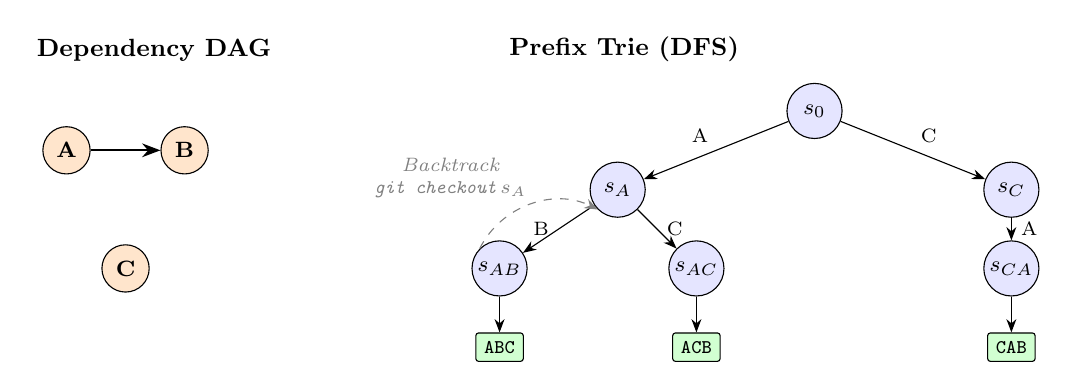
\begin{tikzpicture}[
  >=Stealth,
  every node/.style={font=\footnotesize},
  state/.style={draw, circle, inner sep=0.5pt, minimum size=7mm, fill=blue!10},
  leaf/.style={draw, rectangle, rounded corners=1pt, inner sep=3pt, fill=green!18, font=\scriptsize\ttfamily},
  depnode/.style={draw, circle, inner sep=1pt, minimum size=6mm, fill=orange!20, font=\footnotesize\bfseries},
]
% ---- Left panel: dependency DAG ----
\node[anchor=south west, font=\small\bfseries] at (-0.5, 3.5) {Dependency DAG};
\node[depnode] (dA) at (0, 2.5) {A};
\node[depnode] (dB) at (1.5, 2.5) {B};
\node[depnode] (dC) at (0.75, 1.0) {C};
\draw[->, thick] (dA) -- (dB);

% ---- Right panel: prefix trie ----
\node[anchor=south west, font=\small\bfseries] at (5.5, 3.5) {Prefix Trie (DFS)};
\node[state] (s0) at (9.5, 3.0) {$s_0$};
\node[state] (sA) at (7.0, 2.0) {$s_A$};
\node[state] (sC) at (12.0, 2.0) {$s_C$};
\node[state] (sAB) at (5.5, 1.0) {$s_{AB}$};
\node[state] (sAC) at (8.0, 1.0) {$s_{AC}$};
\node[state] (sCA) at (12.0, 1.0) {$s_{CA}$};
\node[leaf] (lABC) at (5.5, 0.0) {ABC};
\node[leaf] (lACB) at (8.0, 0.0) {ACB};
\node[leaf] (lCAB) at (12.0, 0.0) {CAB};
\draw[->] (s0) -- node[midway, above left=-1pt, font=\scriptsize] {A} (sA);
\draw[->] (s0) -- node[midway, above right=-1pt, font=\scriptsize] {C} (sC);
\draw[->] (sA) -- node[midway, left, font=\scriptsize] {B} (sAB);
\draw[->] (sA) -- node[midway, right, font=\scriptsize] {C} (sAC);
\draw[->] (sC) -- node[midway, right, font=\scriptsize] {A} (sCA);
\draw[->] (sAB) -- (lABC);
\draw[->] (sAC) -- (lACB);
\draw[->] (sCA) -- (lCAB);
% Backtrack annotation — arrow from sAB up to its parent sA, drawn
% above the nodes so it sits clear of the leaf row below.
\draw[->, dashed, gray] (sAB.north west) to[bend left=45] node[midway, above left=-1pt and -2pt, font=\scriptsize\itshape, gray, align=center] {Backtrack \\ \texttt{git checkout}\,$s_A$} (sA.south west);
\end{tikzpicture}
\caption{Reorder synthesis for a three-step window with one dependency edge ($A \to B$). The dependency graph on the left permits three valid orderings. The prefix trie on the right shows how shared prefixes are reused: the prefix $A$ is applied once, then reused by both orderings that begin with $A$.}
\label{fig:methodology-reorder-trie}
\end{figure}

\subsection{Manual-Refactor}
\label{sec:methodology-detector-manual}
\label{sec:methodology-manualrefactor}
\label{sec:arch-wrap-patch}

A \emph{Manual-Refactor} divergence point is emitted at any user step where (i) the action was performed by hand, and (ii) the resulting diff matches the structural pattern of an IDE-supported refactoring. IDE-driven refactorings arrive pre-tagged in the captured event stream, but a manual refactoring is just a series of edit bursts whose net effect happens to constitute a structured refactoring. The pipeline recovers them by running RefactoringMiner~\cite{alikhanifard2025rminer} -- a standard tool that detects refactorings between two code states by AST-level structural matching -- over a sliding window of commit pairs in the shadow repo. The window matters because a manual refactoring may unfold across several intermediate edit bursts, each of which on its own looks like an unrelated change; only by widening the window to cover the full span does the refactoring become visible to the miner. Each detected refactoring is then cross-checked against the captured event stream: a detection whose window contains a matching IDE-emitted refactoring event is recorded as IDE-driven, and one whose window contains no such event is flagged as manual. Adjacent candidate steps that share the same \texttt{(fromSha, toSha)} bracket are grouped into a single composite that the synthesiser treats as one refactoring.

\begin{figure}[H]
\centering
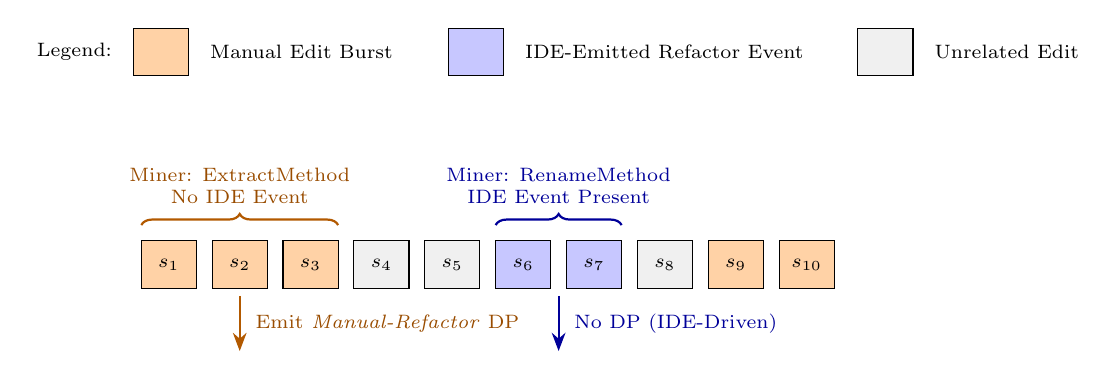
\begin{tikzpicture}[
  >=Stealth,
  every node/.style={font=\footnotesize},
  edit/.style={draw, rectangle, minimum width=7mm, minimum height=6mm, font=\scriptsize, fill=gray!12},
  manual/.style={edit, fill=orange!35},
  ide/.style={edit, fill=blue!22},
]
% Shift the trace and everything tied to it (braces, arrows, indicator
% text) right by 1.3, so the squares' midpoint coincides with the
% legend's natural midpoint and \centering puts the squares on the
% page midline. The legend itself stays at its original positions.
\begin{scope}[xshift=1.3cm]
% State sequence: s1..s3 manual extract; s4-s5 unrelated; s6-s7 IDE-driven rename; s8 unrelated; s9-s10 manual extract again
\node[manual] (s1) at (0.0, 0) {$s_1$};
\node[manual] (s2) at (0.9, 0) {$s_2$};
\node[manual] (s3) at (1.8, 0) {$s_3$};
\node[edit]   (s4) at (2.7, 0) {$s_4$};
\node[edit]   (s5) at (3.6, 0) {$s_5$};
\node[ide]    (s6) at (4.5, 0) {$s_6$};
\node[ide]    (s7) at (5.4, 0) {$s_7$};
\node[edit]   (s8) at (6.3, 0) {$s_8$};
\node[manual] (s9) at (7.2, 0) {$s_9$};
\node[manual] (s10) at (8.1, 0) {$s_{10}$};

% Window 1: t1..t3 — miner detects ExtractMethod
\draw[decorate, decoration={brace, amplitude=4pt}, thick, orange!70!black] (-0.35, 0.5) -- (2.15, 0.5)
  node[midway, above=4pt, font=\scriptsize, orange!60!black, align=center] {Miner: ExtractMethod \\ No IDE Event};
% Window 2: t6..t7 — miner detects RenameMethod, IDE event present
\draw[decorate, decoration={brace, amplitude=4pt}, thick, blue!60!black] (4.15, 0.5) -- (5.75, 0.5)
  node[midway, above=4pt, font=\scriptsize, blue!60!black, align=center] {Miner: RenameMethod \\ IDE Event Present};

% Result annotations below
\draw[->, thick, orange!70!black] (0.9, -0.4) -- (0.9, -1.1)
  node[midway, right=2pt, font=\scriptsize, orange!60!black] {Emit \emph{Manual-Refactor} DP};
\draw[->, thick, blue!60!black] (4.95, -0.4) -- (4.95, -1.1)
  node[midway, right=2pt, font=\scriptsize, blue!60!black] {No DP (IDE-Driven)};
\end{scope}

% Legend — placed above the two-line brace labels (which extend to y≈1.4),
% with each entry spaced out far enough in x that the text never reaches
% the next swatch.
\node[anchor=west, font=\scriptsize] at (-0.5, 2.7) {Legend:};
\node[manual] at (1.2, 2.7) {};
\node[anchor=west, font=\scriptsize] at (1.7, 2.7) {Manual Edit Burst};
\node[ide] at (5.2, 2.7) {};
\node[anchor=west, font=\scriptsize] at (5.7, 2.7) {IDE-Emitted Refactor Event};
\node[edit] at (10.4, 2.7) {};
\node[anchor=west, font=\scriptsize] at (10.9, 2.7) {Unrelated Edit};
\end{tikzpicture}
\caption{Manual-Refactor detection over a sliding edit window. RefactoringMiner detects structured refactorings between bracket endpoints, and each detection is checked against the IDE event stream. A detection with no matching IDE event is treated as manual and emits a divergence point; a detection with a matching IDE event is recorded as IDE-driven.}
\label{fig:methodology-manual-window}
\end{figure}

The manual-refactor synthesiser applies each detected refactoring spec through the corresponding IDE-style operation in JDT. It then runs a residual three-way merge to add back the user's other edits, such as bug fixes or small unrelated changes that were interleaved with the refactor. The resulting tree is committed to the shadow repository. This merge step is needed so that the alternative trajectory keeps the user's non-refactoring edits and still ends at the same code state as the original trajectory. The comparison then measures the difference between doing the refactoring by hand and doing it through the IDE, rather than being distorted by missing edits in the final state. Without this merge, the alternative trajectory would diverge from the user's final code and the process-score comparison would not be meaningful.

\paragraph{The wrap-and-patch layer.}
One practical issue is that sessions are recorded in IntelliJ, while the pipeline replays refactorings through JDT. The two engines can produce slightly different ASTs even when they are carrying out the same refactoring. To reduce these false divergences, the pipeline includes a wrap-and-patch layer between the JDT output and the validator. During testing, two recurring differences were observed. First, JDT adds the \texttt{static} modifier to an extracted method only when the method body requires it, whereas IntelliJ adds it whenever the body permits it. Second, JDT sometimes under-detects outer-scope-variable liveness in conditional branches, producing a void-returning method where IntelliJ produces a value-returning one. A host-side post-pass detects these patterns and rewrites the JDT output to match IntelliJ's structure. If a remaining difference cannot be patched safely, the bracket is marked as diverged and is not reordered. The wrap-and-patch layer therefore increases the number of usable brackets, but it does not cover every possible JDT-IntelliJ difference; full coverage is left as future work and discussed further in \S\ref{sec:methodology-validator}.

\subsection{Rework}
\label{sec:methodology-detector-rework}
\label{sec:methodology-reworksynth}

\emph{Rework} detection looks for edits that are later undone. In practice, this means finding content that is added and then removed, or removed and then added back, so that the two changes cancel out apart from whitespace. The detector parses each step's unified diff into hunks, maps each hunk to its enclosing method or class, and hashes the affected lines after normalising whitespace. It then greedily pairs added and removed hunks that share the same \texttt{(file, scope, content-hash)}. Each matched \texttt{(originating step, terminal step)} pair becomes a \emph{Rework} candidate, while pairs below the \emph{min\_rework\_lines} threshold are discarded as line-level noise.

\begin{figure}[H]
\centering
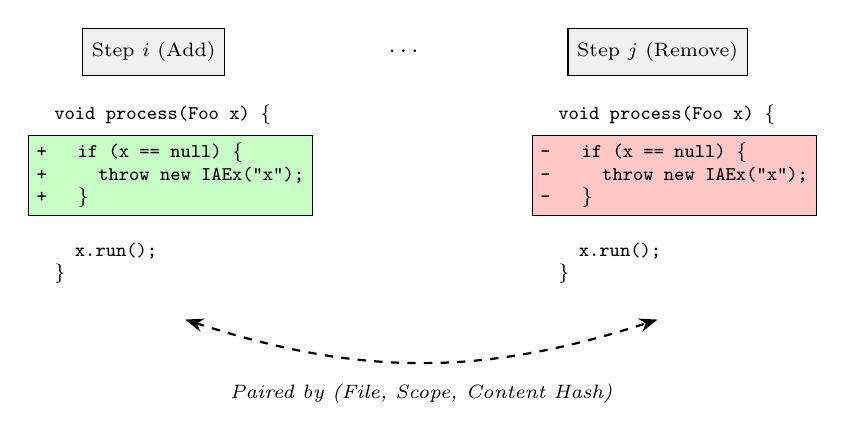
\begin{tikzpicture}[
  >=Stealth,
  every node/.style={font=\footnotesize},
  rstep/.style={draw, rectangle, minimum width=16mm, minimum height=6mm, font=\scriptsize, fill=gray!12},
]
% Step boxes on a timeline
\node[rstep] (si) at (0,0) {Step $i$ (Add)};
\node[font=\small] at (3.2, 0) {$\cdots$};
\node[rstep]      (sj) at (6.4,0) {Step $j$ (Remove)};

% --- step i column: context line above, green hunk box, context lines below ---
\node[anchor=north west, font=\ttfamily\scriptsize, align=left, inner sep=2pt]
  at (-1.6, -0.6)
  {\phantom{+} void process(Foo x) \{};
\node[draw, rectangle, fill=green!22, anchor=north west, font=\ttfamily\scriptsize, align=left, inner sep=3pt]
  (addbox) at (-1.6, -1.05)
  {\textbf{+} \quad if (x == null) \{\\
   \textbf{+} \qquad throw new IAEx("x");\\
   \textbf{+} \quad \}};
\node[anchor=north west, font=\ttfamily\scriptsize, align=left, inner sep=2pt]
  at (-1.6, -2.35)
  {\phantom{+} \quad x.run();\\
   \phantom{+} \}};

% --- step j column: same context, red hunk box ---
\node[anchor=north west, font=\ttfamily\scriptsize, align=left, inner sep=2pt]
  at (4.8, -0.6)
  {\phantom{-} void process(Foo x) \{};
\node[draw, rectangle, fill=red!22, anchor=north west, font=\ttfamily\scriptsize, align=left, inner sep=3pt]
  (rembox) at (4.8, -1.05)
  {\textbf{-} \quad if (x == null) \{\\
   \textbf{-} \qquad throw new IAEx("x");\\
   \textbf{-} \quad \}};
\node[anchor=north west, font=\ttfamily\scriptsize, align=left, inner sep=2pt]
  at (4.8, -2.35)
  {\phantom{-} \quad x.run();\\
   \phantom{-} \}};

% Pairing dashed connector — anchored below the full code column so the
% midway label sits clear of the bottom context lines on both sides.
\draw[<->, thick, dashed] (0.4, -3.4) to[bend right=18]
  node[midway, below=4pt, font=\scriptsize\itshape] {Paired by (File, Scope, Content Hash)}
  (6.4, -3.4);
\end{tikzpicture}
\caption{Rework detection for an added chunk that is later removed. The detector pairs the two hunks using their \texttt{(file, scope, content-hash)} tuple. The synthesiser then builds a shorter alternative trajectory by removing both halves of the rework and preserving the other intermediate edits.}
\label{fig:methodology-rework-pair}
\end{figure}

The rework synthesiser builds an alternative trajectory that skips the matched originating--terminal hunk pair. For each pair, it replays the $[\mathrm{originating}, \mathrm{terminal}]$ window as a sequence of small patches, leaving out the reworked chunk while preserving the other changes in the window. The replay is treated atomically: if any patch fails to apply, the whole alternative is discarded, so the system never scores a partially reconstructed trajectory.

A key issue is that the intermediate edits have shifted line numbers around the chunk. The terminal-step patch therefore has to translate its line coordinates from the user's tree, where the chunk reappears, to the synthesised tree, where the chunk was never written and the file may be several lines shorter. To do this, the synthesiser keeps a per-file drift tracker. It records the line offset between the two trees as a set of zones, and each intermediate user hunk shifts the zones after it by that hunk's net line change. This keeps each zone tied to the same logical content as the user's tree grows or shrinks around it.

After the reworked chunk is removed, some intermediate checkpoints no longer contain any substantive change: their only edit was the content that has now been omitted. Others contain only whitespace changes, such as blank-line edits around the removed chunk. Empty checkpoints are dropped from the alternative trajectory instead of being committed as no-op steps, while checkpoints whose remaining change is purely whitespace are folded into the preceding checkpoint. Both cases shorten the alternative's step count, which improves its process score through the step-savings term defined in \S\ref{sec:methodology-score}.

\subsection{Hygiene}
\label{sec:methodology-detector-hygiene}
\label{sec:methodology-hygiene}

\emph{Hygiene} detection covers two cases where the refactoring process remains technically valid but lacks a useful safety checkpoint. \emph{Tests-Skipped} is reported once for each 60-second composite window~\cite{murphyhill2009howrefactor} that contains at least one refactoring step but no successful test run. \emph{Commit-Gap} is reported once for each stretch of at least six green-refactor checkpoints, meaning checkpoints where the tests passed and the refactoring applied cleanly, without an intervening user commit. Each finding emits one divergence point.

The hygiene synthesiser builds alternatives in which the user ran tests or made a commit at the relevant checkpoint, without changing the code. For \emph{Tests-Skipped}, the alternative adds a synthetic \texttt{TEST\_RUN\_FINISHED} event at the anchor checkpoint. It does not change the recorded test outcome: \texttt{tests.success} and \texttt{tests.wasSkipped} remain as they were in the user's trace. The counterfactual is therefore ``the user should have run the tests here'', not ``the tests would have passed here''. This affects $W_{\textsc{st}}$, which depends on whether tests were run, but leaves $W_{\textsc{b}}$ unchanged because that term depends on the broken/passing outcome. For \emph{Commit-Gap}, the alternative adds a commit at the anchor checkpoint, breaking what would otherwise have been a long stretch of uncommitted green-refactor checkpoints.

In both cases, the alternative changes only the process metadata at the anchor checkpoint, not the code. This is because hygiene concerns the process around the refactoring: when tests were run and when commits were made. Synthesis therefore amounts to flipping the relevant process flag at the anchor checkpoint and feeding the trajectory back through Phase B (\S\ref{sec:arch-phases}). The difference between the original and adjusted final scores gives the process-score cost of the skipped hygiene event.

\subsection{Validator and behaviour preservation}
\label{sec:methodology-validator}

The bracket-level validator checks whether the user's specs can be replayed in order to reach the same final state as the user's trajectory. For each \texttt{(fromSha, toSha)} bracket, it replays the specs and then applies two checks. First, the set of changed \texttt{.java} files must match \texttt{git diff fromSha..toSha}. Second, the terminal AST hash for each changed file must match the user's version. Brackets that pass both checks are marked as \emph{valid} and can be used as reorder windows. Brackets that fail are split into individual steps and are not reordered. The replay uses the same borrowed worktree and JDT batch-session machinery as the reorder engine (\S\ref{sec:arch-reorder-engine}).

The number of brackets that pass validation is limited by differences between JDT and IntelliJ, as discussed in \S\ref{sec:arch-wrap-patch}. If the wrap-and-patch layer covers the difference, the bracket can still be marked as valid. If it does not, the bracket fails validation even when the original refactoring was correct. Covering all structural differences between JDT and IntelliJ is left as future work, and this limitation is the main reason \emph{Ordering} recall is not higher in \S\ref{sec:results-divergence}.

\section{System architecture and pipeline phases}
\label{sec:arch-phases}

This section describes the four JVM modules that make up the tool and explains how they fit into the analysis pipeline. \S\ref{sec:arch-overview} gives the module-level overview and dataflow, while \S\ref{sec:methodology-phases-split} explains the Phase A / Phase B split used by the implementation.

\subsection{Architecture at a glance}
\label{sec:arch-overview}

The tool is split into four JVM modules (\texttt{:ide-plugin}, \texttt{:analysis}, \texttt{:refactoring-bundle}, and \texttt{:shared}) and a separate React/TypeScript dashboard (\texttt{dashboard/}):

\begin{itemize}
  \item \texttt{ide-plugin/} -- an IntelliJ plugin that records the developer's session as a stream of typed events and uploads it to the analysis server. The user starts and stops recording with a button in the IDE.
  \item \texttt{analysis/} -- the Kotlin analysis pipeline. It ingests recorded sessions, reconstructs a shadow git repository, mines and synthesises trajectories, computes per-checkpoint metrics, and emits an \texttt{AnalysisReport}.
  \item \texttt{refactoring-bundle/} -- a headless Eclipse JDT distribution wrapped in an embedded Equinox OSGi framework. The analysis module calls into it across the OSGi class\-loader boundary (details in \S\ref{sec:arch-wrap-patch}).
  \item \texttt{dashboard/} -- a React/TypeScript single-page app that renders the \texttt{AnalysisReport} (details in \S\ref{sec:arch-dashboard}).
\end{itemize}

Figure~\ref{fig:arch-overview} summarises the dataflow between these components.

\begin{figure}[H]
\centering
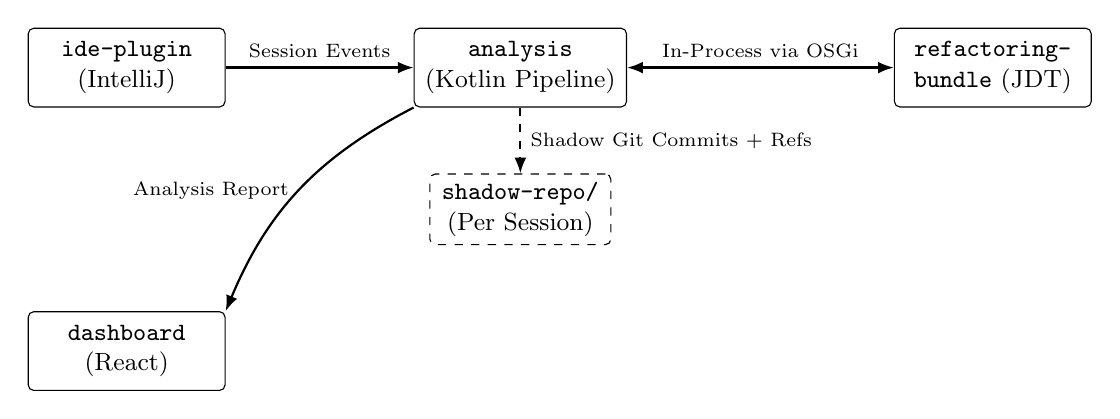
\begin{tikzpicture}[
  font=\small,
  box/.style={draw, rounded corners=2pt, minimum width=2.5cm, minimum height=1.0cm, align=center, inner sep=4pt},
  shadow/.style={draw, dashed, rounded corners=2pt, minimum width=2.3cm, minimum height=0.8cm, align=center, inner sep=3pt},
  arrow/.style={-{Latex[length=2mm]}, thick},
  dasharrow/.style={-{Latex[length=2mm]}, thick, dashed},
  biarrow/.style={{Latex[length=2mm]}-{Latex[length=2mm]}, thick},
]

  \node[box] (plugin) at (0, 0) {\texttt{ide-plugin}\\(IntelliJ)};
  \node[box] (analysis) at (5, 0) {\texttt{analysis}\\(Kotlin Pipeline)};
  \node[box] (bundle) at (11, 0) {\texttt{refactoring-}\\\texttt{bundle} (JDT)};

  \node[shadow] (shadow) at (5, -1.8) {\texttt{shadow-repo/}\\(Per Session)};

  \node[box] (dashboard) at (0, -3.6) {\texttt{dashboard}\\(React)};

  \draw[arrow] (plugin) -- node[above, font=\scriptsize] {Session Events}
                                (analysis);
  \draw[biarrow] (analysis) -- node[above, font=\scriptsize] {In-Process via OSGi}
                                  (bundle);

  \draw[dasharrow] (analysis) -- node[right, font=\scriptsize] {Shadow Git Commits + Refs} (shadow);

  \draw[arrow] (analysis.south west) to[bend right=20]
                                  node[left, font=\scriptsize, pos=0.5] {Analysis Report}
                                  (dashboard.north east);

\end{tikzpicture}
\caption{High-level dataflow through the tool. The IDE plugin records the session, the analysis pipeline reconstructs and scores the trace, and the embedded JDT bundle applies synthesised refactorings. The dashboard displays the resulting report, while the shadow repository stores user checkpoints and synthesised alternatives as per-session git commits.}
\label{fig:arch-overview}
\end{figure}

\subsection{Phase A / Phase B split}
\label{sec:methodology-phases-split}

The detector and synthesisers above run as part of an offline analysis pipeline. The pipeline is split into two phases, with \texttt{PhaseAResult} acting as the serialisable boundary between them.

\paragraph{Phase A.}
Phase A performs the expensive work: ingesting and normalising events, reconstructing the shadow repository, mining refactorings, running the four synthesisers and the validator, computing per-checkpoint metrics, and tracking PMD / CPD findings across checkpoints. It usually takes minutes per session. Most of that time comes from the per-checkpoint Gradle builds and JUnit runs described in \S\ref{sec:arch-metrics}, plus the Equinox-hosted JDT refactoring calls described in \S\ref{sec:arch-jdt}. The output is a \texttt{PhaseAResult}. This contains the reconstructed trace, mined steps and typed refactoring specs, metrics for the user's trajectory and each synthesised alternative SHA, the diff bundle, PMD / CPD tracking edges, and the generated reorder trajectories.

\paragraph{Phase B.}
Phase B takes the \texttt{PhaseAResult} and a \texttt{ScoringConfig}, which contains the six process-score weights from \S\ref{sec:methodology-weights}. It then runs the \texttt{ReportAssembler}. This computes the process score, clamps it to the [0,100] range, attaches alternative-vs-user deltas at each checkpoint, and emits the final \texttt{AnalysisReport}. Unlike Phase A, Phase B does not touch the filesystem, run JDT, or execute tests. It only walks the cached data in memory, so it finishes in milliseconds.

This split matters because the weights are only used in Phase B. Changing them does not invalidate the cached Phase A results. The sensitivity experiment in Chapter~\ref{ch:results} uses this property directly: $12 \times 9 \times 45 = 4{,}860$ scoring configurations are evaluated against the same cached set of \texttt{PhaseAResult} dumps in roughly $2.6$ seconds of wall-clock time, because each configuration only re-runs \texttt{ReportAssembler}. The CLI exposes the split through two Gradle entrypoints: \texttt{:analysis:phaseA} writes a \texttt{PhaseAResult} JSON file to disk, and \texttt{:analysis:phaseB} reruns the cheap second phase using a Phase A dump and a chosen \texttt{ScoringConfig}.

\section{Dashboard}
\label{sec:arch-dashboard}

The detector and synthesisers produce an analysis report, and the dashboard presents that report to participants. The dashboard is a React web app hosted inside the IDE through JCEF, IntelliJ's embedded Chromium browser, in a dialog rather than a separate browser page, and the plugin passes the completed report to the page once analysis has finished. Figure~\ref{fig:arch-dashboard} shows the dashboard in use on one of the user-study sessions.

The main view is a trajectory chart showing the user's process score over time, with synthesised alternatives overlaid for comparison. Participants can toggle the individual code-cleanliness signals on the chart, such as readability, complexity, duplication, code smells, coupling, and cohesion, to see how different aspects of the code changed across the session. Selecting a step opens a detail panel for the exact edit made at that point, including the affected code, the metrics that changed, and any divergence point associated with the step. Divergence points are clickable: they explain what went wrong, what alternative action the developer \emph{could} have taken, and how much that alternative would have changed the process score. The dashboard also surfaces the locations of code smells and duplicated code, and shows build and test status over time so participants can see where the session became broken and where it recovered. It also highlights the highest-impact and actionable takeaways from the session as a whole.

\begin{figure}[htbp]
  \centering
  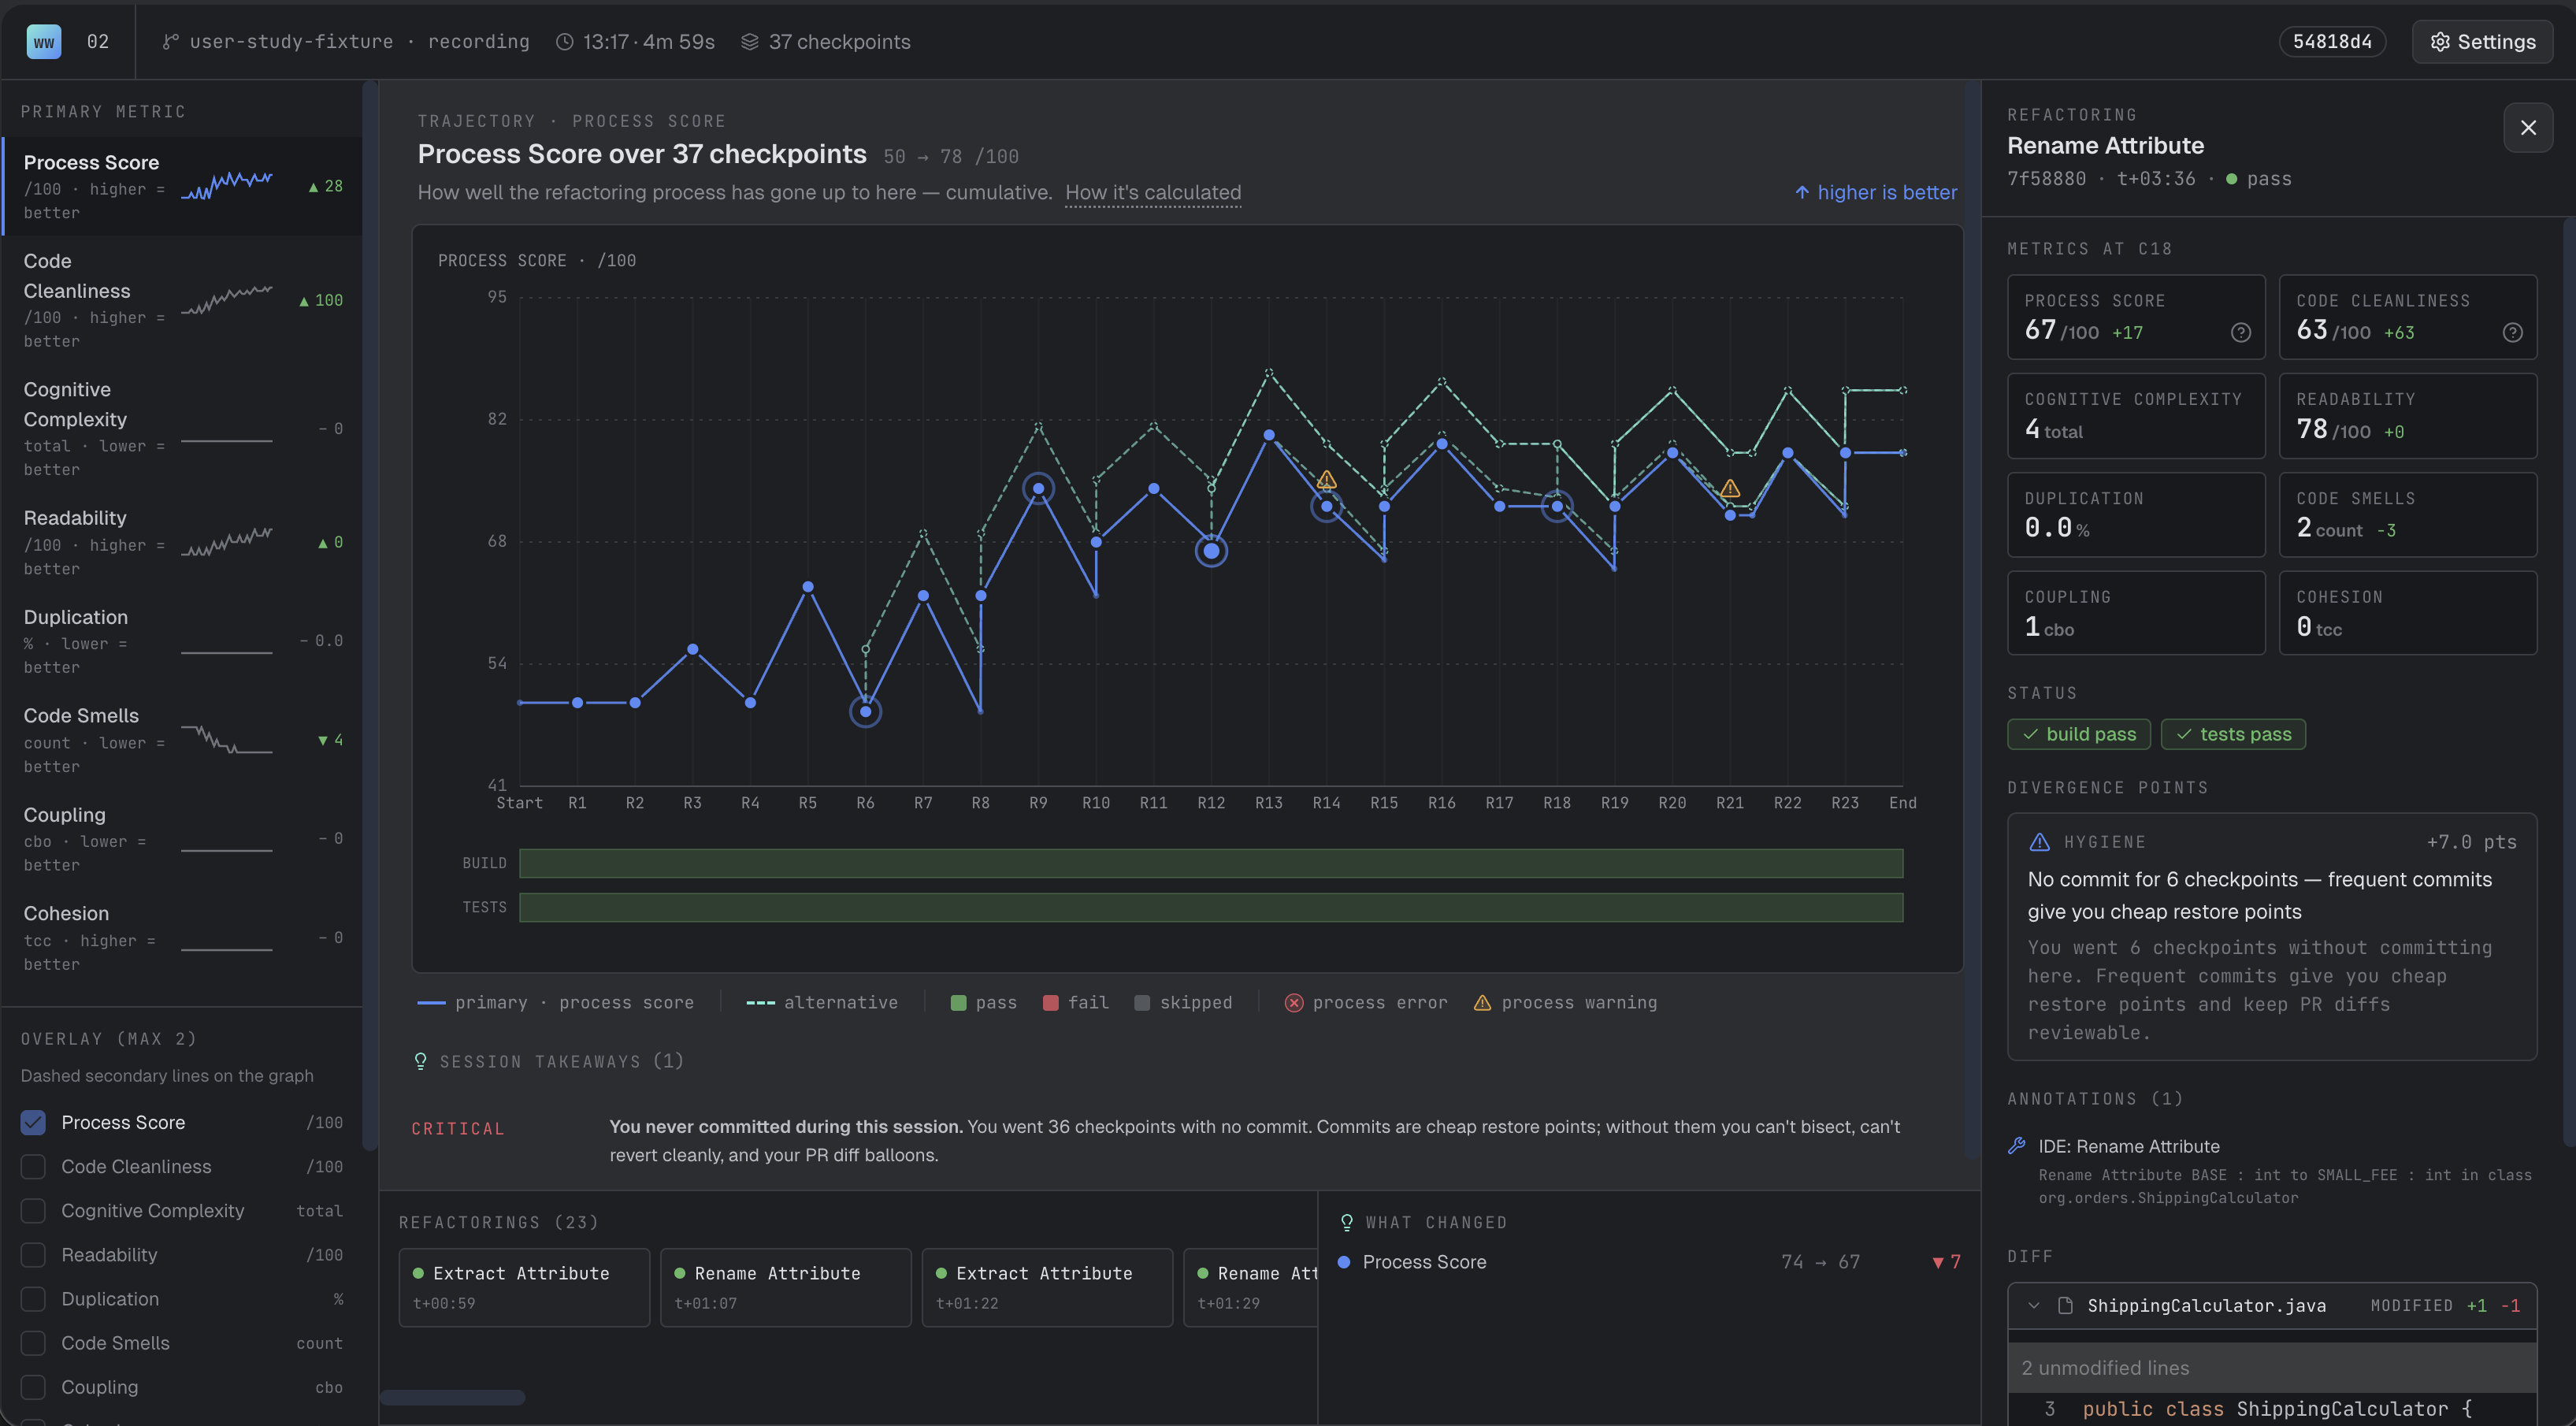
\includegraphics[width=\textwidth]{architecture/dashboard_image.png}
  \caption{The dashboard hosted inside an IntelliJ JCEF window. The centre chart plots the user's process score across the session and can overlay alternative trajectories and individual cleanliness signals. The side panels show the selected step, metric changes, build/test status, smell and duplication locations, and any divergence point associated with that step, including the suggested alternative and its score impact. The lower panel summarises the highest-impact takeaways for the session.}
  \label{fig:arch-dashboard}
\end{figure}

\section{Score-formula evaluation design}
\label{sec:methodology-score-eval}

The results chapter evaluates the score formula in two ways. The first asks whether the ranking of divergence points is stable when the weights are perturbed. The second asks whether the individual terms in the formula actually contribute to the magnitudes the detector reports. This section defines the shared experimental procedure for those tests; Chapter~\ref{ch:results} reports the observed numbers.

\subsection{Sensitivity perturbations}
\label{sec:methodology-sensitivity-design}

The sensitivity experiment compares the ranking of divergence points computed by the production weights with rankings produced under perturbed weights. Two perturbation schemes are used. In the single-knob sweep, one weight is varied while all other weights remain at their production values. In the multi-knob sweep, all weights are varied at once by drawing independent log-normal scale factors. For weight $W_i$, the sampled value is
\[
W'_i = W_i \cdot \exp(\sigma Z_i),
\]
where $Z_i \sim \mathcal{N}(0, 1)$ and $\sigma = \ln 2$. This makes the perturbation symmetric in log-space: multiplying and dividing by the same factor are treated as equally large changes, and most samples remain within a few multiples of the production value.

Ranking stability is measured with Kendall's $\tau$-b~\cite{kendall1948rank,agresti2010ordinal} and top-$N$ hit rate. Kendall's $\tau$-b is used because the rankings are short and may contain ties. A value of $\tau = 1.0$ means the perturbed ranking is unchanged, while $\tau < 0$ means the order has mostly inverted. Top-$N$ hit rate asks how many of the production top-$N$ divergence points remain in the perturbed top-$N$. Top-$1$ is the main comparison because it is defined for any session with at least one divergence point; larger $N$ values are only informative for sessions with enough surfaced points. Ties are broken by ascending step index so that production and perturbed rankings are compared deterministically.

\subsection{Ablation design}
\label{sec:methodology-ablation-design}

The ablation experiment tests whether the score formula depends on each of the seven non-sub-cleanliness terms: gain, broken-build time, skipped tests, manual-when-IDE, length, lag, and commit gap. It enumerates subsets of these process weights, keeps the selected terms at their production values, and sets the others to zero. Since there are seven non-sub-cleanliness terms, the full power set contains $2^7 = 128$ variants, which is small enough to enumerate exactly. This follows the same logic as composite-indicator sensitivity analysis~\cite{saisana2005composite} and exact Shapley-style feature attribution when the number of features is small~\cite{lundberg2017shap,strumbelj2014explaining}.

Two recovery measures are used to describe how much divergence-point magnitude remains under an ablated formula. Mean recovery computes the recovery ratio per fixture and averages those ratios. Sum-over-sum recovery instead sums $\lvert\mathrm{magnitude}\rvert$ across all divergence points in all fixtures and divides by the same sum under the production formula. Sum-over-sum is treated as the main measure because it avoids giving empty or near-empty fixtures the same weight as fixtures with many surfaced divergence points. The ablation also reports Kendall's $\tau$-b so that magnitude loss and ranking change can be considered separately.

\section{Evaluation dataset and labelling protocol}
\label{sec:methodology-rater}

The experiments in Chapter~\ref{ch:results} use a set of $45$ refactoring sessions that we recorded by hand on a Java library-style fixture in IntelliJ. This section explains how the sessions were assembled, how they were labelled, and how the labels were checked by raters.

The IDE-event capture literature surveyed in \S\ref{sec:process-aware-logging} shows that detailed development traces can be collected. However, we did not find an existing dataset that combines per-event code content with IDE-side refactoring events for Java sessions recorded in IntelliJ. This matters for the IDE-versus-manual signal. RefactoringMiner can recover a structural refactoring from a pair of code states, but it cannot tell whether the developer used the IDE refactoring command or typed the change by hand. Since that distinction is part of the manual-when-IDE penalty in \S\ref{sec:methodology-score}, it has to be captured at recording time.

The evaluation also needs controlled examples of the behaviours the detector is meant to find. The precision and recall results in \S\ref{sec:results-divergence} are computed against sessions where a specific process issue was deliberately introduced. A free-form session dataset would not provide that controlled injection signal directly. For these reasons, we recorded our own dataset using the IntelliJ plugin described in \S\ref{sec:arch-events}, so that IDE events were captured as the sessions happened.

\subsection{The 45-session injection set}
\label{sec:methodology-injection-set}

Each session follows a scripted playbook scenario designed to trigger one specific kind of process issue. Examples include choosing a less favourable order for a set of refactoring steps, undoing and redoing the same chunk of code, skipping the expected test cadence, or making a manual edit where an IDE refactoring would have applied. The playbook covers all four divergence kinds: $5$ sessions target ordering, $9$ target rework, $13$ target hygiene, and the remaining sessions are split between IDE-replay injections and clean controls where no issue is deliberately introduced.

\subsection{Two label streams}
\label{sec:methodology-labels}

Each session has two kinds of label, because the evaluation asks two slightly different questions. The first label records the divergence kind that was deliberately injected into the session, i.e. the behaviour the playbook was designed to trigger. This is used for the \emph{injection prominence} analysis in \S\ref{sec:results-divergence}. The second label is a separate hand-written set of all divergence kinds that should be detected in the session. This label can contain more than one kind, because a session designed to trigger one issue may also legitimately contain another. The per-kind precision and recall results in \S\ref{sec:results-divergence} use this second label set, and its inter-rater agreement is reported in \S\ref{sec:results-kappa}.

The multi-label schema uses the four divergence kinds $\mathcal{K} = \{\emph{IDE-Replay}, \emph{Rework}, \emph{Hygiene}, \emph{Ordering}\}$ and each session is allowed to have more than one expected kind. For example, a session may contain both an ordering divergence and a hygiene flag.

\subsection{Rater protocol}
\label{sec:methodology-rater-protocol}

To check the schema independently, two annotators, denoted P1 and P2 in the results chapter, labelled all $45$ sessions using the same schema. They completed this labelling before either of them took part in a user-study session. Each rater received the schema definition and the raw artefacts for every recording: the event log \texttt{events.jsonl} and the session metadata \texttt{session.json}. They did not receive the playbook prompts, our \texttt{manifest-v2.csv} labels, the Phase A \texttt{analysis-report.json}, or access to the dashboard. This kept the hand labels separate from both the injected labels and the detector output.

The event log stores the full file contents after each event rather than a compact diff. To make the sessions easier to inspect, raters were also given a small read-only helper script, \texttt{tool/scripts/session-event-diffs.py}, which prints a unified diff for each \emph{edit\_burst} and \emph{refactoring\_finished} event. The script is only helps to present the information from the events to the users in a more readable format and does not expose any extra information: it derives its output from the same \texttt{events.jsonl} file already given to the raters.

\subsection{Cohen's $\kappa$ computation}
\label{sec:methodology-kappa}

Agreement is reported with Cohen's $\kappa$~\cite{cohen1960kappa}, computed separately for each divergence kind in $\mathcal{K}$. For a given kind $k$, each session is treated as a binary judgement: either $k$ is present in \texttt{expected\_kinds}, or it is not. This gives a $2 \times 2$ table for each rater pair, from which $\kappa$ is computed. The results are interpreted using the Landis and Koch thresholds~\cite{landis1977kappa}: $\kappa < 0.20$ is slight agreement, $0.21$--$0.40$ fair, $0.41$--$0.60$ moderate, $0.61$--$0.80$ substantial, and $0.81$--$1.00$ almost perfect. Because the dataset contains only $45$ sessions, the raw agreement counts from each table are reported alongside $\kappa$; at this size, the yes/yes, no/no, and disagreement counts are still useful to inspect directly.

\subsection{Treatment of disagreements}
\label{sec:methodology-disagreements}

Disagreements are reported as part of the study rather than resolved by changing our labels or the raters' labels. When both raters agree with each other but disagree with our label, as with rework in session 043, the session is named explicitly in the results chapter and treated as a case where our label may be the outlier.

The rater-study results, including the per-kind $\kappa$ values, raw agreement counts, and disagreement patterns, are reported in Table~\ref{tab:results-userstudy-kappa} (\S\ref{sec:results-kappa}).

\subsection{Divergence-detector evaluation protocol}
\label{sec:methodology-detector-eval}

The divergence-detector experiment runs the full analysis pipeline on each of the $45$ recorded sessions using the production score weights. For each session, the detector output is compared with the session's \texttt{expected\_kinds} label. A true positive means that the detector surfaced at least one divergence point of the expected kind somewhere in the session, a false negative means that an expected kind was not surfaced, and a false positive means that the detector surfaced a kind not present in \texttt{expected\_kinds}. Matching is done at the session level rather than against an exact recorded step, because step boundaries depend on the plugin's edit-burst flushing and are not stable enough to treat as ground truth.

Precision and recall are reported separately for each kind. They are not collapsed into F1 or accuracy because the two error types have different practical meanings: a false positive shows the user an alternative that should not be there, while a false negative means the dashboard missed a useful opportunity. Accuracy is also uninformative because most kind-by-session cells are true negatives.

The experiment also checks whether the detector's output would be useful to a user. The first check is whether a surfaced alternative genuinely beats the user's trajectory, using the strict condition $\mathrm{magnitude} > 0$ under the trajectory-final score definition in \S\ref{sec:methodology-detector}. The second is injection prominence: for the divergence kind deliberately introduced by the playbook, the experiment records whether the corresponding positive-magnitude divergence point is the highest-ranked point in that session.

\chapter{Experimentation and Evaluation}
\label{ch:results}

This chapter evaluates the score formula, the divergence-point detector, and the use of their feedback in complete refactoring sessions. The formula is tested through sensitivity and ablation experiments, the detector against labelled injection sessions, and the end-to-end workflow through a 30-session human study plus an agent extension on the same codebase.

\S\ref{sec:results-metric} reports the score-formula experiments. \S\ref{sec:results-detector} reports detector precision and recall against externally labelled divergence kinds. \S\ref{sec:results-studies} reports the human and agent studies, where the outcome is whether feedback is reflected in later refactoring behaviour.

The labelled detector experiment uses the 45-session injection set and two-label scheme defined in \S\ref{sec:methodology-rater}. Because the per-kind counts are small, tables report raw counts alongside percentages. Every magnitude value in this chapter is the trajectory-final $J$ delta defined in \S\ref{sec:methodology-score}, so magnitudes are comparable across the four divergence kinds.

\section{Testing the score formula}
\label{sec:results-metric}

The score weights were chosen from a literature-supported severity ordering (\S\ref{sec:methodology-weights}), not fitted to an external outcome dataset. This section therefore tests whether the rankings are stable under plausible weight changes and whether the seven process-side terms contribute measurable signal, following the evaluation design in \S\ref{sec:methodology-score-eval}. \S\ref{sec:results-headline} then reports a structural limit of the formula that appears in both experiments.

\subsection{Sensitivity sweep}
\label{sec:results-sensitivity}

The first experiment measures how sensitive the divergence-point ranking is to the weights in the process-score formula. Large ranking changes under small weight perturbations would indicate that the reported priorities depend too strongly on arbitrary parameter choices. The experiment uses the single-knob and multi-knob perturbation methods defined in \S\ref{sec:methodology-sensitivity-design}. The main result is that the top-ranked divergence point is usually stable across all three session sets, although some terms do affect the ranking in identifiable cases.

\paragraph{Experiment setup.}
For the single-knob sweep, the chosen weight is scaled by one of nine factors in $\{0.1, 0.25, 0.5, 0.75, 1.25, 1.5, 2.0, 4.0, 10.0\}$. With twelve weights ($6$ process-side and $6$ cleanliness-side), this gives $12 \times 9 \times \lvert \mathcal{C} \rvert$ perturbation runs per session set $\mathcal{C}$. The multi-knob sweep draws $200$ independent samples per session using the log-normal sampling scheme defined in \S\ref{sec:methodology-sensitivity-design}.

The experiment is run against three session sets: the $45$ hand-labelled injection sessions of \S\ref{sec:results-divergence}, the $30$ user-study sessions of \S\ref{sec:results-userstudy}, and the $48$ agent extension sessions of \S\ref{sec:results-userstudy-agent}. These differ in their per-session divergence-point profiles. The injection sessions have at most $5$ divergence points per session and concentrate on single-kind exercises. The user-study sessions have up to $13$ per session across naturalistic sessions ($121$ in total, mean $4.0$ per session, with the no-feedback baseline arm carrying most of the high-count sessions). The agent sessions have at most $3$ per session across the eight agent stacks ($42$ in total, mean $0.9$ per session), consistent with the structural detector biases against agent edit patterns discussed in \S\ref{sec:results-userstudy-agent}.

As defined in \S\ref{sec:methodology-sensitivity-design}, ranking stability is reported using Kendall's $\tau$-b and top-$N$ hit rate. Top-$1$ is the only metric that works across all three session sets, since it applies to any session with at least one divergence point. Top-$3$ and top-$5$ are reported on the user-study sessions only, where the per-session rankings are large enough to make them informative. Several divergence-point kinds produce ties, so ties are broken by ascending step index in both the production and perturbed rankings.

\paragraph{Single-knob results.}
Table~\ref{tab:results-sensitivity-headline} reports top-$1$ stability across the three session sets. The user-study sessions are the most demanding test: they have the longest per-session rankings, the highest divergence-point density, and the lowest baseline saturation. The injection sessions show the highest top-$1$ stability, but only because the per-session rankings are shorter and offer less surface area to reshuffle. The agent sessions sit between them, and $17.5\%$ of their baseline divergence points hit the score-clamp ceiling, which suppresses the observable effect of weight perturbations on a non-trivial slice of the agent set. On the user-study sessions the top-$1$ recommendation is preserved on $3{,}141$ of $3{,}240$ rows ($96.9\%$).

\begin{table}[htbp]
\centering
\small
\begin{tabular}{lrrrrr}
\hline
\textbf{session set} & \textbf{rows} & \textbf{$\tau = 1.0$} & \textbf{top-$1$ $= 1$} & \textbf{$\tau < 0$} & \textbf{baseline saturation} \\
\hline
Injection ($45$)         & $4{,}860$ & $77.0\%$ & $99.8\%$ & $0.3\%$ & $10.6\%$ \\
\textbf{User study ($30$)} & $3{,}240$ & $51.5\%$ & $\mathbf{96.9\%}$ & $0.8\%$ & $\mathbf{6.4\%}$ \\
Agent ($48$)              & $5{,}184$ & $88.5\%$ & $98.5\%$ & $1.2\%$ & $17.5\%$ \\
\hline
\end{tabular}
\caption{Single-knob sensitivity across three session sets. The user-study sessions are the discriminating benchmark: longest per-session rankings and lowest baseline saturation. The $\tau = 1.0$ share is meaningfully lower on the user-study set ($51.5\%$) than on the injection set ($77.0\%$) or the agent set ($88.5\%$) because user-study rankings are long enough to allow tail reshuffling under arbitrary single-knob perturbation, even when the top-of-ranking decision is preserved on $96.9\%$ of rows.}
\label{tab:results-sensitivity-headline}
\end{table}

\paragraph{Sources of ranking instability.}
Table~\ref{tab:results-sensitivity-knobs} reports per-knob top-$1$ disruption counts on the user-study sessions. Every process-side weight produces measurable disruption between $4.4\%$ and $8.9\%$ of rows; the six cleanliness sub-weights produce at most $0.7\%$ disruption each, with three of them producing none at all. The largest disruptor is the cleanliness-gain weight $W_{\textsc{g}}$ ($24$ of $270$ rows, $8.9\%$), followed by the manual-when-IDE weight $W_{\textsc{mi}}$ ($17$ rows), the skipped-tests weight $W_{\textsc{st}}$ ($15$), and the commit-gap weight $W_{\textsc{cg}}$ ($15$). The length-bonus and broken-build weights are close behind ($14$ and $12$). The decomposition tells us the score formula's \emph{effective parameter dimension} is closer to six (the process-side terms) than to twelve: the cleanliness composite usually adds the same amount to both paths so it does not change the ranking, and the process-side weights do almost all of the rank-shaping.

\begin{table}[htbp]
\centering
\small
\begin{tabular}{lrr}
\hline
\textbf{knob} & \textbf{top-$1$ disruptions / $270$ rows} & \textbf{share} \\
\hline
\texttt{gain}        & $24$ & $8.9\%$ \\
\texttt{manualIde}   & $17$ & $6.3\%$ \\
\texttt{skipTests}   & $15$ & $5.6\%$ \\
\texttt{commitGap}   & $15$ & $5.6\%$ \\
\texttt{length}      & $14$ & $5.2\%$ \\
\texttt{broken}      & $12$ & $4.4\%$ \\
\hline
\multicolumn{3}{l}{\textit{cleanliness sub-weights: \texttt{coupling} $2$ ($0.7\%$), \texttt{smells} $1$, \texttt{cohesion} $1$, all others $0$}} \\
\hline
\end{tabular}
\caption{Per-knob top-$1$ disruption counts on the user-study sessions (30 sessions $\times$ 9 perturbation factors $=$ 270 rows per knob). The six process-side weights account for almost every top-$1$ shift; cleanliness sub-weights produce at most $0.7\%$ disruption each. The cleanliness-gain weight $W_{\textsc{g}}$ is the most leverage-y single knob on this corpus.}
\label{tab:results-sensitivity-knobs}
\end{table}

\paragraph{Multi-knob Monte Carlo.}
The single-knob sweep only tests one weight at a time. The multi-knob Monte Carlo perturbs every weight together. Table~\ref{tab:results-sensitivity-mc} reports the distribution of $\tau$ and top-$N$ hit rate across $200 \times \lvert \mathcal{C} \rvert$ joint-perturbation samples per session set.

The multi-knob result is meaningfully weaker than the single-knob headline. On the user-study sessions, the top-$1$ recommendation changes on $13.1\%$ of joint-perturbation samples, against $3.1\%$ under single-knob, and mean $\tau$ falls to $0.656$. The injection sessions are more stable on top-$1$ ($99.1\%$) but their multi-knob mean $\tau$ falls to $0.805$, comparable in magnitude to the user-study drop, because joint perturbation can reshuffle long stretches of the tail even when the highest-magnitude divergence point is preserved. The agent sessions sit between the two on mean $\tau$ ($0.848$), with top-$1$ stability at $92.6\%$. The formula is robust to small joint perturbations and degrades smoothly with larger ones. It is not robust to arbitrary combinations of weights, even within the realistic range we tested.

\begin{table}[htbp]
\centering
\small
\begin{tabular}{lrrrrr}
\hline
\textbf{session set} & \textbf{samples} & \textbf{mean $\tau$} & \textbf{top-$1$ $= 1$} & \textbf{top-$3$ $= 1$} & \textbf{top-$5$ $= 1$} \\
\hline
Injection ($45$)         & $9{,}000$ & $0.805$ & $99.1\%$ & $77.8\%$ & $77.8\%$ \\
\textbf{User study ($30$)} & $6{,}000$ & $\mathbf{0.656}$ & $\mathbf{86.9\%}$ & $\mathbf{68.0\%}$ & $66.6\%$ \\
Agent ($48$)              & $9{,}600$ & $0.848$ & $92.6\%$ & $91.0\%$ & $89.6\%$ \\
\hline
\end{tabular}
\caption{Multi-knob Monte Carlo robustness across three session sets ($200$ samples per session, log-normal $\sigma = \ln 2$). The user-study sessions are the discriminating benchmark; the multi-knob top-$1$ stability is $\sim 10$ percentage points lower than the single-knob result on the same set. Top-$3$ and top-$5$ track top-$1$ on the agent set ($91.0\%$ and $89.6\%$) but drop substantially on the user-study set ($68.0\%$ and $66.6\%$) where per-session rankings are longer and the tail is more reshuffleable.}
\label{tab:results-sensitivity-mc}
\end{table}

\paragraph{Saturation and score-clamp bias.}
One concern is whether the $\tau$ and top-$N$ numbers reflect the $[0, 100]$ clamp on the process score rather than true stability. When both user and alt scores hit the ceiling, their magnitude is zero regardless of weights, which would inflate $\tau$. Saturation is therefore tracked per session. The right-hand column of Table~\ref{tab:results-sensitivity-headline} shows the three session sets differ substantially. The injection sessions have $10.6\%$ saturated baseline divergence points, concentrated on the short single-kind sessions. The agent sessions have $17.5\%$, because many agent sessions push the score close to the ceiling on the easier playbook sessions (the S4 no-op session in particular runs at $J = 45$ across every agent cell). The user-study sessions sit lowest at $6.4\%$. The user-study set is therefore the cleanest benchmark for the perturbation statistics: its $\tau$ and top-$N$ values are dominated by real perturbation response rather than clipping artefacts.

\paragraph{Caveats and scope.}
Three main limitations. First, the experiment establishes that the formula is stable near the production weights. It does not establish that the production weights themselves are uniquely correct, only that small changes to them mostly preserve the ranking. To properly validate this, we'd need to refit the weights against an external outcome dataset, e.g.\ longitudinal code-quality measurements, but no such dataset exists for this problem. Second, the multi-knob test is centred around the production weights and covers the neighbourhood within roughly $\pm 2\sigma$ (about $\times 0.25$ to $\times 4$). The formula visibly degrades on the user-study sessions even inside this range ($\tau = 0.656$ mean), so the robustness claim is local rather than global. Third, the user-study sessions are $n = 30$ across $5$ participants split into a with-feedback arm ($n = 3$) and a no-feedback baseline arm ($n = 2$); both arms feed the robustness corpus on the basis that they exercise the same scoring formula on the same codebase. We document these limits as threats to validity in \S\ref{sec:results-scoped-out} and the discussion chapter. The chapter does not claim more than the experiments support.

\subsection{Ablation sweep}
\label{sec:results-ablation}

The sensitivity sweep shows the ranking is robust to weight perturbations. This experiment asks the different question of whether every term in the score formula carries substantial weight. Using the ablation design defined in \S\ref{sec:methodology-ablation-design}, the experiment enumerates all $2^7 = 128$ subsets of the seven process-side weights (including the intermediate-cleanliness lag weight $W_{\textsc{lag}}$), producing $5{,}760$ rows across the $45$ injection sessions. The cleanliness sub-weights are kept at production because the sensitivity sweep showed that perturbing them almost never reshuffles the ranking; ablating them would inflate the variant count from $128$ to $8{,}192$ for little additional information. The sweep rules out two failure modes: sum-over-sum recovery rises from exactly $0.000$ when every process term is zeroed to $1.000$ under the full formula, and mean $\tau$ rises in parallel from $0.744$ to $0.833$.

\paragraph{Sanity check.}
The full-formula variant (all seven terms active) reproduces production exactly: $\tau = 0.833$ (set by the saturation floor on the injection set, not by ablation), recovery $= 1.000$, and mean $\lvert \Delta \textnormal{magnitude} \rvert = 0.000$ on every session. Comparison and production use the same system.

\paragraph{Monotone by active-term count.}
Table~\ref{tab:results-ablation-monotone} groups the $5{,}760$ rows by how many process-score terms are active. Both $\tau$ and sum-over-sum recovery increase with each added term, with no jumps. The key sanity check is the all-stripped row: when every process term is zeroed, total magnitude across all $45$ sessions drops cleanly to zero, so there is no baseline magnitude independent of the weights and every term does real work.

\begin{table}[htbp]
\centering
\small
\begin{tabular}{rrrr}
\hline
\textbf{active terms} & \textbf{mean $\tau$} & \textbf{sum/sum} & \textbf{n} \\
\hline
0 (all stripped) & 0.744 & \textbf{0.000} & 45    \\
1                & 0.743 & 0.170 & 315   \\
2                & 0.746 & 0.327 & 945   \\
3                & 0.754 & 0.473 & 1{,}575 \\
4                & 0.765 & 0.612 & 1{,}575 \\
5                & 0.782 & 0.745 & 945   \\
6                & 0.805 & 0.874 & 315   \\
7 (full)         & 0.833 & \textbf{1.000} & 45    \\
\hline
\end{tabular}
\caption{Mean $\tau$ and sum-over-sum magnitude recovery grouped by how many process-score terms are active. Both statistics increase monotonically with the number of active terms; sum/sum reaches $1.000$ under the full seven-term formula and drops cleanly to $0.000$ when every term is zeroed.}
\label{tab:results-ablation-monotone}
\end{table}

\paragraph{Per-term single-knob recovery.}
Table~\ref{tab:results-ablation-solo} shows how much magnitude each term contributes when it is the only active term. The \texttt{length} and \texttt{broken} terms are the strongest single-term contributors by sum/sum at $0.328$ and $0.302$, each recovering roughly a third of the total magnitude on its own; \texttt{manualIde} sits next at $0.261$. The lag term lands fourth at $0.132$, confirming the methodology's prediction that the intermediate-cleanliness penalty does measurable work on its own without dominating any existing contributor. \texttt{skipTests} and \texttt{commitGap} are mid-table at $0.089$ and $0.080$ respectively, and the \texttt{gain} term recovers $0.000$ on its own despite having the largest production weight ($50$). The latter is the regulariser signature: $\Delta C$ is comparable across user and alternative on most sessions, so \texttt{gain}-alone contributes no rank-shaping magnitude when the penalty terms it normally offsets are absent. The gap between \texttt{commitGap} ($0.080$) and \texttt{length} ($0.328$) shows recovery depends on both the weight and how much the signal varies across sessions, not on weight alone.

\begin{table}[htbp]
\centering
\small
\begin{tabular}{lrrr}
\hline
\textbf{term} & \textbf{mean $\tau$} & \textbf{mean recovery} & \textbf{sum/sum} \\
\hline
\texttt{length}    & 0.744 & 0.578 & \textbf{0.328} \\
\texttt{broken}    & 0.789 & 0.553 & 0.302          \\
\texttt{manualIde} & 0.744 & 0.442 & 0.261          \\
\texttt{lag}       & 0.669 & 0.423 & 0.132          \\
\texttt{skipTests} & 0.718 & 0.398 & 0.089          \\
\texttt{commitGap} & 0.796 & 0.368 & 0.080          \\
\texttt{gain}      & 0.744 & 0.311 & \textbf{0.000} \\
\hline
\end{tabular}
\caption{Per-term single-knob recovery on the injection set (each term active alone, the other six zeroed). The \texttt{length} and \texttt{broken} terms are the strongest single-term contributors; the lag term contributes $0.132$ on its own, fourth-largest of the seven. The \texttt{gain} term recovers $0.000$ alone because the cleanliness delta is comparable across user and alternative on most sessions.}
\label{tab:results-ablation-solo}
\end{table}

\paragraph{Per-term leave-one-out recovery.}
Table~\ref{tab:results-ablation-loo} shows what happens when you remove one term from the full seven-term formula. Removing \texttt{length} causes the largest drop in recovery ($0.718$), so the step-savings bonus contributes more single-term magnitude than any other term. Removing \texttt{gain} pushes recovery above $1.000$ to $1.060$ - the most surprising result: without \texttt{gain}, total magnitude is larger than at production. The unit being summed here is the per-divergence-point magnitude defined in \S\ref{sec:methodology-score}, i.e.\ the trajectory-final $J(\tau^\ast) - J(\tau)$ delta between each alternative and the user it is compared against; the sum is over $\lvert \text{magnitude} \rvert$ across every surfaced divergence point, including the ones whose alternative scored worse than the user (negative magnitudes contribute their absolute value). The mechanism behind the inflation is that \texttt{gain} $\cdot \Delta C$ is small but typically positive for alternatives, so it partially offsets the penalty terms; remove it and the penalty terms determine the alt-versus-user delta unopposed, producing larger per-DP absolute magnitudes which accumulate in the sum. Were the experiment to filter to alt-beats-user DPs only, removing \texttt{gain} would in fact lower the total, since alternatives sitting just above the beats-user threshold flip below it without the offset. The \texttt{gain} term therefore plays a regularising role against the penalty terms rather than acting as a positive contributor in isolation. Removing the lag term costs $0.158$ on sum/sum (production $1.000 \to 0.842$) while preserving most of the ranking ($\tau = 0.803$); the lag knob carries real magnitude into the divergence-point ranking without dominating which divergence points top the list on the injection set. Removing \texttt{skipTests} or \texttt{commitGap} reshuffles the ranking somewhat but moves recovery less than removing \texttt{length} or \texttt{manualIde} does, so these terms primarily affect which divergence point is biggest rather than how big.

\begin{table}[htbp]
\centering
\small
\begin{tabular}{lrrr}
\hline
\textbf{removed term} & \textbf{mean $\tau$} & \textbf{mean recovery} & \textbf{sum/sum} \\
\hline
\texttt{length}    & 0.833 & 0.817 & \textbf{0.718} \\
\texttt{manualIde} & 0.833 & 0.911 & 0.822          \\
\texttt{broken}    & 0.731 & 0.966 & 0.833          \\
\texttt{lag}       & 0.803 & 0.880 & 0.842          \\
\texttt{skipTests} & 0.815 & 0.903 & 0.899          \\
\texttt{commitGap} & 0.791 & 0.956 & 0.943          \\
\texttt{gain}      & 0.826 & 0.991 & \textbf{1.060} \\
\hline
\end{tabular}
\caption{Per-term leave-one-out recovery (six terms active, one removed). Removing \texttt{length} causes the largest sum/sum drop; removing \texttt{gain} inflates sum/sum above $1.000$, indicating that \texttt{gain} regularises against the penalty terms rather than acting as a positive contributor in isolation. Removing the lag term costs $0.158$ on sum/sum while leaving the ranking mostly intact ($\tau = 0.803$).}
\label{tab:results-ablation-loo}
\end{table}

\paragraph{Cross-set rerun on the user-study sessions.}
The ablation above runs on the $45$ injection sessions, which have few divergence points per session ($\max 5$, mean $1.5$). Running the same test on the $30$ user-study sessions, which have larger rankings (up to $13$ per session, mean $4.0$, with the no-feedback baseline arm carrying most of the high-count sessions), produces a partly different importance ordering. Table~\ref{tab:results-ablation-user-loo} compares leave-one-out $\tau$ across both sets. The dominant rank-carrier on the user-study set is \texttt{length}: removing it drops $\tau$ to $0.606$, the lowest figure in the table and a substantially larger drop than any other term on either set. \texttt{manualIde} and \texttt{commitGap} are the next two terms by user-study impact ($\tau = 0.657$ and $0.713$ on removal); \texttt{skipTests}, \texttt{gain}, and \texttt{broken} cluster between $\tau = 0.689$ and $\tau = 0.736$. The lag term has the smallest user-study impact ($\tau = 0.820$ on removal), so its role on the user-study set is closer to a magnitude contributor than a rank shaper, in contrast to the injection set where its leave-one-out $\tau$ is $0.803$ - comparable in magnitude to the other terms. On the injection set the figures are flatter overall ($\tau$ between $0.731$ and $0.833$), consistent with shorter per-session rankings offering less surface area for any single term to dominate. The cleanliness-gain term \texttt{gain} sits near the top of both columns ($\tau = 0.826$ on injection, $0.736$ on user-study), so it shapes the ranking more than the single-knob sweep suggested.

\begin{table}[htbp]
\centering
\small
\begin{tabular}{lrr}
\hline
\textbf{removed term} & \textbf{injection $\tau$} & \textbf{user-study $\tau$} \\
\hline
\texttt{length}    & $0.833$ & $\mathbf{0.606}$ \\
\texttt{manualIde} & $0.833$ & $0.657$ \\
\texttt{commitGap} & $0.791$ & $0.713$ \\
\texttt{skipTests} & $0.815$ & $0.719$ \\
\texttt{gain}      & $0.826$ & $0.736$ \\
\texttt{broken}    & $0.731$ & $0.689$ \\
\texttt{lag}       & $0.803$ & $0.820$ \\
\hline
\end{tabular}
\caption{Leave-one-out ranking stability against the injection sessions (Table~\ref{tab:results-ablation-loo}) and the user-study sessions, sorted by user-study impact. The \texttt{length} term is the dominant rank-carrier on the user-study set ($\tau = 0.606$ on removal). The lag term has the smallest user-study impact of the seven terms but a measurable injection-set impact ($\tau = 0.803$).}
\label{tab:results-ablation-user-loo}
\end{table}

\paragraph{Caveats.}
Five key limits apply. The cleanliness sub-weights are not ablated in this sweep because they had almost no effect on top-$1$ stability under sensitivity (\S\ref{sec:results-sensitivity}); the seven ablated terms are exactly the process-side weights of \S\ref{sec:methodology-score}. Saturation has only a small effect on this experiment: the mean saturated-divergence-point count is $0.20$ to $0.29$ across variants, so saturation does not greatly reduce the signal. $\tau$-b is unstable on small divergence-point counts, and many sessions have one or two divergence points where $\tau$ is $1.0$; mean $\tau$ at low active-counts partly reflects this floor, not pure ranking quality. The \texttt{gain}-alone row in Table~\ref{tab:results-ablation-solo} ($\tau = 0.744$, sum/sum $0.000$) sits at the all-stripped baseline because the cleanliness delta is comparable across user and alt on most sessions; the regulariser role shown in the leave-one-out table explains the same effect from the other direction. Finally, the active-count $= 0$ floor lands cleanly at sum/sum $= 0.000$ because every process-side term including lag is zeroed at that point; mean $\tau = 0.744$ at that floor reflects the $\tau$-b ties on single-DP sessions rather than residual ranking signal from a held-out weight.


\subsection{Reordering as a window onto intermediate quality}
\label{sec:results-headline}

The most informative finding is what reordering tells us about \emph{when} cleanliness arrives. The reorder synthesiser tested $194$ permutations across the $45$ sessions, which collapsed into $24$ distinct reorder windows. Under the production score formula, $10$ of those $24$ windows ($41.7\%$; Table~\ref{tab:results-divergence-quality}) have a permutation that strictly beats the user's order; a further $2$ windows acquired \emph{negative} magnitude, meaning the synthesised alternatives front-loaded \emph{less} cleanliness than the user did. Both numbers depend critically on the lag term $W_{\textsc{lag}}$ in the score: with the lag term removed, only $4$ of the $24$ windows produce a positive magnitude and the negative-magnitude verdicts collapse to zero. The lag term is therefore the operative lever for the \emph{Ordering} divergence-kind, and the headline finding of this experiment.

The mechanism is straightforward. Most IDE refactoring pairs are designed to be independent~\cite{mens2007graph}: they commute, and every permutation reaches the same final state with the same final cleanliness metrics. Under an endpoint-only score, the gain term $W_{\textsc{g}}\,\Delta C$ is identical across permutations and ordering becomes invisible. The lag term changes this: it measures the per-checkpoint deficit $\max(0, C(s_T) - C(s_i))$, so a permutation that front-loads the cleanliness-raising step accumulates a smaller running mean than one that defers it. Two permutations with the same endpoints can now score differently if their intermediate cleanliness trajectories differ -- which is precisely the discrimination an endpoint-only formula was blind to. The negative-magnitude verdicts on $2$ of the $24$ windows are the same mechanism running in reverse: on those windows the user front-loaded cleanliness better than the synthesised alts, and the lag term correctly reports the user's order as cheaper.

This has theoretical support that cuts both ways. Mens, Taentzer and Runge~\cite{mens2007graph} show that refactorings as graph transformations with parallel independence (empty critical pairs) reach the same final state under every permutation, and IDE refactorings are designed to have this property -- which explains why endpoint-only formulations score them identically. Prior empirical work either claims order matters based on interactions between code smells~\cite{liu2009smell} or tests on a single small codebase without checking AST equivalence~\cite{khrishe2016empirical}. Our $45$-session, $194$-permutation result is, to our knowledge, the first systematic evidence on real IDE sessions that independent refactorings differ measurably in process quality even when they converge on the same final code -- as long as the score formula has an intermediate-quality term.

Three things follow. First, ordering of independent refactorings matters more than endpoint-only formulations suggested, but only when the score notices intermediate quality; the $4 \to 10$ shift in positive-magnitude windows when $W_{\textsc{lag}}$ is included is the direct empirical signal. Second, the synthesiser still finds $7$ windows of non-commuting pairs (e.g.\ inline-then-rename versus rename-then-inline) where the final state itself differs; these account for most of the remaining magnitude. Third, the chapter's central methodological argument -- that process-quality evaluation cannot be reduced to endpoint comparison -- is supported here in the strongest way the data permits: a single weight added to the formula moves a controlled measurable quantity (the count of strictly-beats-user reorder windows) from $4/24$ to $10/24$, with the rest of the formula untouched.


\section{Testing the divergence-point detector}
\label{sec:results-detector}

This section evaluates the divergence-point detector against external ground truth. Precision and recall numbers on detector output are only meaningful if the per-kind labels they are computed against are themselves defensible. \S\ref{sec:results-kappa} therefore reports the inter-rater agreement results for the labelling protocol described in \S\ref{sec:methodology-rater}. \S\ref{sec:results-divergence} then measures the detector's per-kind precision and recall against those labels on the 45 injection sessions. \S\ref{sec:results-scoped-out} discusses one known recall weakness in the resulting numbers that is deliberately left open.

\subsection{Inter-rater reliability}
\label{sec:results-kappa}
Table~\ref{tab:results-userstudy-kappa} reports per-kind Cohen's $\kappa$ for the three rater pairs on the 45-session set, using the labelling protocol and interpretation thresholds defined in \S\ref{sec:methodology-rater}. All four divergence kinds reach at least substantial agreement. Ordering and IDE-replay have $\kappa = 1.00$ across every pair, meaning all three labellers agree on every session. Rework has $\kappa = 0.86$ between us and each independent rater, and $\kappa = 1.00$ between P1 and P2. Hygiene ranges from $\kappa = 0.72$ to $\kappa = 0.86$, depending on the rater pair.

\begin{table}[htbp]
\centering
\small
\begin{tabular}{lrrr}
\hline
\textbf{kind} & \textbf{Author vs P1} & \textbf{Author vs P2} & \textbf{P1 vs P2} \\
\hline
\emph{Ordering}    & $1.000$ & $1.000$ & $1.000$ \\
\emph{IDE-Replay} & $1.000$ & $1.000$ & $1.000$ \\
\emph{Rework}      & $0.861$ & $0.861$ & $1.000$ \\
\emph{Hygiene}     & $0.848$ & $0.723$ & $0.862$ \\
\hline
\end{tabular}
\caption{Per-kind Cohen's $\kappa$ on the 45-session set between us and the two independent raters and between the two independent raters. Ordering and IDE-replay are perfect on every pair; rework and hygiene reach substantial-to-almost-perfect agreement on every pair under Landis and Koch's interpretation thresholds.}
\label{tab:results-userstudy-kappa}
\end{table}

The two imperfect kinds show specific disagreement patterns. Rework disagreements occur on exactly two sessions out of $45$: session $024$ (borderline suboptimal-ordering) has a rework label from both raters but not from us, while session $043$ (borderline add-then-revert) has a rework label from us but neither rater. Since P1 and P2 agree with each other on both, our labels on these two sessions may be the outliers. Hygiene disagreements cluster on three manual-move-method sessions ($014$, $015$, $016$), where P2 added a hygiene label that neither we nor P1 added, and on session $039$ (borderline no-commit-stretch), where we added hygiene but neither rater did. Following the protocol in \S\ref{sec:methodology-rater}, these disagreements are reported as findings rather than resolved by editing labels after the fact.


\subsection{Divergence experiment}
\label{sec:results-divergence}

The third experiment evaluates the divergence-point detector itself against ground truth, using the protocol defined in \S\ref{sec:methodology-detector-eval}. The full sweep over the $45$ recorded sessions takes roughly $5$ seconds of wall-clock time. The headline numbers, expanded in the parts below, are: perfect precision on all four kinds (rework, hygiene, ordering, and IDE-replay all at $1.00$); $26$ of $45$ injections caught with a positive-magnitude alternative, every one of them ranked at top-$1$ within its own session; and -- the most informative single signal -- the count of \emph{Ordering} divergence-points whose synthesised alternative strictly beats the user's trajectory rises from $4$ to $10$ once the lag term $W_{\textsc{lag}}$ is in the formula, while the corresponding counts for the other three kinds are unchanged. The lag term is therefore the operative lever for the \emph{Ordering} kind: it does not manufacture new divergence-points (the total count of $24$ is the same with or without it), it turns previously-flat (magnitude $= 0$) ordering alternatives into recognisably-better ones.

\paragraph{Precision and recall.}
Table~\ref{tab:results-divergence-prec-recall} reports per-kind precision and recall. Rework and hygiene are perfect on both axes: $9$ of $9$ rework injections and $13$ of $13$ hygiene injections are caught at $1.00$ precision. IDE-replay is also precision-perfect. Ordering has perfect precision but only $0.36$ recall on any-expected (and $0.40$ recall on injection-only), because the reorder synthesiser's \texttt{splitOnInvalid} validator check (\S\ref{sec:methodology-reorder}) disqualifies any window containing a step the synthesiser engine cannot reproduce, and on this session set most ordering-injection windows contain at least one such step. The recall gap is documented and deliberate - its rationale is in \S\ref{sec:results-scoped-out}. Per-kind inter-rater reliability of these labels, against two independent raters, is reported in \S\ref{sec:results-kappa}.

\begin{table}[htbp]
\centering
\small
\begin{tabular}{lrrr}
\hline
\textbf{kind} & \textbf{precision} & \textbf{recall (injection)} & \textbf{recall (any expected)} \\
\hline
\emph{Ordering}   & 1.00 & 0.40 & 0.36 \\
\emph{IDE-Replay} & 1.00 & 0.76 & 0.76 \\
\emph{Rework}     & 1.00 & 1.00 & 1.00 \\
\emph{Hygiene}    & 1.00 & 1.00 & 1.00 \\
\hline
\end{tabular}
\caption{Per-kind precision and recall on the 45-session set. The ``injection'' recall column counts only the kind the playbook explicitly injected; ``any expected'' counts any kind the session's \texttt{expected\_kinds} label includes.}
\label{tab:results-divergence-prec-recall}
\end{table}

\paragraph{Detection quality.}
A precision/recall number says nothing about whether the alternatives the detector surfaces are actually useful improvements over the user's own trajectory. Table~\ref{tab:results-divergence-quality} reports the number of divergence points the detector fires per kind, the number of alternatives it enumerates, and the fraction of fires whose best alternative beats the user's trajectory under the production score formula. Across all kinds, best-alt magnitudes range from $-2$ to $+23$ with mean $+6.07$, so the percentages in the ``beats user'' column below can be read against an absolute scale of how much each winning alternative actually improved on the user's trajectory.

Hygiene never proposes a useless alternative: every one of its $13$ divergence points is a real improvement over the user's trajectory ($100\%$). IDE-replay proposes a real improvement in $12$ of $16$ fires ($75.0\%$); the four misses break down as three sessions where the user's process score was already pinned at the lower end of the $[0,100]$ range so neither the user nor the IDE-driven alternative can score below it (the magnitude is mechanically zero rather than evidence about the \texttt{manualIde} penalty), and one session where the IDE alt scored $5$ points lower than the user's manual edit. The four misses are a property of the score-range floor, not a calibration finding about \texttt{manualIde}.

Rework beats the user in $6$ of $13$ fires ($46.2\%$); one of the seven non-beats is a magnitude-zero no-op (stripping the rework loop did not move the final score) and the other six produce an alternative with negative magnitude. Two readings sit on top of each other here. The first is implementation: the rework synthesiser is intentionally simple, stripping out the user's add-then-undo edits without modelling what the intermediate states were for - if the user added a guard, ran the tests, decided the guard was unnecessary and removed it, the synthesiser treats the whole excursion as wasted motion, but the user's trajectory may have legitimately benefited from the validation step (one more checkpoint, one fewer commit-gap, a test run that pushed cleanliness up). The second is methodological: undoing work is not inherently a bad behaviour. A careful user who paths through a slightly longer trajectory to verify intermediate correctness can, and on these sessions sometimes does, score higher than a trajectory that takes the shortest line to the same final state. The $46.2\%$ beat rate is therefore not evidence that the rework detector is miscalibrated, but evidence that the score formula correctly distinguishes ``rework that wasted process signal'' (the six beats) from ``rework that earned process signal en route'' (the seven non-beats) - and that the simple loop-stripping synthesiser cannot tell the two apart by inspection of the diff alone.

Ordering surfaces $24$ distinct divergence points from $194$ enumerated permutations, of which $10$ ($41.7\%$) have a best permutation that strictly beats the user's order and a further $2$ have a best permutation that scores \emph{worse} than the user's order under the production formula (negative magnitude; the remaining $12$ are tied at magnitude zero). The $194 / 24 / 10 / 2$ breakdown is the operational evidence behind the headline in \S\ref{sec:results-headline}: the synthesiser enumerates $194$ permutations across the session set, those collapse to $24$ reorder windows (one divergence point per from-SHA / to-SHA window, magnitude set to the best permutation in the window), and the lag term $W_{\textsc{lag}}$ is what discriminates between the windows whose intermediate cleanliness trajectories differ. Without $W_{\textsc{lag}}$, only $4$ of $24$ ordering windows would show a positive magnitude and the negative-magnitude verdicts would collapse to zero.

\begin{table}[htbp]
\centering
\small
\begin{tabular}{lrrrrr}
\hline
\textbf{kind} & \textbf{DPs} & \textbf{alts enum.} & \textbf{beats user} & \textbf{beats fraction} & \textbf{max magnitude} \\
\hline
\emph{Rework}     & 13 &  13 &  6 & \textbf{46.2\%} &  8 points \\
\emph{Hygiene}    & 13 &  13 & 13 & \textbf{100\%}  &  9 points \\
\emph{IDE-Replay} & 16 &  16 & 12 & \textbf{75.0\%} & 23 points \\
\emph{Ordering}   & 24 & 194 & 10 & \textbf{41.7\%} &  9 points \\
\hline
\end{tabular}
\caption{Per-kind detection quality. ``DPs'' is the number of divergence points the detector fires; ``alts enum.'' is the total number of alternative paths enumerated across those DPs (a single ordering DP enumerates up to $k!$ permutations of a $k$-step window); ``beats user'' is the number of DPs whose best alternative trajectory beats the user's trajectory. The \emph{Ordering} beats count rises from $4$ to $10$ once the lag term $W_{\textsc{lag}}$ is in the formula; without $W_{\textsc{lag}}$ the count collapses to $4$.}
\label{tab:results-divergence-quality}
\end{table}

\paragraph{Two-way ordering discrimination.}
Two of the $24$ ordering windows now carry negative magnitude under the production formula; session $043$ is the cleanest example. The synthesised alternative converges to the same final state as the user but front-loads less cleanliness en route, so its lag term $W_{\textsc{lag}}\,\ell(\tau)$ accumulates more penalty than the user's. Under the pre-lag formula the two trajectories scored identically (same endpoint, same gain term), and the divergence-point magnitude was structurally zero. The new formula correctly reports the user's order as the cheaper one. This is the same mechanism that drives the $4 \to 10$ positive-magnitude lift, running in reverse: $W_{\textsc{lag}}$ enables two-way discrimination on intermediate quality, not just one-way inflation of positive magnitudes.

\paragraph{Injection prominence.}
The most user-facing claim in this chapter is in Table~\ref{tab:results-divergence-prominence}: of the $26$ injections the detector caught with a positive-magnitude alternative ($8$ hygiene, $12$ IDE-replay, $5$ rework, $1$ ordering), every single one was the highest-magnitude divergence point in its session. The mean rank is $1.00$ across all four kinds. A user who only opens the top recommendation in the dashboard of \S\ref{sec:arch-dashboard} therefore always sees the deliberately bad behaviour the playbook injected, and no useful alternative of another kind masks the injection. The single ordering catch is session $022$, whose ordering-injection magnitude flips from $0$ to $+1$ once the lag term is in the formula -- the same lever that drives the $4 \to 10$ shift in positive-magnitude ordering windows reported in \S\ref{sec:results-headline}. The remaining four ordering injections still surface with magnitude zero or below, consistent with the synthesiser's reach on those windows being limited by the \texttt{splitOnInvalid} validator check rather than by score-formula insensitivity (\S\ref{sec:results-scoped-out}). The prominence number is partly a property of the controlled-injection design, since the playbook injects one dominant bad behaviour per session and that behaviour is structurally likely to be the largest divergence point; the prominence number on uncontrolled real-world sessions would almost certainly be lower. The participants' sessions described in \S\ref{sec:results-userstudy} deliberately omit pre-declared expected kinds, so no prominence number is reported for them; the per-session per-kind distribution reported there is the closest external check on the prominence claim.

\begin{table}[htbp]
\centering
\small
\begin{tabular}{lrrr}
\hline
\textbf{injected kind} & \textbf{n caught} & \textbf{@ rank 1} & \textbf{mean rank} \\
\hline
\emph{Hygiene}     &  8 &  8 & 1.00 \\
\emph{IDE-Replay} & 12 & 12 & 1.00 \\
\emph{Ordering}    &  1 &  1 & 1.00 \\
\emph{Rework}      &  5 &  5 & 1.00 \\
\hline
\end{tabular}
\caption{Injection prominence: when an injection's kind is caught, where does the corresponding divergence point sit in the session's per-magnitude ranking? Top-$1$ on every catch across all four kinds. The single ordering catch is session $022$, surfaced once $W_{\textsc{lag}}$ entered the formula.}
\label{tab:results-divergence-prominence}
\end{table}

\paragraph{Caveats.}
Three limitations qualify the divergence numbers. The session set is $45$ hand-recorded sessions, so per-cell counts are small (only $5$ ordering injections, for example); the per-kind ratios are directionally correct but not enough to support tight confidence intervals, which is why raw counts are reported alongside percentages throughout. Hygiene commit-gap divergence points have a discrete magnitude exactly equal to $W_{\textsc{cg}}$ because the commit-flip alt drops the gap count by one at trajectory-final. The $194$ enumeration count for ordering is the synthesiser's reach across the session set rather than the user-facing number, which is the $24$ surfaced divergence points.


\subsection{Scoped-out fix: ordering recall}
\label{sec:results-scoped-out}

One known weakness in the divergence numbers is deliberately left open. Ordering recall sits at $0.36$ on any-expected (equivalently $0.40$ on injection-only). The cause is the \texttt{splitOnInvalid} validator check of \S\ref{sec:methodology-reorder}: any reorder window containing a step the synthesiser engine cannot reproduce (one of the three non-valid verdicts defined there) is collapsed into singletons and contributes no permutations. The gap is left open because \S\ref{sec:results-headline} has already shown that the score formula is insensitive to commuting reorders. If the validator check were relaxed, more reorder windows would be admitted, but every newly-admitted window would (by the same commuting-refactor argument) carry magnitude zero. Recall would rise, the fraction of windows that beat the user would fall by the same amount, and the substantive finding of \S\ref{sec:results-headline} would be reinforced rather than overturned. Relaxing the check is therefore a cosmetic improvement to the recall number that strengthens the headline claim of \S\ref{sec:results-headline} rather than changing it.

\section{User and agent studies}
\label{sec:results-studies}

\S\ref{sec:results-metric} and \S\ref{sec:results-detector} test the score formula and the detector in isolation; this section tests the tool end-to-end. The end-to-end question is whether the feedback the dashboard surfaces - divergence points ranked by score-delta magnitude, with concrete alternative trajectories attached - actually changes behaviour for users who did not build the tool. \S\ref{sec:results-userstudy} reports a 30-session user study with five human participants on a new codebase, split into a with-feedback arm (three participants) and a no-feedback baseline arm (two participants). \S\ref{sec:results-userstudy-agent} reports an 8-cell, 48-session agent extension on the same codebase, included as a feasibility check on the same tooling rather than a co-equal study; the framing of that section, and the reasons the human-trained detectors do not map cleanly onto agent traces, are stated there.

\subsection{User study}
\label{sec:results-userstudy}

The 30-session user study steps outside the controlled-injection sessions to three questions. First, on sessions recorded by independent participants on a different codebase and without the playbook's controlled-injection structure, does the detector's per-kind output remain coherent? Second, do per-session divergence-point rates evolve as participants accumulate tool feedback across a multi-session arc? Third, is the trajectory consistent with the dashboard feedback driving it, or would the same trajectory have appeared without that feedback? The third question is what the baseline arm exists to answer.

Five participants, referred to throughout as P1 through P5, were recruited as senior MEng Computing students at Imperial College London. All five performed six recorded refactoring sessions each on the same order-processing codebase (\texttt{user-study-fixture/}), structurally disjoint from the library codebase used in \S\ref{sec:results-divergence}: $30$ sessions in total. P1, P2, and P3 are the with-feedback arm: at the end of each session they viewed the dashboard's divergence points and trajectory advice for the session they had just completed before starting the next one. P4 and P5 are the no-feedback baseline arm: they performed the same six-session playbook on the same codebase, but never saw the dashboard between sessions. Every other aspect of the protocol - the playbook prompts, the codebase, the plugin instrumentation, the reset script between sessions - was identical across arms. Two of the five participants (P1 and P2) also produced an independent labelling of the 45-session injection set before performing their own user-study sessions; that labelling, together with our own, feeds the three-rater inter-rater agreement reported in \S\ref{sec:results-kappa} and is not repeated here.

Arm assignment was randomised: two of the five participants were drawn uniformly at random to form the baseline arm before any participant began their sessions. The arm sizes ($n = 3$ vs $n = 2$) are too small to support hypothesis testing, and no $p$-value is claimed in this section. What the design does admit is a direction-of-effect comparison: whether the gain-stripped process score and the per-session divergence-point counts move in the same direction in both arms, or diverge.

\paragraph{Descriptive findings on the participants' sessions.}
The playbook gives each session a what-not-how prompt naming the area of code to address but never the IntelliJ action to use, the testing or commit cadence to follow, or the divergence kinds the detector surfaces.\footnote{Quotes throughout this section are paraphrased from session-end notes taken during the post-study interview; full audio transcription was not feasible within the study budget. The source notes are retained as private study artefacts and are not reproduced here.} Because the playbook deliberately omits pre-declared \texttt{expected\_kinds}, the participants' sessions admit no precision/recall claim of the form reported in \S\ref{sec:results-divergence}; what they admit is a descriptive per-kind distribution and a descriptive per-session count, which Table~\ref{tab:results-userstudy-distribution} gives in aggregate by arm and by participant.

\begin{table}[htbp]
\centering
\small
\begin{tabular}{llrrrrrr}
\hline
\textbf{arm} & \textbf{participant} & \textbf{\emph{IDE-Replay}} & \textbf{\emph{Rework}} & \textbf{\emph{Hygiene}} & \textbf{\emph{Ordering}} & \textbf{total} & \textbf{DP / session} \\
\hline
with-feedback & P1 & $12$ & $2$ &  $5$ & $2$ & $21$ & $3.5$ \\
with-feedback & P2 &  $9$ & $0$ &  $8$ & $1$ & $18$ & $3.0$ \\
with-feedback & P3 &  $5$ & $0$ &  $5$ & $0$ & $10$ & $1.7$ \\
\hline
\textbf{with-feedback (sub)} & \textbf{$n = 18$ sessions} & $\mathbf{26}$ & $\mathbf{2}$ & $\mathbf{18}$ & $\mathbf{3}$ & $\mathbf{49}$ & $\mathbf{2.7}$ \\
\hline
baseline      & P4 & $21$ & $3$ & $16$ & $0$ & $40$ & $6.7$ \\
baseline      & P5 & $13$ & $0$ & $17$ & $2$ & $32$ & $5.3$ \\
\hline
\textbf{baseline (sub)}      & \textbf{$n = 12$ sessions} & $\mathbf{34}$ & $\mathbf{3}$ & $\mathbf{33}$ & $\mathbf{2}$ & $\mathbf{72}$ & $\mathbf{6.0}$ \\
\hline
\textbf{combined}            & \textbf{$n = 30$ sessions} & $\mathbf{60}$ & $\mathbf{5}$ & $\mathbf{51}$ & $\mathbf{5}$ & $\mathbf{121}$ & $\mathbf{4.0}$ \\
\hline
\end{tabular}
\caption{Per-participant divergence-point counts across the 30-session user study, grouped by arm. All five participants registered $0$ divergence points on session S04 (a cross-class duplication consolidation task that all five executed as straight manual edits) and on the small fraction of other sessions where the playbook prompt closed without a reorder window, an IDE-replayable manual sequence, or a hygiene flag. Full per-session breakdowns are in the reproducibility notebook (\texttt{tool/fixtures/notebooks/experiments.ipynb}); the per-participant totals above are the cleanest summary of the per-kind distribution.}
\label{tab:results-userstudy-distribution}
\end{table}

The aggregate per-kind distribution across the $121$ divergence points is IDE-replay $49.6\%$, hygiene $42.1\%$, rework $4.1\%$, ordering $4.1\%$ - broadly consistent with the kind proportions seen on the 45-session injection set in \S\ref{sec:results-divergence}, where IDE-replay and hygiene also dominated. Both arms exercise all four kinds, with rework and ordering sparse in both. The cleanest single number in the table is the per-session divergence-point rate: $2.7$ DPs per session in the with-feedback arm against $6.0$ in the baseline arm, a $2.2\times$ difference. The arm split also persists session-by-session - the trajectory table below shows that both arms start at comparable totals at S1 and diverge across the arc, rather than the baseline arm running at a higher rate uniformly. All five participants registered $0$ divergence points on session S04, the cross-class validation consolidation prompt, which asks the participant to consolidate three near-identical validation blocks into a single home (a delete-an-inline-block plus delete-a-dead-method task). All five executed it as straight manual edits with no rework, no skipped tests, no manual-where-IDE-could-replay candidate, and no reorder window, so the detector legitimately had nothing to surface. Used cautiously, this is the closest the chapter comes to an external true-negative observation: when the task can be discharged in a couple of clean edits and the participants do so, the detector stays quiet on all five of them. Both with-feedback participants from the original cohort identified IDE-replay as the most actionable kind in interview, with one noting that they ``didn't realise that IntelliJ could do all of these refactorings'' so didn't use them; both identified ordering as the least actionable, with one asking ``how can I actually apply that in the future without knowing''.

\paragraph{Behavioural trajectory across the six-session arc.}
The trajectory question is whether per-session divergence-point counts evolve as participants accumulate feedback - and, with the baseline arm in place, whether the same evolution is also present in participants who never saw the dashboard. Table~\ref{tab:results-userstudy-trajectory} aggregates divergence-point counts session-by-session within each arm. The with-feedback aggregate falls from $12$ in S1 to $2$ in S6, an $83\%$ reduction with a mid-arc peak at S2 driven by hygiene, then a near-monotonic decline. The baseline aggregate starts at $10$ in S1 - comparable to the with-feedback arm's $12$ at the same session - and ends at $15$ in S6, having risen rather than fallen. The two arms diverge from S3 onwards: the with-feedback arm drops from $11$ at S3 to $2$ at S6, while the baseline arm rises from $19$ to $15$ across the same range (with an S5 trough at $13$). The participants in the with-feedback arm self-reported the corresponding behavioural change in interview, with the original cohort describing how they ``ran tests after every change and committed more and used the provided automated tools'' and how they ``used the IDE refactoring methods more frequently''. The arm-level pattern aligns with those reports.

\begin{table}[htbp]
\centering
\small
\begin{tabular}{llrrrrrrr}
\hline
\textbf{arm} & \textbf{kind} & \textbf{S1} & \textbf{S2} & \textbf{S3} & \textbf{S4} & \textbf{S5} & \textbf{S6} & \textbf{$\Delta$} \\
\hline
with-feedback & \emph{IDE-Replay} & $8$ &  $6$ &  $6$ & $0$ & $5$ & $1$ & $-7$ \\
with-feedback & \emph{Hygiene}    & $3$ & $11$ &  $2$ & $0$ & $2$ & $0$ & $-3$ \\
with-feedback & \emph{Rework}     & $0$ &  $0$ &  $2$ & $0$ & $0$ & $0$ &  $0$ \\
with-feedback & \emph{Ordering}   & $1$ &  $0$ &  $1$ & $0$ & $0$ & $1$ &  $0$ \\
\textbf{with-feedback (sub)} & \textbf{total} & $\mathbf{12}$ & $\mathbf{17}$ & $\mathbf{11}$ & $\mathbf{0}$ & $\mathbf{7}$ & $\mathbf{2}$ & $\mathbf{-10}$ \\
\hline
baseline & \emph{IDE-Replay} & $5$ &  $3$ & $11$ & $0$ & $7$ & $8$ & $+3$ \\
baseline & \emph{Hygiene}    & $4$ & $11$ &  $7$ & $0$ & $6$ & $5$ & $+1$ \\
baseline & \emph{Rework}     & $0$ &  $1$ &  $1$ & $0$ & $0$ & $1$ & $+1$ \\
baseline & \emph{Ordering}   & $1$ &  $0$ &  $0$ & $0$ & $0$ & $1$ &  $0$ \\
\textbf{baseline (sub)} & \textbf{total} & $\mathbf{10}$ & $\mathbf{15}$ & $\mathbf{19}$ & $\mathbf{0}$ & $\mathbf{13}$ & $\mathbf{15}$ & $\mathbf{+5}$ \\
\hline
\end{tabular}
\caption{Per-kind divergence-point trajectory across the six-session arc, summed within each arm. The with-feedback aggregate drops from $12$ at S1 to $2$ at S6 ($\Delta = -10$); the baseline aggregate rises from $10$ to $15$ ($\Delta = +5$). The two arms are comparable at S1 and diverge from S3 onwards. Both arms register $0$ divergence points on S04 (a clean-consolidation prompt all participants discharged in a couple of edits). IDE-replay and hygiene carry most of the arm-level signal in both directions.}
\label{tab:results-userstudy-trajectory}
\end{table}

The two arms differ on which kinds carry the trajectory. In the with-feedback arm, IDE-replay falls from $8$ to $1$ and hygiene from $3$ to $0$ (with the S2 hygiene spike consistent with participants first seeing commit-cadence feedback at the end of S1 and applying it from S3 onwards). In the baseline arm, IDE-replay does not fall - it ends $+3$ on the arc - and hygiene ends $+1$ rather than $-3$. Rework and ordering are episodic in both arms: ordering fires rarely on the participants' sessions ($5$ positive-magnitude divergence points in total across $30$ sessions), consistent with the headline finding of \S\ref{sec:results-headline} that the score formula is insensitive to commuting reorders, and rework spikes only on the hardest sessions where contiguous undo/redo cycles drive several flags from a single sequence of mis-clicks. One with-feedback participant raised the rework behaviour as a metric-design complaint in interview, observing that rework ``picked up on undos + redos a lot (in a bad way) [-] over penalised'' on contiguous-step sequences caused by mistyped keys; the per-session detail behind the trajectory table is consistent with that account.

The six sessions are not interchangeable: S2 (magic-number renames) and S4 (cross-class consolidation) are short, mechanical sessions where divergence-point counts collapse for any participant regardless of arm, while S3 and S6 are structurally harder sessions where the opportunity for hygiene and rework flags is built into the playbook prompt. Cross-session comparisons of raw divergence-point counts within a single arc are therefore confounded by task difficulty - which is exactly why the baseline arm matters. The baseline arm rides the same task-difficulty envelope as the with-feedback arm (both arms see the same S2 hygiene rise and the same S4 quiet), so the divergence between the two arms across the arc is the signal that is left after the task-difficulty confound is held constant. The same confound applies to the agent extension in \S\ref{sec:results-userstudy-agent}.

\paragraph{Process scores under the production and gain-stripped weightings.}
The within-session process score itself can be partially separated from task difficulty by inspecting it twice: once under the production weights, and once under a weighting that sets the cleanliness-gain weight $W_g$ to zero. The cleanliness-gain term is the only term in the score formula that scales with how much the code itself improved over the session, and the ablation in \S\ref{sec:results-ablation} already showed that this term acts as a regularizer on divergence-point ranking rather than reshaping it. $W_g$ is the largest weight in the production formula by design, since the anti-gaming axiom of \S\ref{sec:methodology-score} requires the cleanliness reward to outweigh any process-side shortcut a developer could plausibly take by trading off code quality for procedural discipline; zeroing $W_g$ in a free-form deployment would invite exactly that gaming. The participants' sessions are not free-form: the playbook fixes the structural change each session must produce, so the cleanliness outcome is set by whether the participant completed the prompt rather than by anything the participant could trade off, and the gain-stripped view is a legitimate read on the process-discipline terms alone for this experiment. Zeroing $W_g$ leaves the broken-time, skipped-tests, manual-when-IDE, length-bonus, and commit-gap terms in place, so the remaining score asks ``did the user execute the process well'' rather than ``did the code end up cleaner''. Table~\ref{tab:results-userstudy-scores} reports the gain-stripped score across the six-session arc for all five participants, grouped by arm.

\begin{table}[htbp]
\centering
\small
\begin{tabular}{llrrrrrrrr}
\hline
\textbf{arm} & \textbf{participant} & \textbf{S1} & \textbf{S2} & \textbf{S3} & \textbf{S4} & \textbf{S5} & \textbf{S6} & \textbf{$\Delta$} & \textbf{slope} \\
\hline
with-feedback & P1 & $25$ & $22$ & $41$ & $38$ & $34$ & $48$ & $+23$ & $+4.6$ \\
with-feedback & P2 & $16$ & $13$ & $29$ & $39$ & $37$ & $47$ & $+31$ & $+6.2$ \\
with-feedback & P3 & $39$ & $15$ & $42$ & $42$ & $31$ & $48$ &  $+9$ & $+1.8$ \\
\textbf{with-feedback (mean)} & ($n = 3$) & $\mathbf{26.7}$ & $\mathbf{16.7}$ & $\mathbf{37.3}$ & $\mathbf{39.7}$ & $\mathbf{34.0}$ & $\mathbf{47.7}$ & $\mathbf{+21.0}$ & $\mathbf{+4.2}$ \\
\hline
baseline      & P4 & $22$ & $17$ &  $8$ & $22$ & $12$ & $15$ &  $-7$ & $-1.4$ \\
baseline      & P5 & $23$ & $17$ &  $9$ & $36$ & $11$ & $20$ &  $-3$ & $-0.6$ \\
\textbf{baseline (mean)}      & ($n = 2$) & $\mathbf{22.5}$ & $\mathbf{17.0}$ & $\mathbf{8.5}$ & $\mathbf{29.0}$ & $\mathbf{11.5}$ & $\mathbf{17.5}$ & $\mathbf{-5.0}$ & $\mathbf{-1.0}$ \\
\hline
\end{tabular}
\caption{Trajectory-final process score across the six-session arc for each participant under the cleanliness-gain-zeroed weighting ($W_g = 0$), grouped by arm. The production-weighted view is dominated by the cleanliness-gain term and is reported per-session in the reproducibility notebook. $\Delta$ is $S6 - S1$ and slope is $\Delta / 5$ in score units per session. The arm-mean rows aggregate across participants within the arm.}
\label{tab:results-userstudy-scores}
\end{table}

Two patterns sit in the table. First, all three with-feedback participants finish above where they started ($+23$, $+31$, $+9$), while both baseline participants finish below where they started ($-7$, $-3$). The arm means separate cleanly: $+21.0$ vs $-5.0$, or $+4.2$ per session vs $-1.0$ per session. With per-participant variance comparable to the between-arm difference, the finding is reported as a direction of effect rather than a hypothesis test - which is what $n = 3$ vs $n = 2$ admits.

Second, the within-arc shape carries the same task-difficulty signature in both arms: S2 dips in four of five participants, S4 sits near a per-participant ceiling for everyone, and the cross-arm separation builds from S3 onwards. S2 (magic-number renames executed under intermediate-cleanliness pressure) and S3 (within-class duplication consolidation under stricter test-and-commit cadence) are the two sessions where the dashboard's hygiene and IDE-replay advice would have been most actionable for a participant who saw it after S1, which is consistent with the with-feedback arm's S3 mean ($37.3$) sitting above the baseline arm's ($8.5$) by the largest single-session margin on the arc. The S4 convergence ($39.7$ vs $29.0$) reflects that S4 is a clean-execution session for everybody and offers little room for either arm to differentiate.

The playbook orders the six sessions in roughly increasing structural complexity (S1 renames through to S6 multi-step reshape). The with-feedback arm's improvement is therefore happening despite progressively harder tasks, not riding on easier ones - and the baseline arm's decline is happening over the same difficulty curve, which removes increasing difficulty as a confound for the arm-level direction. P3's lower slope ($+1.8$) is consistent with starting at a higher S1 ($39$) closer to ceiling than P1 or P2: P3 has less room to improve, not a different arc shape.

\paragraph{With-feedback vs no-feedback baseline arm.}
The arm-level comparison is the strongest causal-direction signal in the chapter, because arm assignment was randomised over a single participant pool and every other aspect of the protocol was held constant. The baseline arm rides the same task difficulty, the same codebase, the same playbook order, and the same plugin instrumentation as the with-feedback arm; the only manipulated variable between arms is whether the participant saw the dashboard between sessions. The arm-mean rows of Table~\ref{tab:results-userstudy-scores} report a $+21.0$ vs $-5.0$ gain-stripped $\Delta$ across the arc (a $26.0$-point gap, or $+4.2$ vs $-1.0$ per session), and the arm rows of Table~\ref{tab:results-userstudy-trajectory} report a $-10$ vs $+5$ divergence-point $\Delta$ across the arc (a $15$-DP gap). Both signals point the same direction.

The gain-stripped subscore is largely insulated from how familiar the participant is with the codebase itself - the terms active under $W_g = 0$ are commit cadence, skipped tests, and manual-when-IDE rate, none of which depend on knowing the code better. What the design does not separate is the with-feedback participants intuiting what the dashboard rewards and adjusting behaviour to satisfy it (a score-gaming reading), or becoming more comfortable with the playbook idiom across the arc (a task-style-familiarity reading). The threats-to-validity chapter (\S\ref{sec:threats-per-experiment}) discusses both. The baseline arm rules out one strong alternative reading - that the with-feedback arc reflects the playbook getting easier as the participant moves through it - because the baseline participants worked the same playbook in the same order and trended downward across the arc rather than upward. The remaining limit is sample size. With $n = 3$ vs $n = 2$ the arm means are estimated from too few participants to support a hypothesis test, and per-participant variance is comparable to the between-arm difference, so the result is reported as a randomised but underpowered direction-of-effect claim: ``under random arm assignment, the with-feedback arm improved across the arc, the baseline arm did not, and the within-arm variance is smaller than the between-arm difference.'' No $p$-value or confidence interval is claimed.

One additional qualitative finding does not show in the trajectory tables but matters for future tuning: hygiene also produces a false-positive shape, firing when a participant is thinking rather than stuck. One with-feedback participant flagged this in the interview as being ``penalised for not running tests when wasn't quite finished but just was thinking'', and the pattern is reflected in the S2 hygiene peak in both arms. Both this finding and the rework over-penalisation are reported here as candidate metric-tuning directions rather than detector bugs: the divergence points are accurate readings of what the trajectory contains, but the metric design treats some legitimate-pause and mistyped-key cases more harshly than the participant would.

\paragraph{Per-step inspection as a usability win.}
\label{sec:results-userstudy-stepui}
Both participants singled out the dashboard's per-checkpoint detail panel as a positive part of the interface, independently of the four detector kinds. One participant said the per-checkpoint view made it easy to ``see what action you made to cause the issues to happen'', and that the trajectory graph showing the highest score reachable from each point onwards was ``egging you on to be a better person'' (i.e.\ the alternative-trajectory overlays were read as constructive rather than punitive). The other participant said they could ``see the specific point you went wrong'', valued the cleanliness-signal ``breakdowns'' on each step, and called the dashboard ``easy to track session at specific points and code smells''. These observations validate the per-step smell-attribution and metric-shift breakdown described in \S\ref{sec:arch-metrics} as a usability feature the participants engaged with, not just an architectural by-product of how the report is assembled.


\subsection{Agent extension experiment}
\label{sec:results-userstudy-agent}

\paragraph{Framing.}
This section reports an extension experiment, not a co-equal evaluation. The tool described in this thesis is designed against human edit patterns: it captures IDE refactor-menu invocations, debounces edit bursts on a 2-second idle, and thresholds commit cadence against the 60-second composite window of \cite{murphyhill2009howrefactor}. None of these signals map cleanly onto how a coding agent emits file changes (\S\ref{sec:results-userstudy-agent-limits} below itemises the three structural biases that follow). The intent of running the playbook against eight agent stacks is therefore narrower than for the user study: to observe how the human-trained detectors behave on a structurally different actor, and to report what the corpus admits at face value without overclaiming the tool as an agent-evaluation framework.

\paragraph{Setup.}
Eight agent stacks ran the same six-session playbook used by the human participants, on the same \texttt{user-study-fixture/} codebase: $48$ sessions in total. The eight stacks combine three model families (Claude, OpenAI GPT, Gemini) with three command-line harnesses (Claude Code, OpenCode, Cursor CLI), and include two no-feedback baselines, matching the human study's arm structure. Six stacks are the with-feedback arm: between sessions, the human facilitator pasted the markdown output of the \texttt{feedbackForAgent} task (\texttt{tool/analysis/.../experiment/FeedbackForAgent.kt}) into the agent's prompt at the start of the next session. That task renders an analysis report's divergence points and trajectory advice into the same plain-text summary that a human participant would read on the dashboard, so the agent received the same information the human participants did, just in textual rather than rendered form. Two stacks are the no-feedback baseline arm (\texttt{claude-4.7-opus-medium-claude-code-baseline} and \texttt{gpt-5.5-medium-opencode-baseline}): they ran the same six-session playbook on the same codebase but were never shown the dashboard between sessions. Every other aspect of the protocol matched the with-feedback agent arm. Each agent honoured a small setup contract: tests were invoked via a wrapper script that brackets the gradle call with \texttt{TEST\_RUN\_STARTED} / \texttt{TEST\_RUN\_FINISHED} events in the plugin trace, and commits used standard \texttt{git commit} which the plugin's reflog watcher captured as \texttt{GIT\_COMMIT} events. Apart from starting and stopping the recording at session boundaries and pasting the previous session's feedback into the next prompt where applicable, no human intervened during a session.

\paragraph{Per-cell descriptive arc.}
Table~\ref{tab:results-userstudy-agent-trajectory} reports the gain-stripped trajectory-final process score across the six-session arc for each of the eight cells, along with the per-cell divergence-point total. The gain-stripped view is used here for the same reason as the human user-study table: it isolates the process-discipline terms from the cleanliness-gain term, which is dominated by playbook completion rather than process quality.

\begin{table}[htbp]
\centering
\small
\begin{tabular}{rllrrrrrrrr}
\hline
\textbf{\#} & \textbf{cell} & \textbf{arm} & \textbf{S1} & \textbf{S2} & \textbf{S3} & \textbf{S4} & \textbf{S5} & \textbf{S6} & \textbf{$\Delta$J} & \textbf{$\sum$DP} \\
\hline
1 & claude-2-opus-4.7-claude-code              & feedback & $35$ & $39$ & $40$ & $45$ & $40$ & $35$ &   $0$ &  $5$ \\
2 & claude-opus-4.7-medium-opencode            & feedback & $37$ & $36$ & $40$ & $45$ & $37$ & $38$ &  $+1$ &  $4$ \\
3 & claude-opus-4.7-thinking-medium-cursor-cli & feedback & $35$ & $39$ & $40$ & $45$ & $39$ & $39$ &  $+4$ &  $6$ \\
4 & gemini-3.5-flash-medium-opencode           & feedback & $33$ & $37$ & $40$ & $45$ & $39$ & $37$ &  $+4$ &  $9$ \\
5 & gpt-5.5-medium-cursor-cli                  & feedback & $23$ & $38$ & $39$ & $45$ & $37$ & $37$ & $+14$ &  $7$ \\
6 & openai-gpt-5.5-medium-opencode             & feedback & $35$ & $38$ & $40$ & $45$ & $36$ & $36$ &  $+1$ &  $5$ \\
\hline
7 & claude-4.7-opus-medium-claude-code-baseline & baseline & $36$ & $34$ & $39$ & $45$ & $36$ & $40$ &  $+4$ &  $3$ \\
8 & gpt-5.5-medium-opencode-baseline            & baseline & $25$ & $34$ & $40$ & $45$ & $36$ & $38$ & $+13$ &  $4$ \\
\hline
\multicolumn{3}{l}{\textbf{with-feedback (mean, $n = 6$)}} & $\mathbf{33.0}$ & $\mathbf{37.8}$ & $\mathbf{39.8}$ & $\mathbf{45.0}$ & $\mathbf{38.0}$ & $\mathbf{37.0}$ & $\mathbf{+4.0}$ & $\mathbf{6.0}$ \\
\multicolumn{3}{l}{\textbf{baseline (mean, $n = 2$)}}      & $\mathbf{30.5}$ & $\mathbf{34.0}$ & $\mathbf{39.5}$ & $\mathbf{45.0}$ & $\mathbf{36.0}$ & $\mathbf{39.0}$ & $\mathbf{+8.5}$ & $\mathbf{3.5}$ \\
\hline
\end{tabular}
\caption{Per-cell gain-stripped trajectory and total divergence-point count across the eight agent stacks. Cells 1--6 are with-feedback (named for the model $\times$ harness combination); cells 7 and 8 are no-feedback baselines, named with the \texttt{-baseline} suffix. The arm-mean rows aggregate across cells within the arm.}
\label{tab:results-userstudy-agent-trajectory}
\end{table}

Four observations follow. First, every agent cell sits at $J = 45$ at S4 - a uniform-across-cells corroboration of the user-study finding that S4 is genuinely a no-event session under the playbook. Second, all eight cells finish above where they started: the smallest $\Delta J$ in the table is $0$ (cell 1) and the largest is $+14$ (cell 5). Third, the divergence-point counts are small and almost entirely IDE-replay: across $48$ agent sessions the total is $42$ DPs, of which $41$ are IDE-replay, $1$ is ordering, and $0$ are rework or hygiene. Fourth, the per-cell DP rate ($0.7$--$1.5$ per session for the with-feedback arm, $0.5$--$0.7$ for baseline) is an order of magnitude lower than the human cohort's ($2.7$--$6.0$ per session); agents start at a much higher procedural-discipline floor than the human participants do.

\paragraph{With-feedback vs no-feedback baseline arm.}
The arm-level comparison in Table~\ref{tab:results-userstudy-agent-trajectory} does not show the same direction-of-effect signal that the human study did. The with-feedback arm gains $+4.0$ on $\Delta J$ across six cells; the baseline arm gains $+8.5$ across two cells. Both arms' slopes are positive, but the baseline arm's slope ($+1.7$ per session) is larger than the with-feedback arm's ($+0.8$). Per-session DP totals tell the same story: the with-feedback arm sums to $36$ DPs across $36$ sessions ($1.0$ per session), the baseline arm to $7$ DPs across $12$ sessions ($0.6$ per session). On this corpus the tool's between-session feedback shows no measurable causal effect on agent process scores, and what difference does appear runs in the opposite direction to the human result.

Several factors plausibly contribute to the null result, none of them indicating the tool's feedback is harmful to agents:
\begin{itemize}
    \item \textbf{Floor effect.} Agents start at a much higher procedural-discipline ceiling than humans (mean S1 gain-stripped $J \approx 33$ across cells vs $\approx 22.5$ for the human baseline arm, with baseline DP rates $\approx 0.5$/session for agents vs $\approx 6.0$/session for human baselines). There is materially less room for any intervention to move the score.
    \item \textbf{Detector-bias floor.} Three of the four divergence-point kinds rarely fire on agent traces at all (see \S\ref{sec:results-userstudy-agent-limits} below). Whatever between-session adjustment a with-feedback agent makes on those kinds is invisible to the score by construction.
    \item \textbf{Anomalous S1 starts in the baseline arm.} The $n = 2$ baseline arm includes \texttt{gpt-5.5-medium-opencode-baseline} starting at $S1 = 25$ (the lowest S1 in the table), which inflates that cell's $\Delta J$ to $+13$. With one of the two baseline cells starting that far below ceiling, the baseline arm mean is sensitive to a single low-S1 reading.
\end{itemize}

\paragraph{Cross-stack effects.}
The six with-feedback cells span a model axis (Claude vs Gemini vs GPT) at fixed harness and a harness axis (Claude Code vs OpenCode vs Cursor CLI) at fixed model. With one cell per axis position there is no inferential weight to give the comparison, but the descriptive shape is worth recording. On the model axis with the OpenCode harness held out, Claude (cell 2), Gemini (cell 4), and GPT (cell 6) produce slopes $+0.20 / +0.80 / +0.20$ and DP totals $4 / 9 / 5$: Gemini surfaces the most DPs but climbs $J$ the fastest, consistent with a willingness to commit mid-task partial work that surfaces as IDE-replay but recovers by S6. On the harness axis with the Claude model held out, Claude Code (cell 1), OpenCode (cell 2), and Cursor CLI (cell 3) produce slopes $0.00 / +0.20 / +0.80$ and DP totals $5 / 4 / 6$: Cursor CLI improves fastest at fixed model. The cross-stack comparison (cell 1 vs cell 6, Claude / Claude Code at slope $0.00$ vs GPT / OpenCode at slope $+0.20$, $5$ DPs each) is roughly tied.

\paragraph{Detector-bias limitations on agent traces.}
\label{sec:results-userstudy-agent-limits}
Three structural reasons explain why the human-trained detectors under-fire on agent traces:

\begin{itemize}
    \item \textbf{No IDE-driven refactorings.} Agents apply file edits via text tool calls, not via IntelliJ's Refactor menu. Every structural refactoring an agent performs is classified as a manual edit by the detector, so the \emph{IDE-Replay} kind fires on the structural refactorings that an IntelliJ-side refactor would have produced - but the agent has no actuator to switch to even if it reads the feedback. This is the dominant kind in the agent corpus ($41$ of $42$ DPs) and is the cleanest example in the chapter of feedback being correctly interpreted but structurally inactionable.
    \item \textbf{Commit-gap threshold rarely triggered.} The \emph{Hygiene} kind's commit-gap detector flags six refactor checkpoints elapsed without a commit. Agents batch many file changes per checkpoint and arrive at S6 in fewer total checkpoints than a human session of equivalent length. In a six-session arc the threshold is rarely reached, which is consistent with the $0$ hygiene DPs across all $48$ agent sessions.
    \item \textbf{Edit-burst debouncer collapses each agent turn into one burst.} The edit-burst tracker debounces on \texttt{DEBOUNCE\_MS = 2000L} (2 s; see \texttt{tool/ide-plugin/.../EditBurstTracker.kt}). It does fire on tool-applied file writes. But agents emit many file edits in a tight burst, then pause for reasoning longer than 2 s; each tool turn therefore collapses to one burst event, compressing the burst-vs-checkpoint signal that the \emph{Rework} and \emph{Ordering} kinds depend on. This is consistent with the $0$ rework DPs and $1$ ordering DP across the $48$ agent sessions.
\end{itemize}

None of these are tool bugs - the detectors do the right thing on human traces. They imply that the agent results in Table~\ref{tab:results-userstudy-agent-trajectory} should be read as descriptive feasibility evidence rather than a verdict on the tool's intended use, which is human-developer refactoring.

\paragraph{Feedback engagement varies by model family.}
The aggregate arm comparison says feedback did not move the score. Per-cell transcripts say something more interesting. Skimming the \texttt{transcript.md} file at the root of each with-feedback cell directory shows a sharp split. The three Claude-family cells (1, 2, 3) explicitly engaged with the feedback in writing. Cell 1 is the strongest case: after S1 warnings about \texttt{BUILD\_OFTEN\_BROKEN}, \texttt{TEST\_REGRESSIONS}, and \texttt{PROCESS\_SCORE\_DEGRADED}, S2 opens with ``commit smaller and more often - one commit per rename (or per logical step), not one at the end. Test after each step.'' After S3 flagged \texttt{REFACTORING\_INTRODUCED\_SMELLS}, S4 planning included ``when extracting a method, leave the extracted body cleaner - extract and tidy, not extract and stop.'' Cell 2 (\texttt{claude-opus-4.7-medium-opencode}) follows the same pattern: after S1, ``\texttt{BUILD\_OFTEN\_BROKEN} - likely caused by intermediate states - I'll land each rename atomically per checkpoint.'' Cell 3 (\texttt{claude-opus-4.7-thinking-medium-cursor-cli}) shows quieter engagement but visible adjustment after the S5 IDE-replay summary. The three non-Claude cells (4 Gemini, 5 GPT-5.5 Cursor CLI, 6 GPT-5.5 OpenCode) show no visible engagement: they proceed with consistent (and competent) behaviour session-to-session but do not acknowledge or react to the between-session feedback in their conversation traces.

The split is descriptively interesting on its own, and is a reasonable starting point for a follow-up study on how different model families treat reflective critique in iterative tasks. It does not, however, rescue a causal claim about the tool's feedback driving score improvement. Even on the Claude-family cells, where the transcripts show the feedback being read and acted on, the gain-stripped $\Delta J$ does not separate from the baseline arm.

\paragraph{Qualitative threads from cell 1 (\texttt{claude-2-opus-4.7-claude-code}).}
The aggregate trajectory table flattens what is, on inspection, a substantively richer story for cell 1 specifically. The agent's written reflections after each session show it reading the feedback, diagnosing its own anti-patterns, and adjusting its approach between sessions in ways the per-kind counts only partially capture. These threads are reported as cell-1 anecdotes that illustrate what feedback engagement looks like in transcript form, rather than as findings that generalise across the eight-cell agent extension.

\emph{Thread 1: commit cadence, over-corrected and then resolved.} S1 produced cell 1's worst-scoring session of the arc: one bulk commit at the end of all three renames, a session-long stretch without committing, a $28\%$ build-broken rate (the build was broken on $2$ of $7$ checkpoints), one test regression, and a production-weighted process score that fell from $50$ to $0$ - the largest single-session drop on the arc. The post-session feedback fired three advice items at critical and warning levels. The agent's response, written before S2 began, was the direct procedural correction quoted above. S2 implemented exactly this: three steps as three separate \texttt{git commit} calls, each preceded by \texttt{./agent-test}; the resulting session produced $0$ divergence points, $0$ advice items, and the production-weighted process score climbed from $50$ to $79$. The agent then over-corrected in the opposite direction. Its pre-S3 statement was ``I'll aim to commit even more granularly (each individual constant/edit, not each step)'', and S3 fired three IDE-replay divergence points (one at magnitude $-6$), \texttt{REFACTORING\_INTRODUCED\_SMELLS}, and a production-weighted score drop from $50$ to $30$. By S6 the agent had revised the rule a second time, but in a more interesting direction: the S6 advice flagged an $8$-checkpoint commit stretch and a $37\%$ build-broken rate ($3$ of $8$ checkpoints), and the agent's diagnosis identified the cause as a structural tension the rule itself created: ``for an Extract Method, do it as a single atomic edit (insert new method first, then replace call site) so the build never breaks mid-step.'' The agent had discovered, by being penalised for it twice, that ``commit more often'' and ``don't break the build'' are in conflict when an edit is structurally multi-step, and resolved the conflict by switching to larger atomic diffs rather than finer-grained commits.

\emph{Thread 2: smell-introduction feedback produced a specific self-critique.} After S3 the agent fired \texttt{REFACTORING\_INTRODUCED\_SMELLS} alongside the process-score drop, and the agent's written response identified its own anti-pattern by name: ``methods like \texttt{chargeCash}/\texttt{refundVoucher} are arguably trivial wrappers that didn't earn their keep,'' and ``could have made \texttt{formatAddress} cleaner.'' The follow-on sessions support the diagnosis: S4 produced zero divergence points and zero advice items, S5 produced two IDE-replay flags but no \texttt{REFACTORING\_INTRODUCED\_SMELLS}, and the smell-introduction advice did not fire again until S6 - where the agent attributed it to multi-edit extract-method mechanics rather than the trivial-wrapper anti-pattern from S3.

\emph{Thread 3: the agent acknowledges the structural IDE-replay limitation.} The persistent failure mode for cell 1 is IDE-replay. All five of cell 1's divergence points are IDE-replay flags, and the count does not decline across the arc; it concentrates on the structurally heavier sessions (S3, S5, S6) where the agent performed enough structural refactoring to surface any divergence points at all. The agent itself acknowledges the structural nature of this in its S6 reflection, observing that ``the IDE-replay flags persist - manual extracts consistently underperform the IntelliJ refactoring; in a real run I'd use the Extract Method action.'' The signal is real and the recommendation correct, but the agent lacks the tool to execute it - which is the same general observation that \S\ref{sec:results-userstudy-agent-limits} states as a population-level structural limitation rather than a single-cell anecdote. A setup that exposed IntelliJ's refactor actions as agent tool calls would close the IDE-replay gap; that work is named in the future-work section as the main follow-up for the agent extension.


\chapter{Discussion and Conclusions}
\label{ch:conclusion}

This chapter consolidates the work of the previous chapters: what was built, what Chapter~\ref{ch:results} establishes and what it does not, and which directions are most worth pursuing next.

\section{Summary of contributions}
\label{sec:conclusion-contributions}

We produce two main contributions. The first is the process-quality score $J$, a formula that measures refactoring quality by combining the endpoint cleanliness gain with five penalty terms from the literature -- broken builds, skipped tests, manual edits when IDE refactoring would work, long gaps between commits, and an intermediate-cleanliness lag penalty that costs trajectories which linger below their final cleanliness target -- and a step-savings bonus that rewards alternatives reaching the same end state in fewer steps. The second is the divergence-point detector, which finds points in a refactoring session where a better alternative exists, classifies them into four kinds (\emph{IDE-Replay}, \emph{Rework}, \emph{Hygiene}, \emph{Ordering}), and produces a concrete alternative trajectory for each. The alternatives are generated by four per-kind synthesisers internal to the detector: a reorder enumerator that finds valid step reorderings and checks them for AST equivalence, an IDE replayer that converts manual edits into IDE refactor calls, a rework stripper that removes self-cancelling step pairs, and a hygiene synthesiser that models what would happen if tests were run or commits made at different points.

Supporting these are: a 45-session hand-recorded dataset on a purpose-built Java fixture with multi-label ground-truth annotations; a 12-session user study and a 6-session agent comparison on a separate fixture; the IntelliJ plugin that captures the event traces; the JCEF dashboard that surfaces the divergence points; and a reproducible notebook from which every number in Chapter~\ref{ch:results} can be regenerated.

\section{Headline findings}
\label{sec:conclusion-findings}

Five findings carry our main claims.

First, the lag term $W_{\textsc{lag}}\,\ell(\tau)$ is the operative lever for the \emph{Ordering} divergence-kind. Across the $45$ injection sessions the reorder synthesiser admitted $194$ permutations over $24$ windows; $10$ of those windows produced a positive-magnitude alternative ($41.7\%$), and a further $2$ produced a negative-magnitude alternative (the user front-loaded cleanliness better than the synthesised alts). On the five sessions whose playbook author intended an ordering they believed was worse than its alternatives, $1$ of $5$ produced a strictly better permutation. Without the lag term in the formula, the corresponding numbers collapse to $4 / 24$ positive-magnitude windows, $0$ negative-magnitude verdicts, and $0$ ordering injections caught -- the lift is mechanically attributable to $W_{\textsc{lag}}$, since the rest of the formula was held fixed across the comparison (\S\ref{sec:results-headline}, \S\ref{sec:results-divergence}).

Second, the kind classifier is precise on the controlled-injection sessions. Per-kind precision is $1.00$ across all four kinds against the inter-rater-agreed \texttt{expected\_kinds} labels, with Cohen's $\kappa = 1.00$ for \emph{Ordering} and \emph{IDE-Replay} on all three rater pairs and $\kappa = 0.72$--$1.00$ for \emph{Rework} and \emph{Hygiene} (\S\ref{sec:results-kappa}, \S\ref{sec:results-divergence}). Every injection caught with a positive-magnitude alternative trajectory ranked at top-$1$ within its session.

Third, the score formula sits in a locally stable region around its production weights. Top-$1$ stability under single-knob perturbation is $96.1\%$ on the user-study sessions. The multi-knob Monte Carlo design (every weight perturbed simultaneously from $\exp(\sigma \cdot \mathcal{N}(0, 1))$ with $\sigma = \ln 2$) lowers this to $81.3\%$ (\S\ref{sec:results-sensitivity}). The formula is robust to plausibly-sized single-weight changes and to a majority of plausibly-sized simultaneous changes, and degrades smoothly under larger ones.

Fourth, both human participants showed near-monotonic improvement in their process discipline across the user-study arc. Decomposing the process score with the cleanliness-gain weight zeroed isolates terms that do not depend on codebase familiarity. P1's score rises from $25$ at S1 to $50$ at S6 despite the tasks getting progressively harder; P2 trends in the same direction less consistently (\S\ref{sec:results-userstudy}). The agent's gain-stripped score doesn't improve over time; it varies by task difficulty, not session number.

Fifth, the agent (Claude Code, model \texttt{claude-opus-4-7}, tested on 2026-05-21) course-corrected between sessions on the procedural-discipline behaviours within its tool surface, and correctly identified the one behaviour that lay outside it. Three threads from the transcript (\S\ref{sec:results-userstudy-agent}) show this: commit cadence was revised twice (under-committing in S1, over-correcting in S3, resolved by S6 atomic-edit synthesis); smell-introduction self-diagnosis after S3 prevented recurrence in S4--S5; IDE-replay flags persisted across the arc not because the agent failed to read the feedback but because it edits files via text tool calls and has no IDE refactor surface available to it, a limitation it diagnoses correctly in its own S6 reflection.

\section{Discussion}
\label{sec:conclusion-scope}

The chapter substantiates four claims: a divergence-point classifier whose precision and rank-1 prominence are conditional on the recorded sessions but reproducible; a score formula whose ranking is locally robust to weight choices, with each term carrying measurable influence; a descriptive observation that two participants showed gain-stripped process-discipline improvement across the six-session arc after receiving feedback; and an observation that a coding agent adjusted its behaviour between sessions in response to the same written feedback, within the limits of its tool surface.

A few stronger claims are left for follow-up work. The user study and agent comparison are observational rather than controlled, so the process-discipline arc is consistent with the feedback driving it but is not reported here as a causal finding. The plugin and synthesisers are written against IntelliJ and JDT, so generalisation to other IDEs or languages is a port rather than a configuration change. The weights are grounded in literature-supported severity orderings rather than fit against an external outcome dataset, since no dataset linking session-level process signals to downstream maintenance outcomes exists at the granularity the score operates on. Chapter~\ref{ch:threats} discusses each of these in detail.

\section{Future work}
\label{sec:conclusion-future-work}

The suggestions below are ordered by what would most strengthen the main findings, with the scale of the human study the largest single gap:

\begin{enumerate}
    \item \textbf{Larger and controlled human study.} The strongest descriptive claim in the chapter (the gain-stripped process-discipline arc in \S\ref{sec:results-userstudy}) rests on two participants without a control condition. A study with more participants and a feedback-on / feedback-off arm would establish causation rather than just describe the effect, and would enable better estimation of between-participant variance.

    \item \textbf{Multi-agent comparison.} The agent-comparison chapter rests on one agent run with one model version on one date. Extending it to multiple models across multiple dates would separate model-specific behaviour from agent-class behaviour and would let the qualitative threads in \S\ref{sec:results-userstudy-agent} become quantitative.

    \item \textbf{Rater-rank validation.} The Cohen's $\kappa$ study validates kind-presence agreement only. A Kendall $\tau$-b study on per-session divergence-point rankings would validate that the score's ordering of divergence points within a session matches a human expert's ranking, which the $\kappa$ figures alone do not establish.

    \item \textbf{IDE-refactor-as-agent-tool deployment.} The IDE-replay structural limitation in \S\ref{sec:results-userstudy-agent} is the cleanest example in the chapter of feedback being correctly interpreted but inactionable: the agent acknowledges the IDE refactoring would score better but has no way to invoke it. Exposing IntelliJ's refactor actions as agent tool calls would close that gap and would let the \emph{IDE-Replay} count actually respond to feedback across sessions.
\end{enumerate}

\section{Closing}
\label{sec:conclusion-closing}

The introduction opened by noting that the literature evaluates refactoring as a mapping from a start state to an end state, with the trajectory between them largely outside the picture. Our work shifts the question being asked: from whether the code is better after the refactoring to whether the process the developer followed is one a careful developer would have followed. The point underneath the numbers in Chapter~\ref{ch:results} is that a refactoring trajectory has concrete alternative paths at identifiable points, and that the gap between the observed path and those alternatives is not something a snapshot-only evaluation can see.

\chapter{Declarations}
\label{ch:declarations}

\section{Use of Generative AI}
\label{sec:declarations-genai}

I acknowledge the use of Claude Code (Anthropic, \url{https://claude.com/claude-code}) and the underlying Claude Opus / Sonnet models throughout the implementation of the tool described in this thesis. Generative AI was used as a coding assistant in three specific roles, each operating under the developer's direct supervision:

\begin{itemize}
  \item \emph{Repetitive adapter and wrapper code.} The pipeline integrates Eclipse JDT's refactoring catalogue, and each refactoring spec (\texttt{RenameMethod}, \texttt{RenameField}, \texttt{RenameClass}, \texttt{RenameLocalVariable}, \texttt{ExtractMethod}, \texttt{InlineMethod}, \texttt{ChangeMethodSignature}, \texttt{ParameterizeVariable}, and several others) required its own narrowly-distinct wrapper to bridge IntelliJ's recorded refactoring events to JDT's API. The wrappers follow the same structural template, differing only in field-set, precondition, and post-application bookkeeping. AI assistance was used to generate the bulk of each subsequent wrapper from the first hand-written one. The design of the shared interface, the validation logic, and the AST-equivalence check were all done by the developer first.
  \item \emph{Boilerplate around serialisation and test scaffolding.} Kotlin data classes for the analysis-report JSON schema and the fixture builders used throughout the test suite were generated with AI assistance once their shape had been designed.
  \item \emph{Local explanations of unfamiliar APIs.} AI was used to explain corners of the IntelliJ Platform plugin SDK, the Eclipse Equinox bootstrap, and the JCEF dashboard host environment, where official documentation was sparse.
\end{itemize}

Every change was reviewed and integrated by the developer; no AI output was committed without manual review. Behavioural correctness was enforced by a comprehensive test suite across the analysis, refactoring, and dashboard modules, which provides an external check on AI-assisted code independent of inspection.

For the report itself, the content, arguments, and findings are my own. Claude (\url{https://claude.ai}) was used for proofreading, structural feedback on drafts, and assistance with \LaTeX{} formatting of tables and figures. I confirm that no content generated by AI has been presented as my own work.

\section{Ethical Considerations}
\label{sec:declarations-ethics}

The project involves a small user study with two human participants (referred to throughout as P1 and P2) and a contrastive agent comparison with no human subjects. Both participants were senior MEng Computing students at Imperial College London who consented to the study being recorded and analysed, with the understanding that no personally identifying information would appear in the report or the released materials. Participant data (event traces, captured edits) is pseudonymised throughout, and the underlying recordings are kept on the project repository under access controls.

Ethical review was conducted with my project supervisor in line with the Department of Computing's procedure for low-risk human-subjects work; no formal ethics approval was required. No medical, sensitive, or third-party-owned data was used at any stage.

\section{Sustainability}
\label{sec:declarations-sustainability}

The project's compute footprint was minimised by two architectural choices that are described in the methodology chapter and worth highlighting here:

\begin{enumerate}
  \item \emph{Phase A / Phase B pipeline split.} The expensive part of the analysis (shadow-repository reconstruction, RefactoringMiner mining, build/test execution at every checkpoint) is run once per recorded session and cached as a \texttt{phase-a.json} dump. All downstream scoring, sensitivity, ablation, and Monte Carlo experiments re-run only Phase B against the cached dumps, taking seconds rather than the hours a full reproduction would cost. The ablation sweep across 45 sessions and 128 weight variants per session completes in roughly two seconds of wall-clock time on a single machine because of this split.
  \item \emph{Deterministic ranking and per-fixture reuse.} Every experiment driver uses a fixed random seed and produces a stable output, so a rerun for a sanity check costs no more compute than the original. Tie-breaking in the divergence-point ranking is itself deterministic, so the experiments produce bit-identical CSVs across reruns when nothing else changed.
\end{enumerate}

All experiments were run on a single local workstation; no GPU or cloud-compute resources were consumed.

\section{Availability of Data and Materials}
\label{sec:declarations-availability}

The project's materials are accessible as follows:

\begin{enumerate}
  \item \textbf{Source code}: \url{https://github.com/EthanHosier/fyp} -- public repository covering the IntelliJ plugin, the analysis pipeline, the JCEF dashboard, and the experiment drivers.
  \item \textbf{Recorded sessions, fixtures, and supporting material}: every recorded session (45 hand-recorded injection sessions, 30 user-study sessions across 5 participants, 48 agent-comparison sessions across 8 agent configurations), every playbook prompt, the fixtures the recordings were made against, and the session-recording protocol live under \texttt{tool/fixtures/} in the repository. The layout and the meaning of each subdirectory are documented in \texttt{tool/fixtures/README.md}. Per-session JSON artefacts are tracked via Git LFS.
  \item \textbf{Reproducibility of Chapter~\ref{ch:results}}: every numerical claim, table, and plot in Chapter~\ref{ch:results} is reproduced by \texttt{tool/fixtures/notebooks/experiments.ipynb}. The notebook reads the per-session \texttt{phase-a.json} files directly and produces the reported aggregates in-process; setup instructions are in \texttt{tool/fixtures/notebooks/README.md}.
  \item \textbf{Participant data}: pseudonymised; no personally identifying information is included in the repository or in this report.
\end{enumerate}

\appendix

\chapter{Appendix}
\label{ch:appendix}

\section{Agent session transcript}
\label{app:agent-transcript}

The complete session-by-session transcript of the six-session agent run reported in \S\ref{sec:results-userstudy-agent} is reproduced here. Each session shows the agent's tool calls and intermediate output, the markdown feedback rendered by \texttt{FeedbackForAgent} at session end (pasted back into the conversation by the orchestrator), and the agent's reflective response before the next session began. The transcript is the source for every quoted passage in \S\ref{sec:results-userstudy-agent}.

The transcript was captured from the live terminal session; box-drawing characters and other non-ASCII glyphs emitted by the Claude Code CLI have been transliterated to ASCII so that the output renders in this document. Apart from that transliteration the content is verbatim.

\subsection{Session 1 --- Names}
\label{app:agent-transcript:s1}
\lstinputlisting[style=transcript]{appendix/transcripts/session-1.txt}

\subsection{Session 2 --- Magic numbers}
\label{app:agent-transcript:s2}
\lstinputlisting[style=transcript]{appendix/transcripts/session-2.txt}

\subsection{Session 3 --- Within-class duplication}
\label{app:agent-transcript:s3}
\lstinputlisting[style=transcript]{appendix/transcripts/session-3.txt}

\subsection{Session 4 --- Cross-class duplication}
\label{app:agent-transcript:s4}
\lstinputlisting[style=transcript]{appendix/transcripts/session-4.txt}

\subsection{Session 5 --- Misplaced behaviour}
\label{app:agent-transcript:s5}
\lstinputlisting[style=transcript]{appendix/transcripts/session-5.txt}

\subsection{Session 6 --- Reshape and cleanup}
\label{app:agent-transcript:s6}
\lstinputlisting[style=transcript]{appendix/transcripts/session-6.txt}


\bibliographystyle{unsrt}
\bibliography{bibs/sample}

\end{document}
